%This is the first chapter of the dissertation

%The following command starts your chapter. If you want different titles used in your ToC and at the top of the page throughout the chapter, you can specify those values here. Since Columbia doesn't want extra information in the headers and footers, the "Top of Page Title" value won't actually appear.

\chapter[A search for squarks and gluinos in zero lepton final states with Recursive Jigsaw Reconstruction][Top of Page Title]{A search for squarks and gluinos in zero lepton final states with Recursive Jigsaw Reconstruction}

This section presents the details of the first search employing RJR variables as discriminating variables, detailed in ~\cite{ATLAS-CONF-2016-078}.
We will describe the simulation samples used, and then define the selections where we search for new SUSY phenomena, which we call the \textit{signal regions} (SRs)
Afterwards, we describe the background estimation techniques.
Finally, we discuss the treatment of systematic uncertainties.

\section{Simulation samples}

We discussed the collision data sample provided by the LHC for the analysis in this thesis.
We analyze a dataset of 13.3 \ifb~ of collision data, at $\sqrt{s} = 13 \TeV$.
To select events in data, we use the trigger system, and use the lowest unprescaled trigger which is available for a particular Standard Model background.
We now discuss the simulation samples used for this search.

Simulated data is fundamentally important to the ATLAS physics program.
Calibrations, measurements, and searches use Monte Carlo (MC) simulations to compare with collision data.
In this thesis, MC samples are used to optimize the signal region selections, assist in background estimation, and assess the sensitivity to specific SUSY signal models.
The details of Monte Carlo production, accuracy, and utility are far beyond the scope of this thesis, but we provide a short description here.

The first step is MC \textit{generation}.
A program is run which does a matrix-element calculation which produces a set of outgoing particles from the parton interactions.
The output particles are \textit{interfaced} ~\cite{Mangano:2006rw} with the parton decays, showering, and hadronization processes.
This can be done by the same program or another tool altogether.
This produces a set of \textit{truth} particles with their corresponding kinematics.
A summary of the generators for each sample is shown in \Cref{tab:montecarlo}.

The signal samples are produced using simplified models.
Simplified models employ an effective Lagrangian which introduces the smallest possible set of new particles, with only one production process and one decay channel with 100\% branching ratio.
The squarks are generated in pairs, where each squark decays directly to a jet and the LSP.
Gluinos are also pair produced, where each gluino decays directly to a squark and jet, and the squark subsequently decays to another jet and the LSP.
Signal samples are produced in a \textit{grid} of sparticle and \lsp~ mass, where each signal sample is generated with a particular $(m_{\text{sparticle}, }, m_{\lsp})$.
The grid refers to this set of possible mass splittings.
This allows us to probe a variety of signal models in the grid of possible mass splittings.
These samples are generated with \madgraph ~\cite{madgraph1} interfaced with \PYTHIAEight ~\cite{Sjostrand:2014zea}.
The generated squark samples cover the grid with squark masses ranging from 200 \GeV to 2000 \GeV and \lsp masses up to 1100 \GeV.
The gluino samples cover the grid as well, with gluino masses of 200 \GeV to 2600 \GeV and \lsp~ masses from 0 \GeV up to 1600 \GeV.
The grids are well-populated, with about 200 samples in the space of masses considered, and a higher density of samples at smaller mass splittings.

\begin{table}[H]
\resizebox{\textwidth}{!}{
\begin{tabular}{| l l c c c c |}
\hline
Physics process & Generator& Cross-section & PDF set & Parton shower & Tune \\
&& normalization & & & \\
\hline
$W(\rightarrow \ell\nu)$ + jets              & \sherpa~2.2.0        & NNLO  &  NNPDF3.0NNLO   &  \sherpa\     & \sherpa~default \\
$Z/\gamma^{*}(\rightarrow \ell \bar \ell)$ + jets & \sherpa~2.2.0         & NNLO  &  NNPDF3.0NNLO   & \sherpa\      & \sherpa~default\\
$\gamma $ + jets & \sherpa~2.1.1         & LO  &    CT10  & \sherpa\   & \sherpa~default\\

$t\bar{t}$              & {\textsc Powheg-Box}~v2   & NNLO+NNLL                   &  CT10 &  \pythia~6.428  &\textsc{Perugia2012} \\

%%Single-top              &&&&\\
Single top ($Wt$-channel) & {\textsc Powheg-Box} v2  &  NNLO+NNLL  &  CT10 &  \pythia~6.428   & \textsc{Perugia2012}\\
Single top ($s$-channel)           & {\textsc Powheg-Box} v2  & NLO  &  CT10 &  \pythia~6.428   & \textsc{Perugia2012}\\
Single top ($t$-channel)           & {\textsc Powheg-Box} v1  & NLO  &  CT10f4 &  \pythia~6.428   & \textsc{Perugia2012}\\

$t\bar{t}+W/Z/WW$       &  MG5\_aMC@NLO~2.2.3  & NLO  & NNPDF2.3LO & \pythia~8.186 & A14    \\

$WW$, $WZ$, $ZZ$    &  \sherpa~2.1.1       & NLO  &  CT10 & \sherpa\   & \sherpa~default \\
Multi-jet    &  \pythia~8.186       & LO  & NNPDF2.3LO & \pythia~8.186   & A14\\

\hline
\end{tabular}
\caption{The Standard Model background Monte Carlo simulation samples used in this thesis.
The generators, the order in $\alpha_{\textrm s}$ of cross-section calculations used for yield normalization, PDF sets, parton showers and tunes used for the underlying event are shown.}
\label{tab:montecarlo}
}
\end{table}




%%% Local Variables:
%%% mode: latex
%%% TeX-master: t
%%% End:

For each major background, we employ a baseline sample and alternative sample, which we will use later to derive uncertainties on the theoretical cross-sections.
The choice of generators for each background is itself a quite broad topic, which we avoid discussing here; details can be found in \cite{SOFT-2010-01}.

Boson events are generated with \sherpa~\cite{Gleisberg:2008ta}: \zjets, \wjets, diboson, and photon events.
These are interfaced with the \sherpa's parton showering model ~\cite{sherpashower}.
The alternative samples of \zjets~ and \wjets~ events are generated with \madgraph ~\cite{madgraph1} interfaced with \PYTHIAEight ~\cite{Sjostrand:2014zea}.
Single top and \ttbar events are generated with \powhegbox ~\cite{powheg-box} interfaced with itself and the alternative samples are generated with \mcatnlo ~\cite{Alwall:2014hca} interfaced with \HERWIGPP ~\cite{Frixione:2010ra}.
QCD events are generated with \PYTHIAEight ~\cite{Sjostrand:2014zea} interfaced with itself.
Events with \ttbar in association with a gauge boson are generated in MG5\_aMC@NLO ~\cite{Alwall:2014hca} interfaced with \PYTHIAEight ~\cite{Sjostrand:2014zea}.

After generation of the truth level particles using the various generators interfaced with their parton showering models, we perform \textit{simulation}.
The detector response to the truth particles is simulated, and simulated hits are produced.
This procedure ensures ``as close as possible'' treatment of simulation and collision data.
In ATLAS, this is done using the \GEANTFour toolkit ~\cite{Agostinelli:2002hh}.
This toolkit outputs simulated detector signals, on which we run the exact same reconstruction algorithms as collision data.
This allows us to produce simulation datasets for the considered signal models and each background in the analysis.

\section{Event selection}

This section describes the selection of the signal region events.
We begin by describing the \textit{preselection}, which is used to remove problematic events and reduce the dataset to a manageable size.
We then describe the signal region strategy, and present the signal regions used in the analysis.

\subsection{Preselection}

The preselection is used to reduce the dataset.
It is used before any other selections, for both the signal region selections and the background estimation selections.
The preselection is shown in \Cref{tab:preselection}.

The cuts [1] and [3] are a set of cleaning requirements which remove problematic events.
The \textit{Good Runs List} is a centrally-maintained list of data runs which have been determined to be ``good for physics''.
This determination is made by analysis of the various subdetectors, and monitoring of their status.
Event cleaning vetoes events which could be affected by noncollision background, noise bursts, or cosmic rays.

%The rest of the preselection is used for the signal region and control regions used for background estimation.
The rest of the preselection cuts select events using scale variables used by previous searches, which reduce the dataset to a manageable size.
Signal models with sensitivity to lower values of these scaleful variables are excluded \cite{0-leptonPaper,0LPaper_13TeV}.
The final cut on \meff, the scalar sum of the \pt of all jets and the \met, provides the largest dataset size reduction.
This is the final discriminating variable used in the complementary search to this analysis, which is also presented in \cite{ATLAS-CONF-2016-078}.


\begin{table}[tbp]
  {\small
  \begin{center}\renewcommand\arraystretch{1.4}
   \hspace*{-0.05\textwidth}
   \begin{tabular}{|c|l|c|}
      \hline
      Cut           & Description              & \\
      \hline
      \hline
     1 &Good Runs List& Veto events with intolerable detector errors \\ \hline
     2  & Event cleaning                                            & Veto for noncollision background, noise bursts,  and cosmic rays \\ \hline
     3  & \met [GeV] $>$                                            &  250                                                \\ \hline
     4  & $\pt(j_1)$ [GeV] $>$                                      &  200                                                \\ \hline
     5 & $\pt(j_2)$ [GeV] $>$                                      &   50                                                  \\ \hline
     6 & $\meff$ [GeV] $>$                                         &  800                                                \\ \hline
   \end{tabular}
\caption{\label{tab:preselection} Preselection for the various event topologies used in the analysis.}
  \end{center}
}
\end{table}

%%% Local Variables:
%%% mode: latex
%%% TeX-master: t
%%% End:


\subsection{Signal regions}
We define a set of of signal regions using the RJR variables of \Cref{sec:rjr_hadronic}.
These signal regions are split into three general categories: squark pair production SRs, gluino pair production SRs, and compressed production SRs.
Within these general SRs, we have a set of signal regions targeting different mass splittings of the sparticle and LSP.
To ensure complementarity with other ATLAS SUSY searches with leptons, the signal region selections veto events with any leptons of $\pt > 10 \GeV$.
The hadronic signal regions also require the events to have passed the lowest unprescaled \met trigger at the time the event was recorded.
The high \met required by the preselection ensures these triggers (\hlttrig{xe70}, \hlttrig{xe80\_tclcw\_L1XE50} or \hlttrig{xe100\_mht\_L1XE50}) are fully efficient in data events.
\begin{figure}[tbp]
\caption{Schematic leading the development of the SUSY signal regions in this thesis.
A variant of this schematic is used for most SUSY searches on ATLAS and CMS.
} \label{fig:sr_schematic}
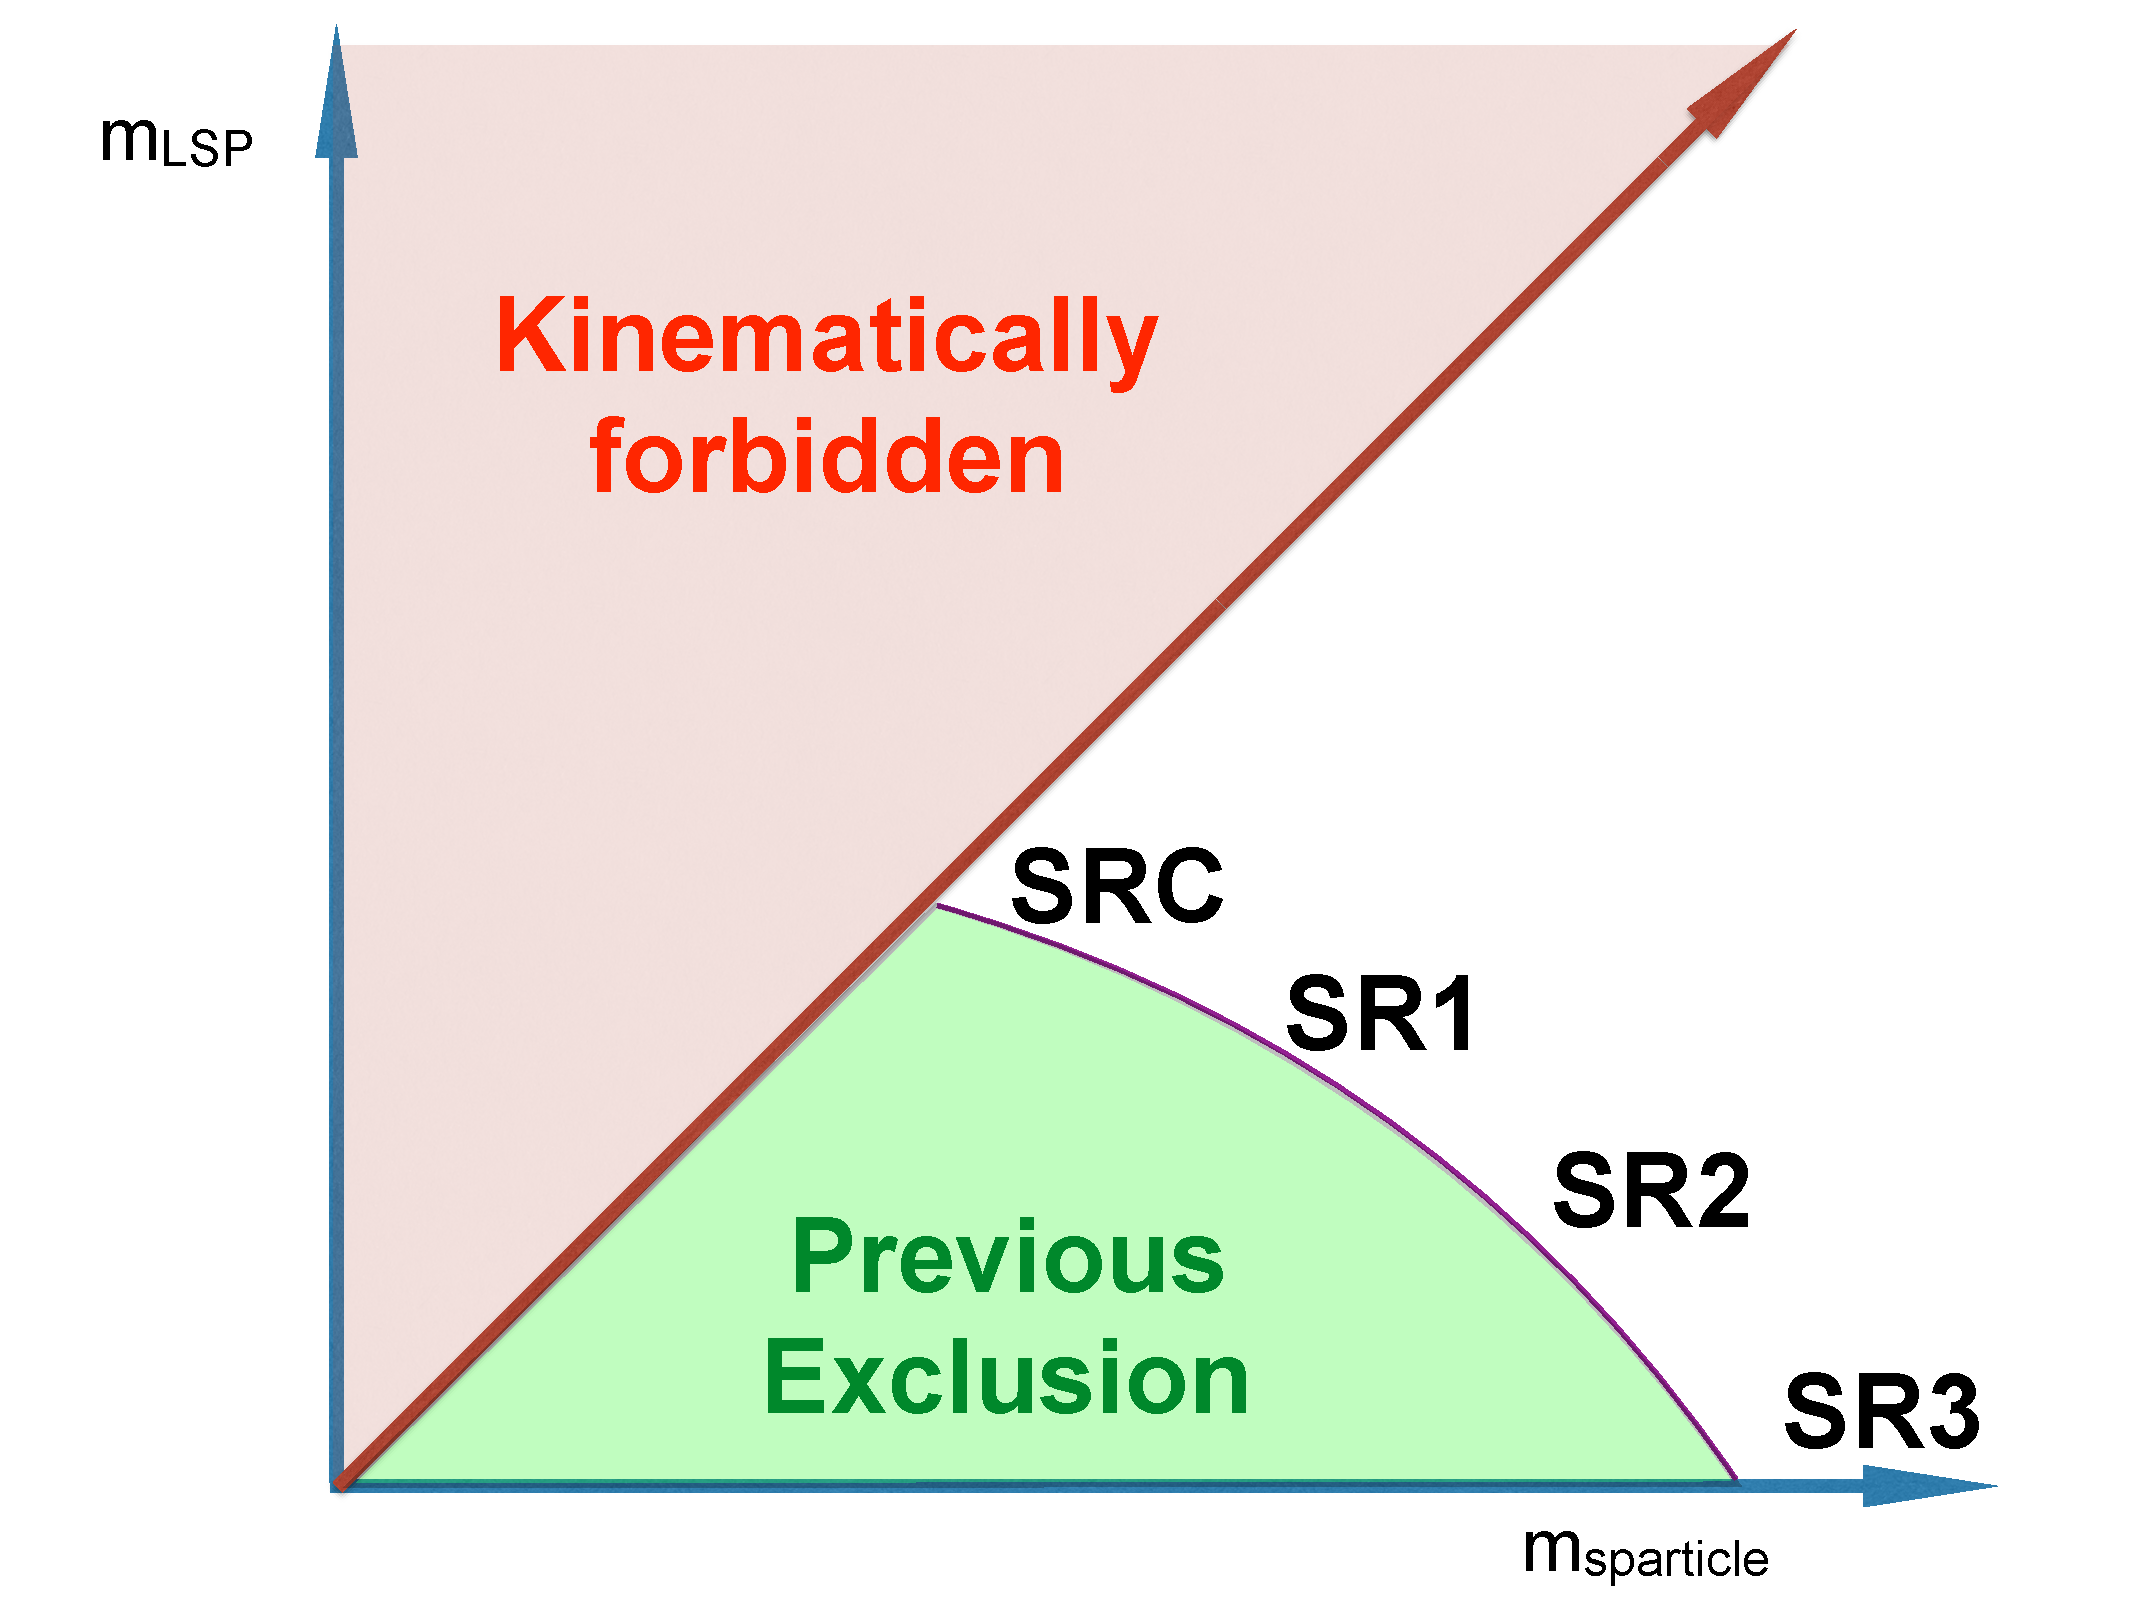
\includegraphics[width=.9\linewidth]{sr_schematic}
\end{figure}

A schematic of the signal region strategy is shown in \Cref{fig:sr_schematic}.
This type of plane is how most $R-$parity conserving SUSY searches are organized in both ATLAS and CMS.
The horizontal axis is the mass of the sparticle considered.
In the case of this thesis, this will the squark or gluino mass.
On the vertical axis, we place the LSP mass.
Thus, the grid of simplified signal models populate this plane.
Our search occurs in this two-parameter space.
Each signal region targets some portion of this plane.
A new iteration of a search will use a set of signal regions which have sensitivity just beyond those of the previous exclusions.
The choice of how many signal regions to use to cover this plane is in many ways a matter of judgment, as it is important to avoid under/over-fitting to the signal models of interest.
To take the extreme examples, one signal region will obscure the different phenomena in signal events with large versus small mass splittings, leading to underfitting.
Binning as finely as possible\footnotemark~ leads to overfitting due to the fluctuations present in the signal and background events passing the signal region selections.
In this thesis, we use six squark signal regions, six gluino signal regions, and five compressed regions.
\footnotetext{This can be defined as having a signal region for each simulated signal sample.
There are \order 200 simulated signal samples produced in the plane for the squark and gluino simplified models.}

We have described the useful variables of a RJR-based hadronic search in the previous chapter.
The question is how to choose the optimal cuts for a given set of signal models, which are grouped in the mass splitting space.
A brute force scan over the cut values to maximize the significance  $Z_{\text{Bi}}$~\cite{Cousins:2008zz} is performed, using a guess of integrated luminosity with a fixed systematic uncertainty scenario, which is motivated by previous analyses \cite{0-leptonPaper,0LPaper_13TeV}.
The squark (gluino) signal regions were optimized with a fixed 10\% (20\%) systematic uncertainty.
A figure showing an example of this selection tuning procedure is shown in \Cref{fig:sr_optimization}.

The tables which show the signal region definitions are shown in \Cref{tab:squark_srs,tab:gluino_srs,tab:compressed_srs}.
In all cases, the signal region selections contain a combination of scaleful and scaleless cuts.
Emphasis on cuts on scaleful variables provides stronger sensitivity to larger mass splittings, while additional sensitivity to smaller mass splittings is found using stronger cuts on scaleless variables.
One envisions walking from SR1 (with tight scaleless cuts and loose scaleful cuts) in \Cref{fig:sr_schematic} towards SR3 by loosening the scaleless cuts and tightening the scaleful cuts.
We will see this strategy at work in each set of signal regions.

\begin{figure}[tbp]
\caption{Optimization of the \HTFnm{PP}{4}{1} cut for a gluino signal model with $(m_{\gluino}, m_{\lsp} ) = (1500,700) \GeV $ assuming 10 \ifb~ and an uncertainty of 20\% on the background estimate.
} \label{fig:sr_optimization}
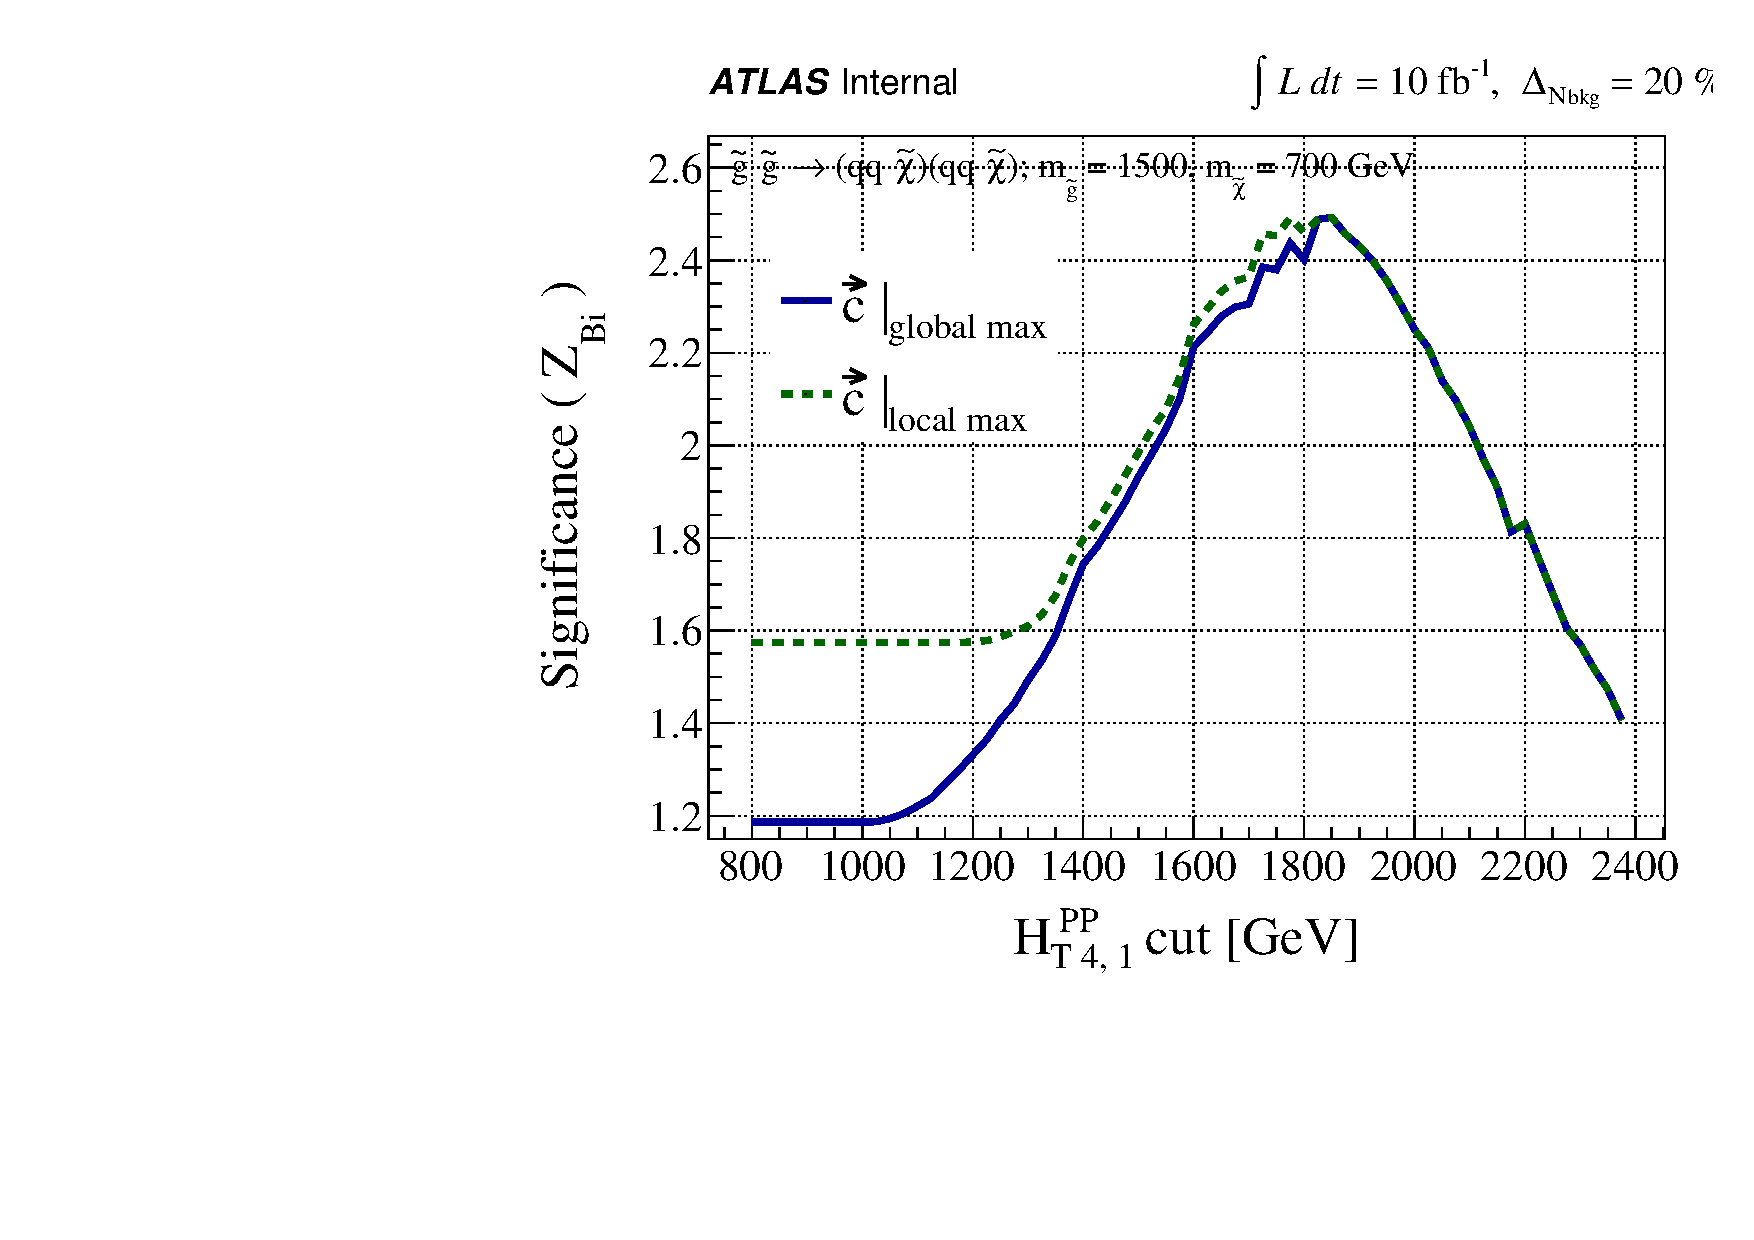
\includegraphics[width=.9\linewidth]{ATLAS-CONF-2016-078_INT/OPT_gluino/HT5PP_10fb_20sys_gg1500_700}
\end{figure}

The compressed selections are split into five regions (SRC1-5), and due to the simplified nature of the compressed decay tree, has sensitivity in both the gluino and squark planes.
The compressed regions target mass splittings with $m_{\text{sparticle}} - m_{\text{LSP}} \tilde{<} 200 \GeV$.
For the compressed region, $M_{T, S}$, our estimator for the total invariant mass of the disparticle system, is the primary scaleful variable.
The general strategy of tightening scale cuts while loosening scaleless cuts can be seen with this set of signal regions.
SRC1 targets the most compressed scenarios, with mass splittings of less than 25 \GeV, and it has the loosest $M_{T, S}$ cut.
In contrast, it has the tightest cuts on \risr, the ratio of the LSP mass to the sparticle mass, and \dphiISR, the opening angle between the invisible system and the ISR system, of the compressed signal regions..
SRC4 and SRC5 target mass splittings of $\order 200 \GeV$, and are coupled with the loosest scaleless cuts on \risr and \dphiISR.
We also note that SRC4 and SRC5 have differing cuts on \NVjet, the number of jets which are \textit{not} associated to the ISR system, since these SRs are closest in phase space to the noncompressed regions.
This can be see as the ``crossover'' in the sparticle-LSP plane where the differences between squark and gluino production begin to become manifest.

The squark regions (for noncompressed spectra) are organized into six signal regions.
These are labeled by a numeral 1-3 and letter a/b.
SRs sharing a common numeral i.e. SRS1a and SRS1b share a common set of scaleless cuts, while differing in the main scale variable \HTFnm{PP}{2}{1}.
The two SRs for each set of scaleless cuts, only differing in the main scale variable, can be seen as providing sensitivity to a range of luminosity scenarios\footnotemark.
\footnotetext{These SRs were defined before the entire collision dataset was produced, and thus needed to be robust to a range of delivered integrated luminosity.}
The scaleless cuts are loosened as we tighten the scaleful cuts, moving across the table from SRS1a to SRS3b.
This provides strong sensitivity to signal models with intermediate mass splittings with SRS1a to large mass splittings with SR3b.

The gluino signal regions are organized entirely analogously to the squark signal regions.
There are six gluino signal regions, again labeled via a numeral 1-3 and letter a/b.
Those SRs sharing a common numeral have a common set of scaleless cuts, but differ in their main scale variable \HTFnm{PP}{4}{1}.
The SRs follow the scaleless vs scaleful strategy, with SRG1 having the loosest scaleful cuts coupled with the strongest scaleless cuts, and the converse being true in SRG3.
As in the squark case, this strategy provides strong expected sensitivity throughout the gluino-LSP plane.

{
\begin{table}[tbp]
\centering
\begin{tabular}{|c|c|c|c|c|c|c|}
\hline
Targeted signal                                                                                                          & \multicolumn{6}{c|}{$\squark\squark$, $\squark \rightarrow q \lsp$}                                                                                              \\
\hline\hline
\multirow{2}{*}{Requirement}                                                                                             & \multicolumn{6}{c|}{Signal Region}                                                                                                                               \\
\cline{2-7}                                                                                                              & \multicolumn{2} {c|}{ \textbf{ S1}} & \multicolumn{2} {c|}{\textbf{S2}} & \multicolumn{2} {c|}{\textbf{S3}}                                        \\
\hline
$H_{\textrm 1,1}^{\textrm ~PP}/H_{\textrm 2,1}^{\textrm ~PP} \geq$                                                       & \multicolumn{2} {c|}{$ 0.6$}            & \multicolumn{2} {c|}{$ 0.55$}          & \multicolumn{2} {c|}{$ 0.5$}                                                  \\ \hline
$H_{\textrm 1,1}^{\textrm ~PP}/H_{\textrm 2,1}^{\textrm ~PP} \leq$                                                       & \multicolumn{2} {c|}{$ 0.95$}           & \multicolumn{2} {c|}{$ 0.96$}          & \multicolumn{2} {c|}{$ 0.98$}                                                 \\ \hline
$p_{\textrm PP,~z}^{\textrm ~lab} / \left( p_{\textrm PP,~z}^{\textrm ~lab}+H_{\textrm T~2,1}^{\textrm ~PP}\right) \leq$ & \multicolumn{2} {c|}{$ 0.5$}            & \multicolumn{2} {c|}{$ 0.55$}          & \multicolumn{2} {c|}{$ 0.6$}                                                  \\ \hline
$p_{\textrm j2,~T}^{\textrm ~PP}/H_{\textrm T~2,1}^{\textrm ~PP} \geq $                                                  & \multicolumn{2} {c|}{$ 0.16$}           & \multicolumn{2} {c|}{$ 0.15$}          & \multicolumn{2} {c|}{$ 0.13$}                                                 \\ \hline
$\Delta_{\textrm  QCD} > $                                                                                               & \multicolumn{6} {c|}{$ 0.001$}                                                                                                                                   \\
\hline\hline
                                                                                                                         & \textbf{S1a}                       & \textbf{ S1b}                      & \textbf{ S2a} & \textbf{ S2b} & \textbf{ S3a} & \textbf{ S3b} \\
\hline
$H_{\textrm T~2,1}^{\textrm ~PP}$ [GeV] $>$                                                                              & 1000                                    & 1200                                   & 1400              & 1600              & 1800              & 2000              \\
\hline
$H_{\textrm 1,1}^{\textrm ~PP}$ [GeV] $>$                                                                                & \multicolumn{2} {c|}{ 1000}             & \multicolumn{2} {c|}{ 1400}            & \multicolumn{2} {c|}{ 1600}                                                   \\
\hline
\end{tabular}
\caption{Event selection for squark signal regions
\label{tab:squark_srs}}
\end{table}

\vspace*{.01\textwidth}

\begin{table}[tbp]
\begin{tabular}{|c|c|c|c|c|c|c|}
\hline
Targeted signal & \multicolumn{6}{c|}{ $\gluino\gluino$, $\gluino \rightarrow q\bar{q} \lsp$} \\
\hline \hline
\multirow{2}{*}{Requirement}                                                                                             & \multicolumn{6}{c|}{Signal Region}                                                                                                                              \\
\cline{2-7}                                                                                                              & \multicolumn{2} {c|}{\textbf{ G1}} & \multicolumn{2} {c|}{\textbf{ G2}} & \multicolumn{2} {c|}{\textbf{ G3}}                                        \\
\hline
$H_{\textrm 1,1}^{\textrm ~PP}/H_{\textrm 4,1}^{\textrm ~PP} \geq$                                                       & \multicolumn{2} {c|}{$ 0.35$}          & \multicolumn{2} {c|}{$ 0.25$}          & \multicolumn{2} {c|}{$ 0.2$}                                                  \\ \hline
$H_{\textrm T~4,1}^{\textrm ~PP}/H_{\textrm 4,1}^{\textrm ~PP} \geq$                                                     & \multicolumn{2} {c|}{$ 0.8$}           & \multicolumn{2} {c|}{$ 0.75$}          & \multicolumn{2} {c|}{$ 0.65$}                                                 \\ \hline
$p_{\textrm PP,~z}^{\textrm ~lab} / \left( p_{\textrm PP,~z}^{\textrm ~lab}+H_{\textrm T~4,1}^{\textrm ~PP}\right) \leq$ & \multicolumn{2} {c|}{$ 0.5$}           & \multicolumn{2} {c|}{$ 0.55$}          & \multicolumn{2} {c|}{$ 0.6$}                                                  \\ \hline
min~$\left( p_{\textrm j2~T~i}^{\textrm ~PP}/H_{\textrm T~2,1~i}^{\textrm ~PP} \right) \geq$                             & \multicolumn{2} {c|}{$ 0.12$}          & \multicolumn{2} {c|}{$ 0.1$}           & \multicolumn{2} {c|}{$ 0.08$}                                                 \\ \hline
max~$\left( H_{\textrm 1,~0}^{\textrm ~Pi}/H_{\textrm 2,~0}^{\textrm Pi} \right) \leq$                                   & \multicolumn{2} {c|}{$ 0.95$}          & \multicolumn{2} {c|}{$ 0.97$}          & \multicolumn{2} {c|}{$ 0.98$}                                                 \\
\hline
$|\frac{2}{3}\Delta\phi_{\textrm V,P}^{\textrm PP} - \frac{1}{3}\cos\theta_{\textrm p} | \leq$                           & \multicolumn{2} {c|}{$ 0.5$}           & \multicolumn{4} {c|}{--}                                                                                               \\ \hline
$\Delta_{\textrm  QCD} > $                                                                                               & \multicolumn{6} {c|}{$ 0 $}                                                                                                                                     \\
\hline \hline
                                            & \textbf{ G1a}             & \textbf{ G1b}             & \textbf{ G2a}             & \textbf{ G2b} & \textbf{ G3a} & \textbf{ G3b} \\
\hline
$H_{\textrm T~4,1}^{\textrm ~PP}$ [GeV] $>$ & 1000                      & 1200                      & 1500                      & 1900 & 2300 & 2800 \\ \hline
$H_{\textrm 1,1}^{\textrm ~PP}$ [GeV] $>$   & \multicolumn{2} {c|}{600}                             & \multicolumn{2} {c|}{800}        & \multicolumn{2} {c|}{900}                   \\ \hline
\end{tabular}
\caption{Event selection for gluino signal regions
\label{tab:gluino_srs}}
\end{table}

\vspace*{.01\textwidth}

\begin{table}[tbp]
\begin{tabular}{|c|c|c|c|c|c|}
\hline
       Targeted signal & \multicolumn{5}{c|}{ compressed spectra } \\
       \hline \hline
      \multirow{2}{*}{Requirement}                                             & \multicolumn{5}{c|}{Signal Region}                                                           \\
 \cline{2-6}                                                                   & \textbf{ C1} & \textbf{ C2} & \textbf{ C3} & \textbf{ C4} & \textbf{ C5} \\
\hline
$R_{\textrm ISR} \geq $                                                        & $ 0.9$           & $ 0.85$          & $ 0.8$           & $ 0.75$          & $ 0.70$          \\ \hline
$ \Delta\phi_{\textrm ISR,~I} \geq$                                            & $ 3.1$           & $ 3.07$          & $ 2.95$          & $ 2.95$          & $ 2.95$          \\ \hline
$\ourdeltaphishort(\textrm{jet}_{\textrm 1,2},\ourvecptmiss)_{\text{min}} \> $ & -                & -                & -                & 0.4              & 0.4              \\ \hline
$M_{\textrm T S}$ [GeV] $\geq$                                                 & $ 100$           & $ 100$           & $ 200$           & $ 500$           & $ 500$           \\ \hline
$p_{\textrm T S}^{\textrm ~CM}$ [GeV]  $\ge$                                   & $ 800$           & $ 800$           & $ 600$           & $ 600$           & $ 600$           \\ \hline
$N_{\textrm jet}^{\textrm ~V} \geq$                                            & $ 1$             & $ 1$             & $ 2$             & $ 2$             & $ 3$             \\
\hline

\end{tabular}
\caption{Event selection for compressed signal regions
\label{tab:compressed_srs}}
\end{table}
}

%%% Local Variables:
%%% mode: latex
%%% TeX-master: t
%%% End:


\section{Background estimation}

We describe here the method of background estimation.
In this thesis, we detail a ``cut-and-count'' analysis.
%We contrast to a ``shape fit'' analysis, where one needs to consider the details of the variable distribution shapes.
In this type of analysis, we must ensure the Standard Model background event yields are correct in the regions of phase space considered in the analysis.
In order to do this, we define a set of \textit{control regions} which are free of SUSY contamination based on the previously excluded analysis.
We define a \textit{transfer factor} (TF) for each control region, which is defined as the ratio of the expected number of events from simulation in the signal region to the expected number from simulation of events in the control region.
Multiplying the TF by the \textit{observed} number of events in the control region gives the estimate of the number of background events in the given signal region.
To be explicit, each signal region SR has a corresponding set of control regions, where each control region is targeted towards a particular background process.

More precisely, for a given signal region, we are attempting to estimate $\ntext{SR}{data}$, the number of events entering the signal region corresponding to a particular background process.
We define a corresponding control region of high purity for that particular background process.
We observe a number of events $\ntext{CR}{data,obs}$ which pass the control region selection.
Defining $\ntext{SR}{MC}$ ($\ntext{CR}{MC}$) as the number of events in simulation passing the SR (CR) event selection, our estimate of $\ntext{SR}{data}$ can be written as:
\begin{align}\label{eq:bkg_est}
\ntext{SR}{data,est} = \ntext{CR}{data,obs} \times \text{TF}_{\text{CR}} \equiv \ntext{CR}{data,obs} \times  \begin{pmatrix} \frac{ \ntext{SR}{MC} }{ \ntext{CR}{MC} } \end{pmatrix}
\end{align}
The two ingredients to our estimation of \ntext{SR}{data,obs} are the observed number of control region events \ntext{CR}{data,obs} and the transfer factor taken from simulation.

It is illuminating to rewrite \Cref{eq:bkg_est}:
\begin{align}\label{eq:bkg_est_simple}
\ntext{SR}{data,est} = \ntext{SR}{MC} \times  \begin{pmatrix} \frac{\ntext{CR}{data,obs}  }{ \ntext{CR}{MC} } \end{pmatrix} \equiv \ntext{SR}{MC} \times \mu_{CR}.
\end{align}
In this form, the correction to SM background event yield is explicit.
The ratio $\frac{\ntext{CR}{data,obs}}{ \ntext{CR}{MC} }$, which we call $\mu_{\text{CR}}$, is the scale which corrects for our ignorance of the normalization of the particular SM background.
The assumption of this method is the overall shape of the distribution should not change as one extrapolates to the signal region.

The CR definitions are motivated and designed according to two (generally competing) requirements:
\begin{enumerate}
\item Statistical uncertainties due to low numbers of events passing the control region selections
\item Systematic uncertainties on the extrapolation from the CR to the SR.  These are minimized by creating control regions which are as similar as possible to the signal regions without risking signal contamination while ensuring high purity in the targeted SM background.
\end{enumerate}
In principle, one can also apply data-driven corrections to the TF obtained for each CR.

In order to validate the transfer factors obtained from MC, we also develop a series of \textit{validation regions} (VRs).
These regions are generally designed to be ``in between'' the control region and signal region selections in phase space, and thus provide a check on the extrapolation from the control regions into the signal regions.
Despite their closeness in phase space to the signal regions, they are also designed to have low signal contamination.

We perform this estimation procedure simultaneously across all control regions.
Note \Cref{eq:bkg_est} can also be used to measure the contamination of a control region with another background, as determined by another control region.

\subsection{Maximum likelihood fit}

To properly account for the systematic uncertainties and simultaneously fit the control regions, we employ a maximum-likelihood fit as described in \cite{Baak:2014wma}.
The likelihood function \Lagr is the product of the Poisson distributions governing the likelihood in each of the signal regions and the corresponding control regions.
We begin by considering our event counts  $\bm{b}$ in a signal region with its corresponding control regions.
The systematic uncertainties are included as a set of nuisance parameters $\bm{\theta}$.

The full likelihood function can be written ~\cite{Baak:2014wma}:
\begin{align}
\Lagr(n | \mu, b) &= P_{\mathrm{SR}} \times P_{\mathrm{CR}} \times C_{\mathrm{syst}} \\
                  &= P(n_S | \lambda_S(\mu_{S},  \bm{b}, \bm{\theta} ) ) \times
                     \prod_{i \epsilon \text{CR}}  P(n_i | \lambda_i(\mu_b , \bm{b}, \bm{\theta}))
                     \times C_{\text{syst}}(\bm{\theta}^0 , \bm{\theta})
\end{align}
where $P(n_i | \lambda_i(\mu , \bm{b}, \bm{\theta}))$ is a Poisson distribution conditioned on the event counts $n_i$ in the $i$-th CR with mean parameter $\lambda_i(\mu , \bm{b}, \bm{\theta})$.
The term $C_{\text{syst}}(\bm{\theta}^0 , \bm{\theta})$ is the probability density function with central values $\bm{\theta}^0$ which are varied with the nuisance parameters $\bm{\theta}$.
We model these as Gaussian distributions with unit width and mean zero:
\begin{align}
C_{\text{syst}}(\bm{\theta}^0 , \bm{\theta}) = \prod_{s\epsilon S} G(\mu = \theta_s, \sigma = 1),
\end{align}
where $S$ is the set of systematic uncertainties.

The terms $\lambda_j$ for any region $j$ can be expressed as
\begin{align}
\lambda_j( \mu, \bm{b},\bm{\theta}) = \sum_b \mu_b \xspace b_j \xspace \prod_{s\epsilon S} \xspace (1 + \Delta_{j,b,s} \theta_s)
\end{align}
The term $\mu_b$ is the normalization factor associated to the background $b$ with event count $b_j$ in the region $j$.
The terms $\bm{\Delta}$ inside the product represent scale factors freeing the model to account for the systematic uncertainties $\theta_s$.

The process now is to maximize this likelihood function, given the free parameters $\mu_b$ and the parameters $\bm{\Delta}$ associated to the systematics as nuisance parameters.
This is done using the \histfitter~ package ~\cite{Baak:2014wma}.
The normalization scale factors $\mu_b$ are the primary output of this maximization, and are in fact the control regions' raison d'\^{e}tre.
%We maximize the likelihood function su magnitudes of each background process \textit{given the actual control region event counts}.
We say the normalization parameters are found such that the likelihood is maximized.
The nuisance parameters are also determined by this procedure, but do not have a straightforward interpretation.

The final expected background prediction after the fit in region $r$ is given by
\begin{align}
N_{r,\text{total background}} = \sum_b \mu_b N_{b, \text{MC}}
\end{align}
We next describe the control regions used in the analysis.

\subsection{Control Regions}

The primary backgrounds in this analysis are \zjets, \wjets, \ttbar, and QCD events.
There is also a minor background from diboson events which is taken directly from simulation with an ad-hoc uncertainty of 50\%.
We describe the strategy to estimate these various backgrounds here.
A summary table is shown in \Cref{tab:crdefs}.
All distributions shown in this section use the scaling factors $\mu$ from the background fits.
\begin{table}[tbp]
\scriptsize
\begin{center}\renewcommand\arraystretch{1.2}
%\resizebox{\textwidth}{!}{
\begin{tabular}{| l | c | c | c | c |}
\hline
CR                  & SM background                  & CR process                       & CR event selection                        \\
 \hline \hline
CR$\gamma$ & $Z(\to\nu\bar\nu)$+jets        & $\gamma$+jets                    & Isolated photon                                           \\ \hline
CRQ        & Multi-jet                      & Multi-jet                        & $\Delta_{\mathrm  QCD} < 0$                               \\
           &                                &                                  & reversed requirement on                                   \\
           &                                &                                  & $H_{\mathrm 1,1}^{\mathrm ~PP} $ (RJR-S/G)                \\
           &                                &                                  & or $R_{\mathrm ISR} <$ 0.5 (RJR-C)                        \\ \hline
CRW        & $W(\to\ell\nu)$+jets           & $W(\to\ell\nu)$+jets             & 30~\GeV $<m_{\mathrm  T}(\ell,\met) < 100$~\GeV, $b$-veto \\ \hline
CRT        & $t\bar{t}$(+EW) and single top & $t\bar{t}\to b\bar{b}qq'\ell\nu$ & 30~\GeV $<m_{\mathrm  T}(\ell,\met) < 100$~\GeV, $b$-tag  \\
\hline
\end{tabular}
\caption{\label{tab:crdefs}
Control regions used in this thesis.
}
\end{center}
\end{table}

%%% Local Variables:
%%% mode: latex
%%% TeX-master: t
%%% End:


Events with a $Z$ boson decaying to neutrinos in association with jets are the primary irreducible background in the analysis.
These events have true \met from the decaying neutrinos, and can have large values of the RJR scaleful variables described in \Cref{sec:rjr_hadronic}.
Naively, one might expect us to use \Zll as the control process, as \Zll events are well-measured.
Unfortunately, the \Zll branching ratio is about half of from \Zvv, which necessitates loosening the control region selection significantly.
This leads to unacceptably large systematic uncertainties in the transfer factor.

Instead, photon events are used as the control region for the \Zvv events.
We label this photon control region as CR$\gamma$.
The photon is required to have $\pt > 150 \GeV$ to ensure the trigger is fully efficient.
The kinematic properties of photon events strongly resemble those of $Z$ events when the boson \pt is significantly above the mass of the $Z$ boson.
In this regime, the neutral bosons are both scaleless, and can be treated interchangeably, up to the differences in coupling strengths.
%There are some residual effects due to the differing spin states, which should be identifiable in events with
Additionally, the cross-section for \gammajets~ events is significantly larger than \zjets~ events above the $Z$ mass.
These features are shown in \Cref{fig:boson_pt_ratio} in simulated \Zvv truth events.
In truth events, one clearly sees the effect of the $Z$ mass below \order 100 \GeV, with a flattening of the ratio above \order 300 \GeV.

The CR$\gamma$ kinematic selection is slightly looser in the scaleful variables for the noncompressed regions for sufficient control region statistics.
This is chosen to be $\HFnm{PP}{1}{1} > 900 \GeV$ ($\HFnm{PP}{1}{1} > 550 \GeV$) for the squark (gluino) regions to minimize the corresponding statistical and systematic uncertainties.
\begin{figure}[tbp]
\caption{Boson \pt ratio as a function of true boson \pt} \label{fig:boson_pt_ratio}
\includegraphics[width=.9\linewidth]{ATLAS-CONF-2016-078_INT/GammaReweighting/Znunu_truth_bosonPt_dPhi/c1_bosonPt_no_cuts}
%\subfloat[Boson \pt ratio as a function of reconstructed boson \pt]{\includegraphics[width=.45\linewidth]{ATLAS-CONF-2016-078_INT/GammaReweighting/Znunu_reco/c1_bosonPt_no_cuts}}
\end{figure}

One additional correction scale factor is applied to \gammajets~ events before calculating the transfer factors.
This is known as the $\kappa$ method, which is used to determine the disagreement arising from the use of a LO generator for photon events vs. a NLO generator for \zjets~ events, which can reduce the theoretical uncertainties.
One can see this as a measurement of the k-factor for the LO \gammajets~ sample.
% We employ an auxiliary CRZ region, defined using two leptons with an invariant mass within 25 \GeV of the $Z$ mass.
% Adding the \pt of the two leptons into the \met, we require $200 \GeV < \met < 300 \GeV$.
% Defining an equivalent CR$\gamma$ region, with the photon \pt included in the \met calculation, and requiring $200 \GeV < \met < 300 \GeV$
We define two \textit{very loose} control regions, CRZVL and CR$\gamma$VL.
CRZVL requires two leptons with an invariant mass within 25 \GeV of the $Z$ mass.
We add the \pt of the leptons into the \met, as done in CR$\gamma$, and require $200 \GeV < \met < 300 \GeV$.
CR$\gamma$VL uses the same \met requirement, with the photon included in the \met calculation.
With the data event counts in these regions $N_{CR\gamma VL}^{\gamma\mathrm{+jets,data}}$ and $N_{CRZVL}^{\Zll\mathrm{+jets,data}}$ and the predictions from simulation $N_{CR\gamma VL}^{\gamma\mathrm{+jets,MC}}$ and $N_{CRZVL}^{\Zll\mathrm{+jets,MC}}$, we define
\begin{align}
\kappa \equiv \Big( \frac{N_{CR\gamma VL}^{\gamma\mathrm{+jets,data}}}{N_{CRZVL}^{\Zll\mathrm{+jets,data}}} \Big) \Big/ \Big( \frac{N_{CR\gamma VL}^{\gamma\mathrm{+jets,MC}}}{N_{CRZVL}^{\Zll\mathrm{+jets,MC}}} \Big)
\end{align}
Additional details can be found in ~\cite{0-leptonPaper,0LPaper_13TeV,ATLAS-CONF-2016-078}.
The correction factor is $\kappa = 1.39 \pm 0.05$.
The uncertainty is derived from the calculation of $\kappa$ with the \met requirements for CRZVL and CR$\gamma$VL changed.

Distributions of CR$\gamma$ in squark, gluino, and compressed regions are shown in \Cref{fig:CRY_SRJigsawSRG1a_LastCut_CRY_minusone,fig:CRY_SRJigsawSRC1_LastCut_CRY_minusone}.
These figures show the high purity of the photon control region for each signal region.

Event with a $W$ boson decaying leptonically via \wln can also enter the signal region.
%In this case, we  include all leptons ($e,\mu,\tau$).
The \wjets~ events passing the event selection either have a hadronically-decaying $\tau$, with a neutrino supplying \met, or a muon or electron is misidentified as a jet or missed completely due to the limited detector acceptance.
To model the \wjets~ background, we use a sample of one-lepton events with a veto on b-jets, which we label CRW.
The lepton is required to have $\pt > 27 \GeV$ to guarantee a fully efficient trigger.
We treat this single lepton as a jet for purposes of the RJR variable calculations.
We apply a kinematic selection on the transverse mass:
\begin{align}
m_T = \sqrt{2p_{T,\ell} \met ( 1 - \cos{ \phi_{e} - \metphi } ) },
\end{align}
around the $W$ mass: $30 \GeV < m_T < 100 \GeV$.
Checks in simulation shows that these requirements give a sample of high purity \wln background.
Due to low statistics using the kinematic cuts imposed in the signal regions, the control region kinematic cuts are slightly loosened with respect to the signal region cuts.
They are loosened in a way that inside each class of signal regions (SRS, SRG, SRC) the same CRW is used.
We use the loosest cut for each variable among \textit{any} signal region in the selection of CRW.
For example, the control region CRW for SRS1a uses the following kinematic selections after the one lepton, $b$-veto selection is imposed:
\begin{table}[H]
\label{tab:crw_kinematic_selection}
\begin{tabular}{|l|l|}
\hline
Variable & CRW cut \\ \hline
$H_{\textrm 1,1}^{\textrm ~PP}/H_{\textrm 2,1}^{\textrm ~PP} \geq$ & 0.5 \\ \hline
$H_{\textrm 1,1}^{\textrm ~PP}/H_{\textrm 2,1}^{\textrm ~PP} \leq$ & 0.98 \\ \hline
$p_{\textrm PP,~z}^{\textrm ~lab} / \left( p_{\textrm PP,~z}^{\textrm ~lab}+H_{\textrm T~2,1}^{\textrm ~PP}\right) \leq $ & 0.6 \\ \hline
$p_{\textrm j2,~T}^{\textrm ~PP}/H_{\textrm T~2,1}^{\textrm ~PP} \geq $ & 0.13 \\ \hline
$\Delta_{\textrm  QCD} > $ & 0.001 \\ \hline
$H_{\textrm T~2,1}^{\textrm ~PP}>$ & 1000 \GeV \\ \hline
$H_{\textrm 1,1}^{\textrm ~PP} >$ & 1000 \GeV \\ \hline
\hline
\end{tabular}
\end{table}
Comparing this set of selections with the signal regions \Cref{tab:squark_srs}, these are loosest cuts among all squark signal regions.
This leads to a tolerable increase in the systematic uncertainty from the extrapolation from the CR to the SR when compared to the resulting statistical uncertainty.

Distributions of CRW in squark, gluino, and compressed regions are shown in \Cref{fig:CRW_SRJigsawSRG1a_LastCut_CRW_minusone,fig:CRW_SRJigsawSRC1_LastCut_CRW_minusone}.
There is high purity in \wjets~events in the control region corresponding to all signal regions.

Top events are also an important background, for the same reasons as the \wjets~ background, due to the dominant top decay channel of $t \rightarrow Wb$.
For a top event to be selected by the analysis criteria, we expect a similar process to that of the \wjets background.
The $W$ decays via a $\tau$ lepton which decays hadronically or the $W$ decays via a muon or electron which is misidentified as a jet or falls outside the detector acceptance.
Hadronic or all dileptonic tops are less troublesome, as hadronic \ttbar events generally have low \met (and \HFnm{PP}{1}{1}) and will not pass the kinematic selections, while dileptonic \ttbar events have a lower cross-section and good reconstruction efficiency from the two leptons.
We are thus primarily concerned with semileptonic \ttbar events with \met from the neutrino.
To model this background, we use the same selection as the $W$ selection, but require that one of the jets chosen by the analysis has at least one $b$-tag.
This selection has high purity, as we expect the \ttbar background to have two $b$-jets.
With the 70\% $b$-tagging efficiency working point~\cite{Aad:2015ydr,ATL-PHYS-PUB-2016-012}, ignoring (small) correlations between the two $b$-tags, we expect to tag one of the $b$-jets greater than 90\% of the time.
We use the same loosening scheme as we described for CRW.
Using the SRS1a example in \Cref{tab:crw_kinematic_selection}, we implement the same kinematic cuts applied as in CRW, but with the required $b$-jet instead of a $b$-jet veto.

Distributions of CRT in squark, gluino, and compressed regions are shown in \Cref{fig:CRT_SRJigsawSRG1a_LastCut_CRT_minusone,fig:CRT_SRJigsawSRC1_LastCut_CRT_minusone}.
There is high purity in top events in the control region corresponding to all signal regions.

QCD events are another important background.
QCD backgrounds are difficult, for a few reasons.
The large cross-section for QCD events means that even very rare extreme mismeasurements can be seen in our signal regions.
However, as these events are very rare, simulation fails to be a particularly useful input for background estimation, as the details of these extraordinary events are poorly modeled.
Instead, we apply a cut which ensures \textit{zero} QCD events in the signal regions.
To produce a sample enriched in QCD, which we call CRQ, we invert the $\Delta_{\mathrm{QCD}}$ and \HFnm{PP}{1}{1} cut from the corresponding signal region.
This means instead of requiring these values over the signal region cut, we require them to be under the signal region cut.
This analysis uses the jet smearing method, as described in ~\cite{SUSY-2011-20}.
%This is a data-driven method which applies a resolution function to well-measured QCD events, which also an estimate of the impact of the jet energy mismeasurement on \met and subsequently the RJR variables.

Distributions of CRQ in squark, gluino, and compressed regions are shown in \Cref{fig:CRQ_SRJigsawSRG1a_LastCut_CRQ_minusone,fig:CRQ_SRJigsawSRC1_LastCut_CRQ_minusone}.
There is high purity in QCD events in the control region corresponding to all signal regions.

Diboson events can also pass the signal region selection criteria.
This background is estimated directly from simulation.
Due to the low cross-section of electroweak processes, this background is not significant in the signal regions.
We assign a large ad-hoc 50\% systematic on the cross-section, and do not attempt to define a control region for this background.

\begin{figure}[tbph]
\begin{center}
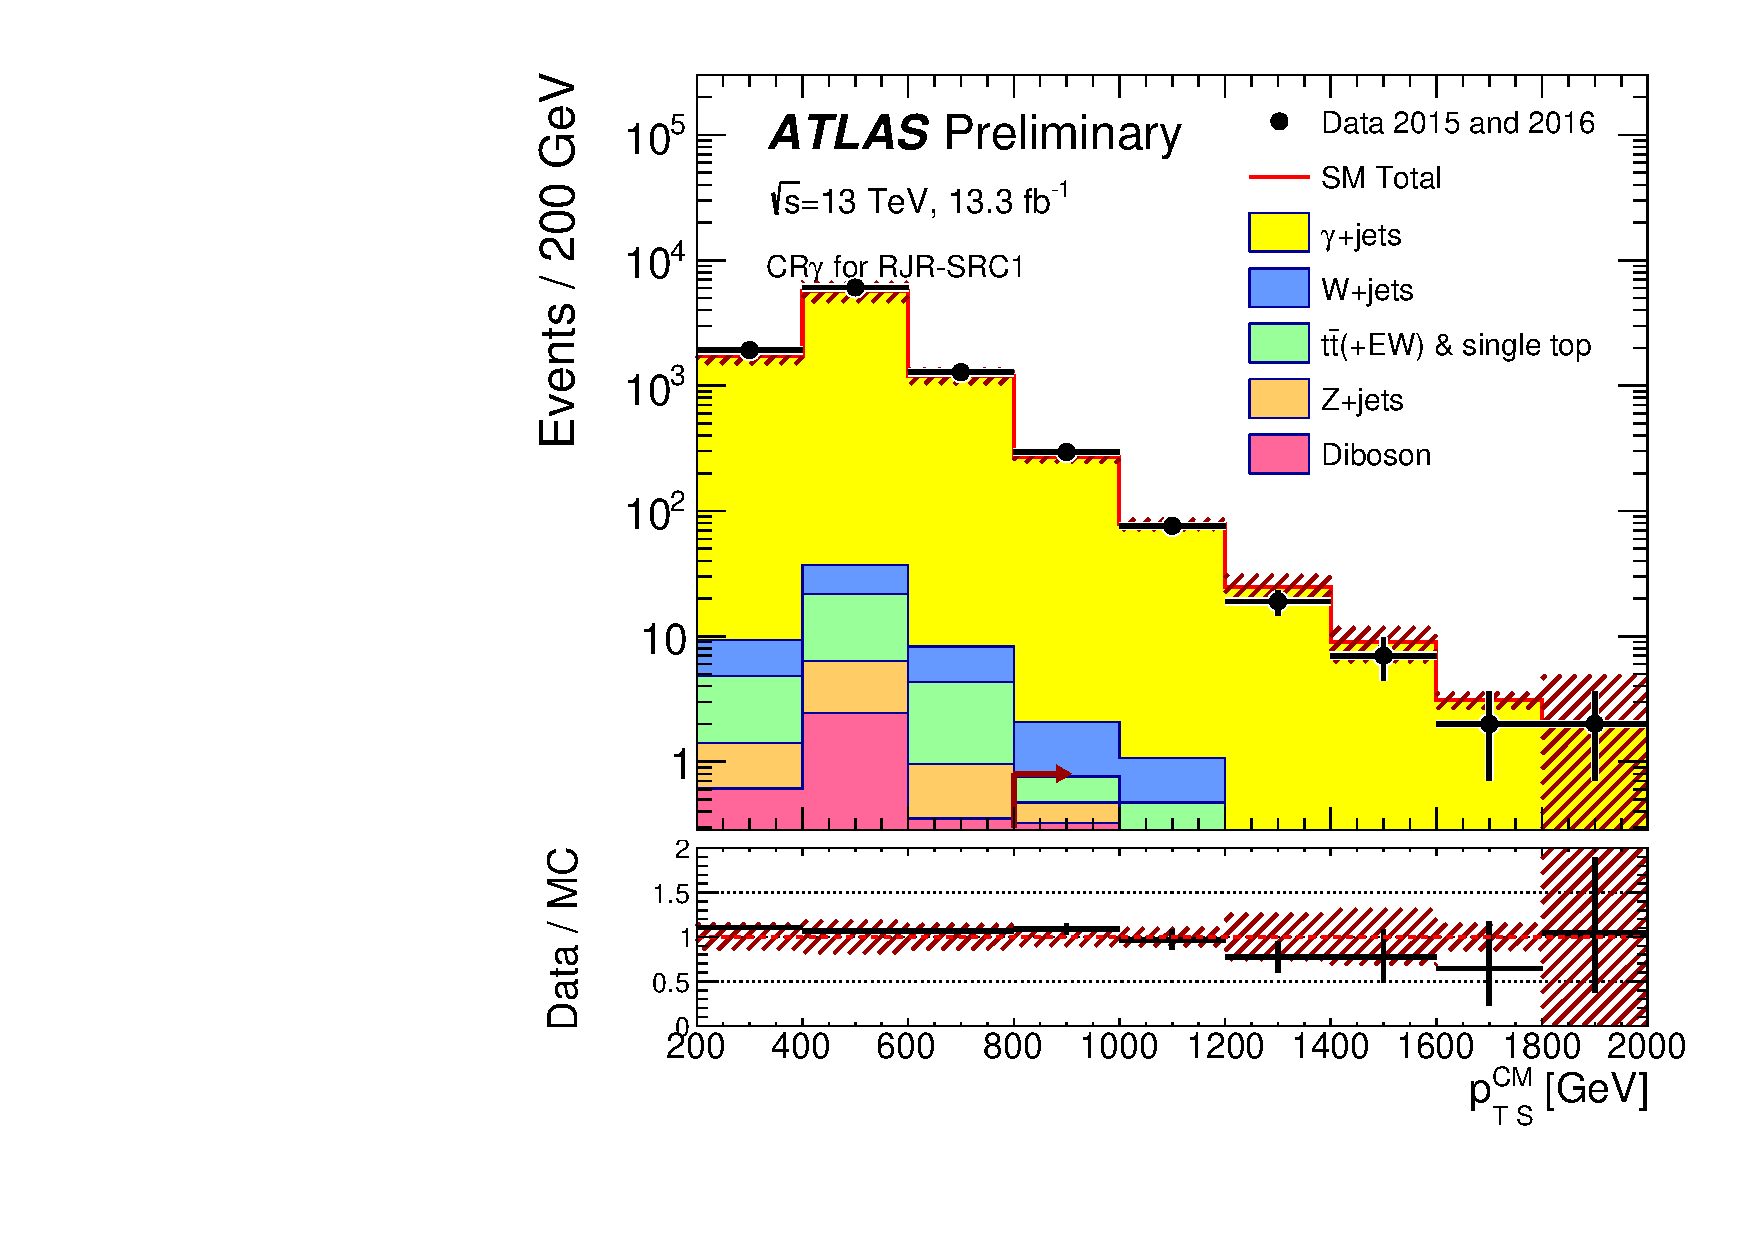
\includegraphics[width=0.45\textwidth]{figures/ATLAS-CONF-2016-078_INT/N-1Plots/AtlasStyle/Preliminary/CRY_SRJigsawSRC1_LastCut_CRY_minusone}
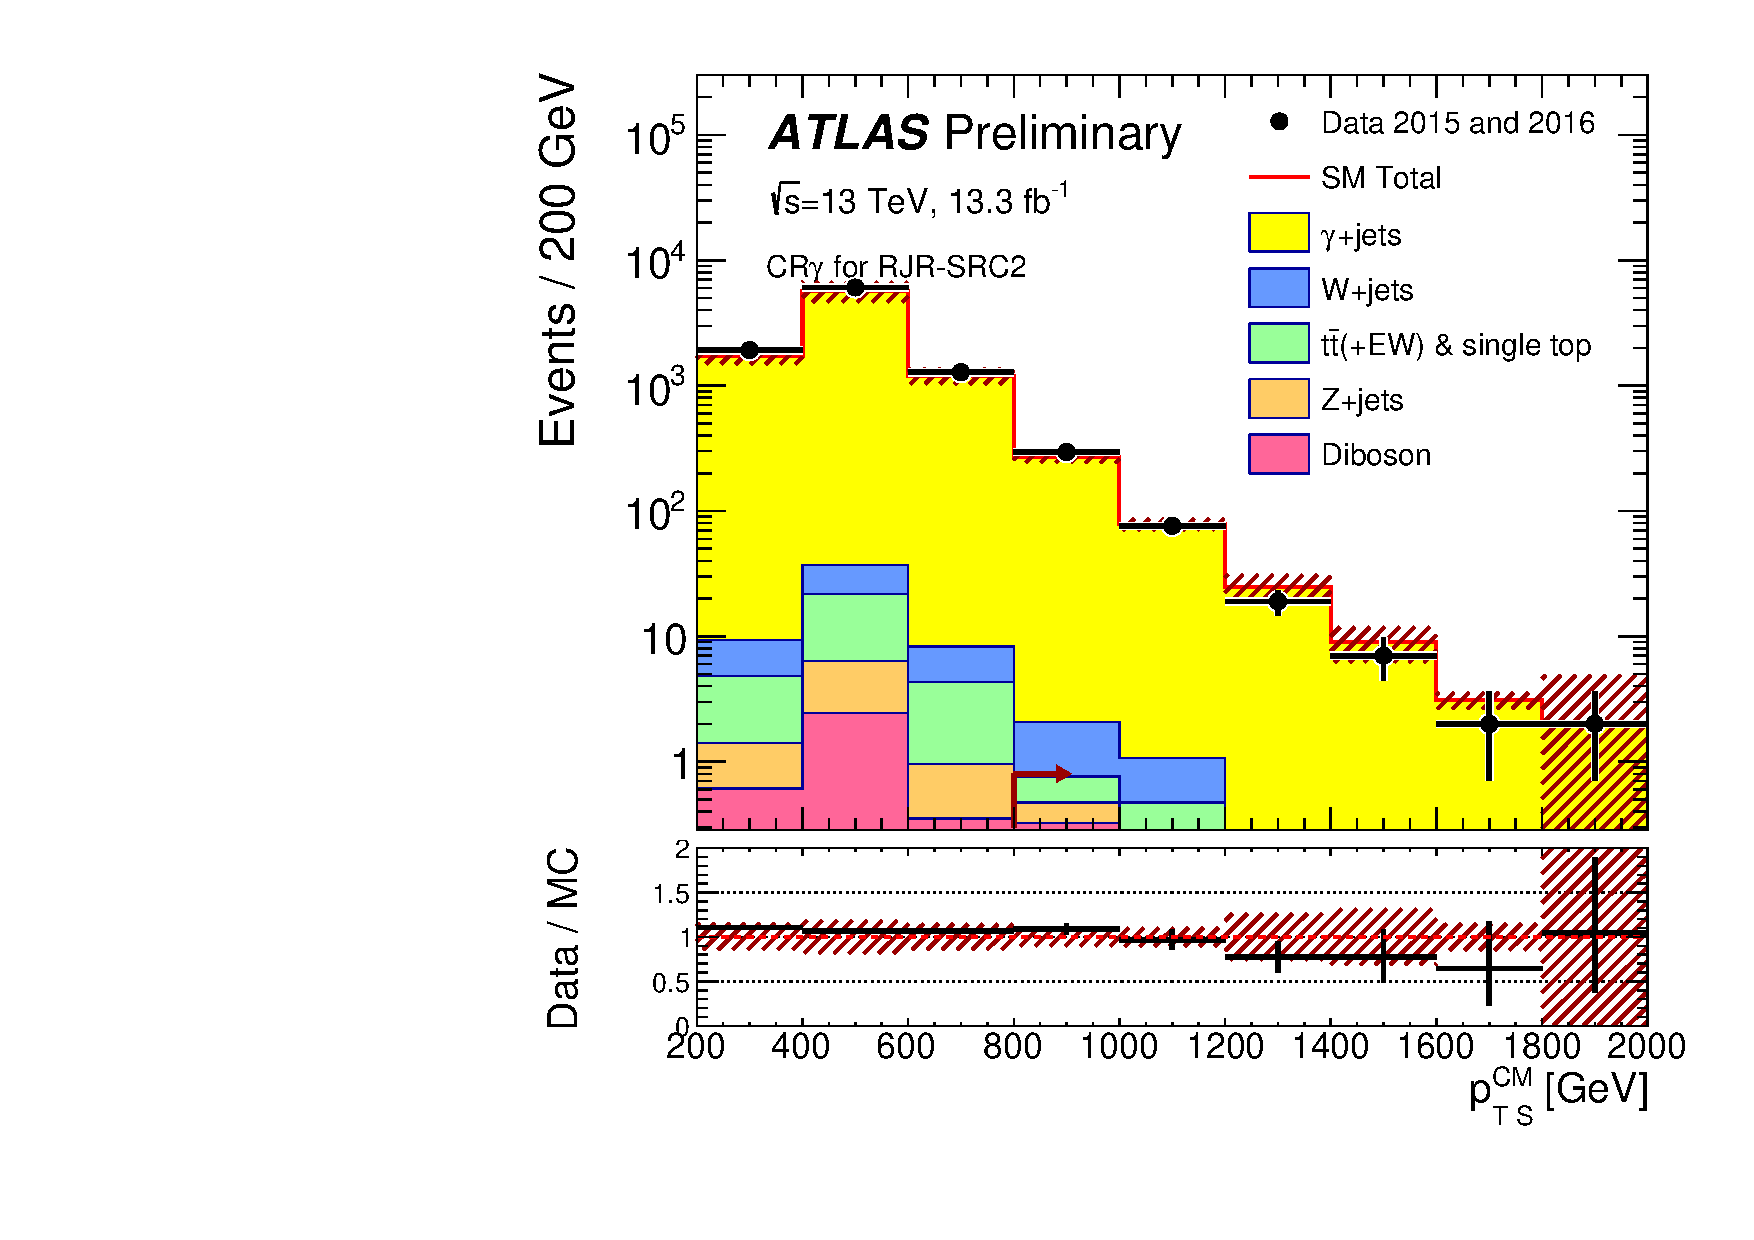
\includegraphics[width=0.45\textwidth]{figures/ATLAS-CONF-2016-078_INT/N-1Plots/AtlasStyle/Preliminary/CRY_SRJigsawSRC2_LastCut_CRY_minusone}
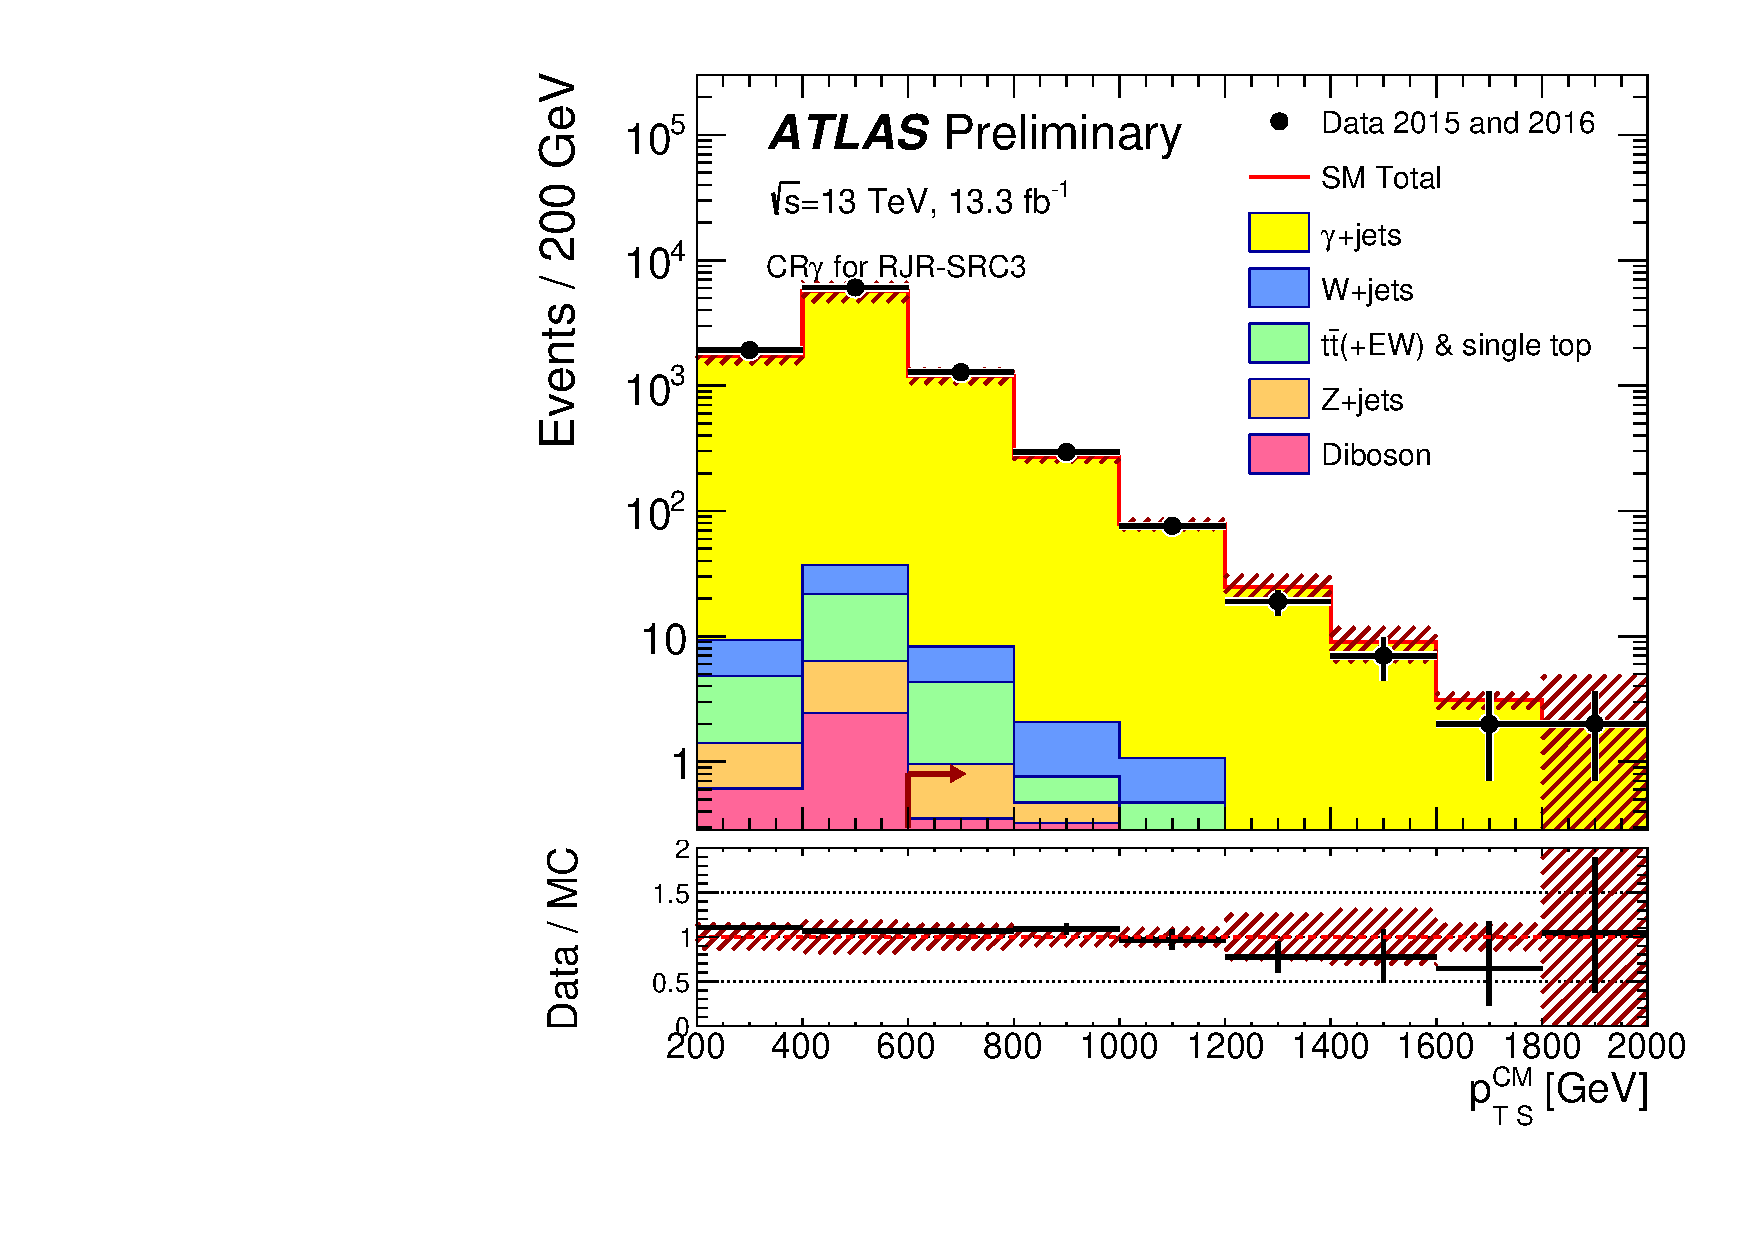
\includegraphics[width=0.45\textwidth]{figures/ATLAS-CONF-2016-078_INT/N-1Plots/AtlasStyle/Preliminary/CRY_SRJigsawSRC3_LastCut_CRY_minusone}
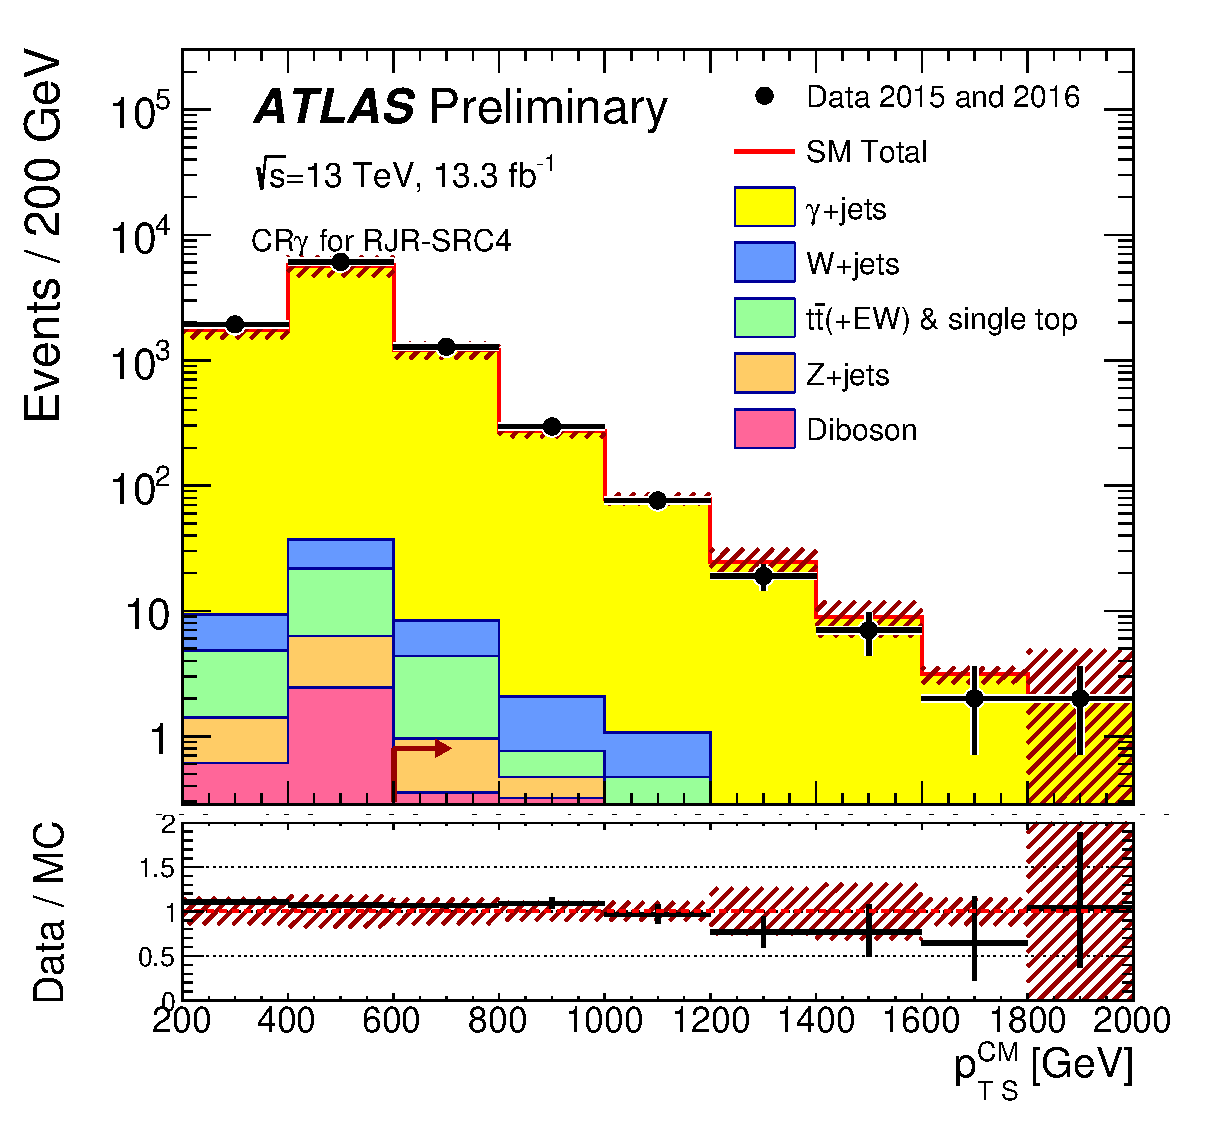
\includegraphics[width=0.45\textwidth]{figures/ATLAS-CONF-2016-078_INT/N-1Plots/AtlasStyle/Preliminary/CRY_SRJigsawSRC4_LastCut_CRY_minusone}
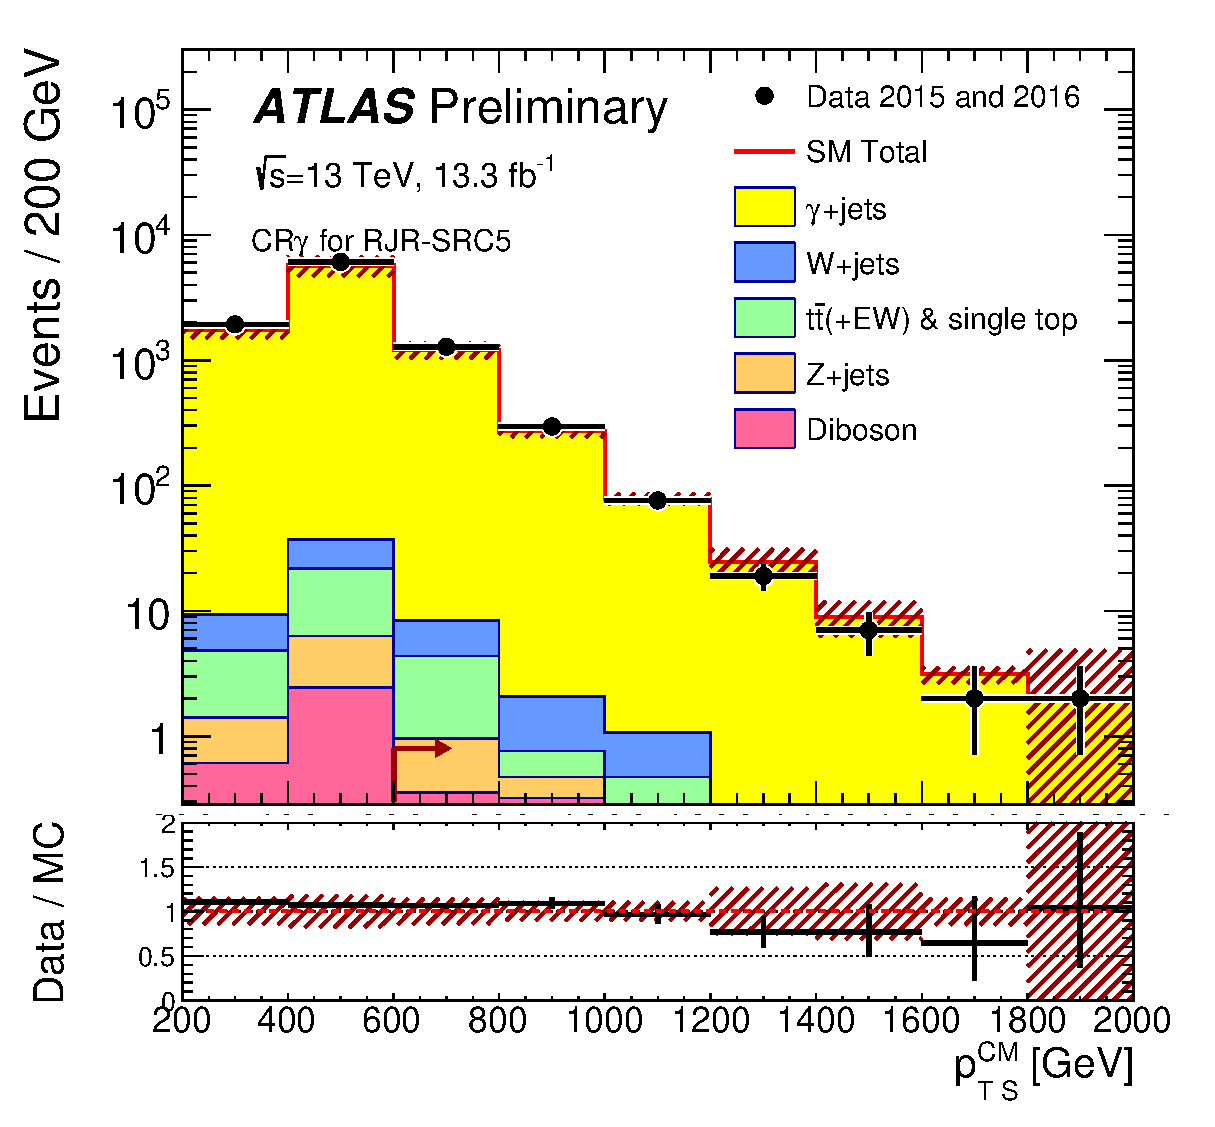
\includegraphics[width=0.45\textwidth]{figures/ATLAS-CONF-2016-078_INT/N-1Plots/AtlasStyle/Preliminary/CRY_SRJigsawSRC5_LastCut_CRY_minusone}
\end{center}
\caption{Scale variable distributions for the compressed CRY regions.}
\label{fig:CRY_SRJigsawSRC1_LastCut_CRY_minusone}
\end{figure}

\begin{figure}[tbph]
\begin{center}
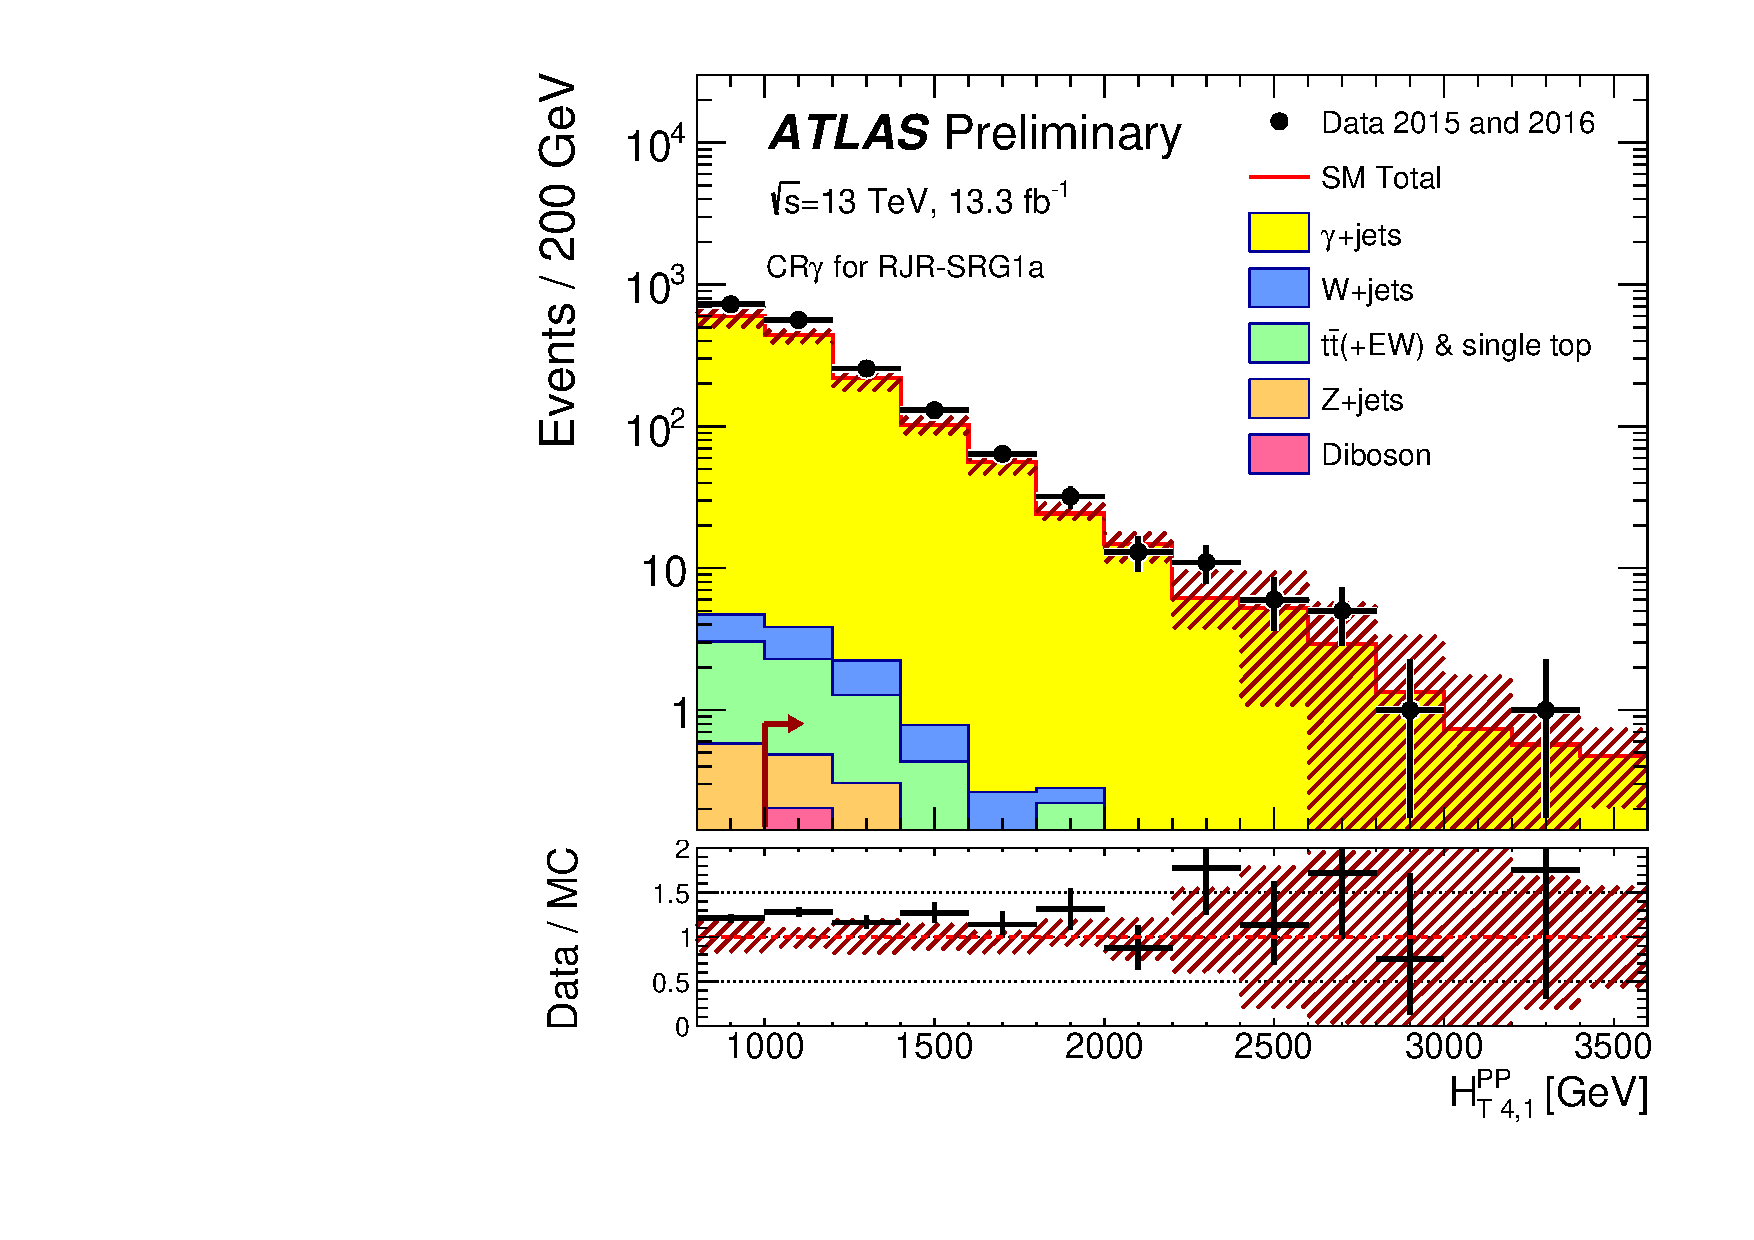
\includegraphics[width=0.45\textwidth]{figures/ATLAS-CONF-2016-078_INT/N-1Plots/AtlasStyle/Preliminary/CRY_SRJigsawSRG1a_LastCut_CRY_minusone}
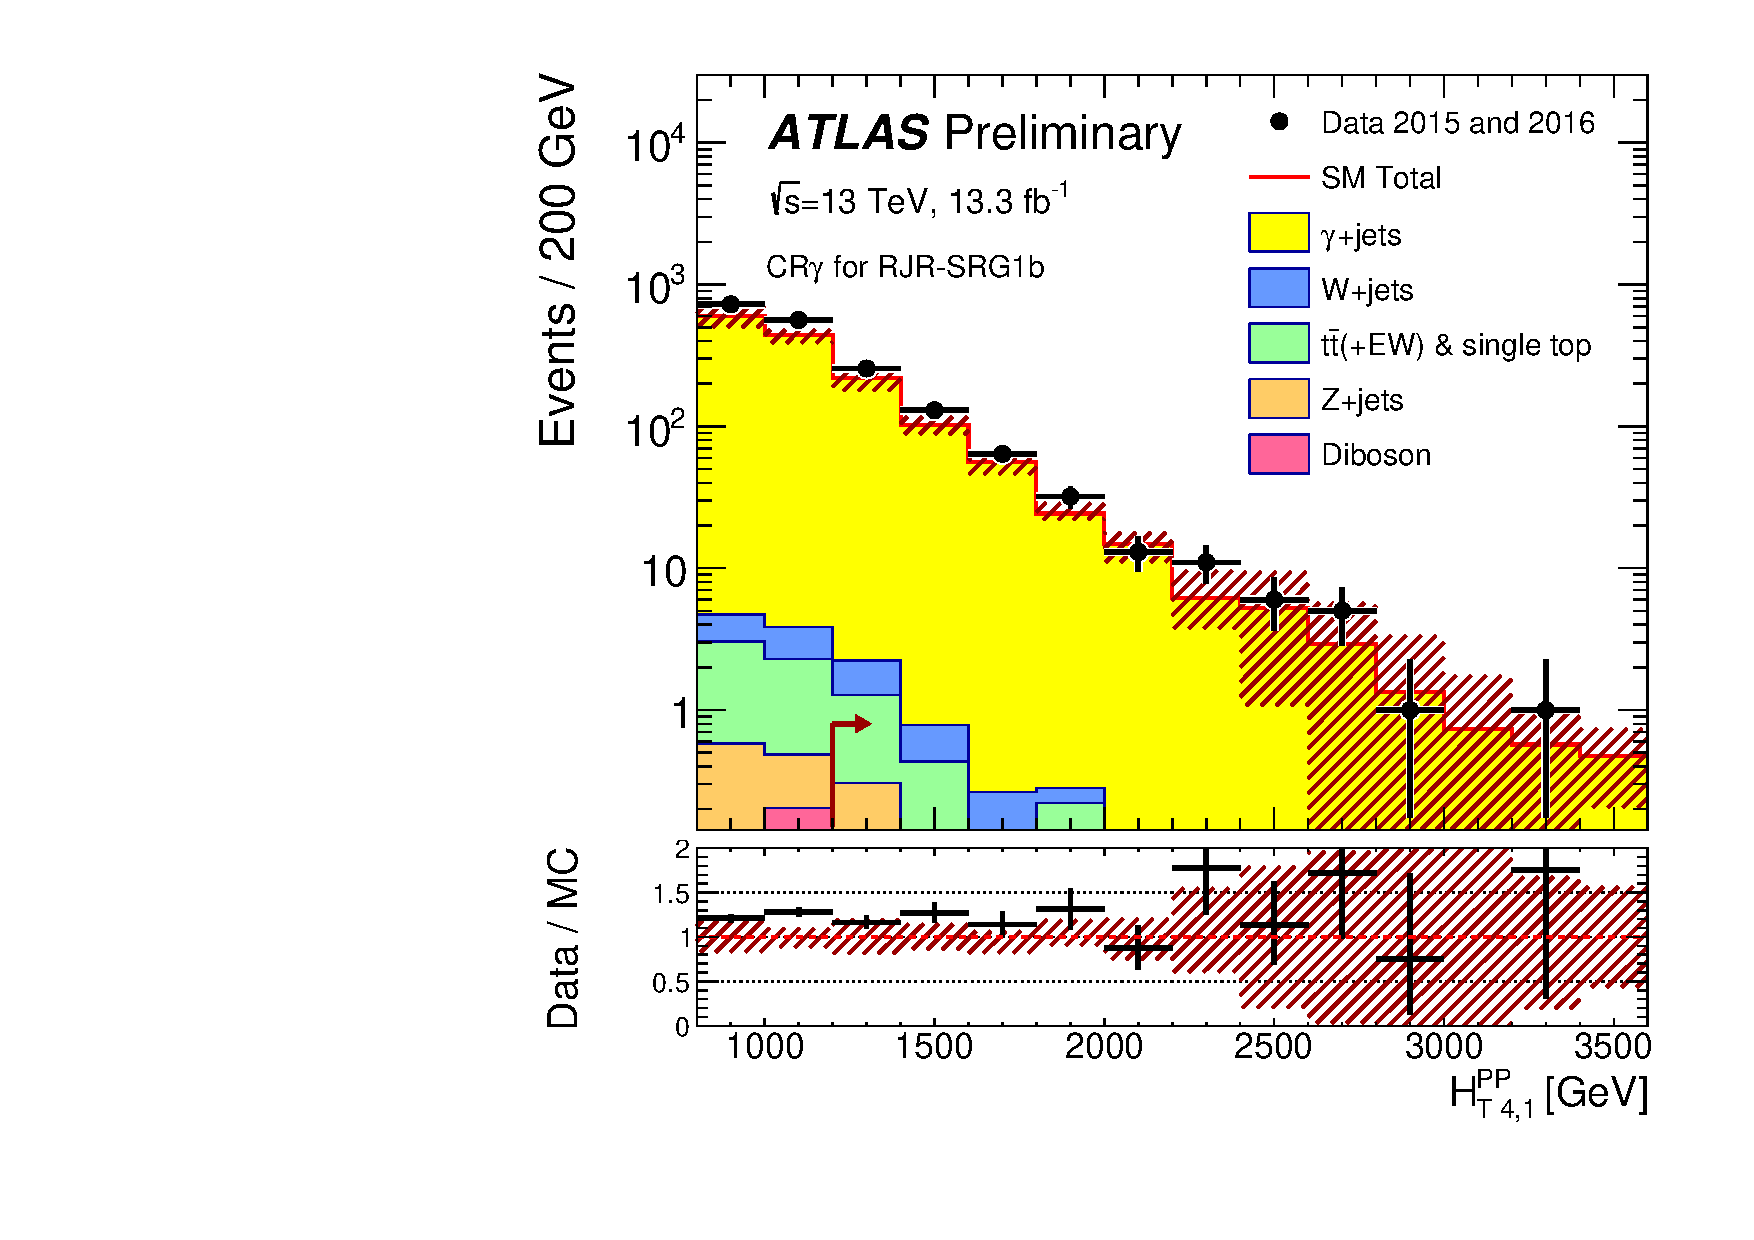
\includegraphics[width=0.45\textwidth]{figures/ATLAS-CONF-2016-078_INT/N-1Plots/AtlasStyle/Preliminary/CRY_SRJigsawSRG1b_LastCut_CRY_minusone}
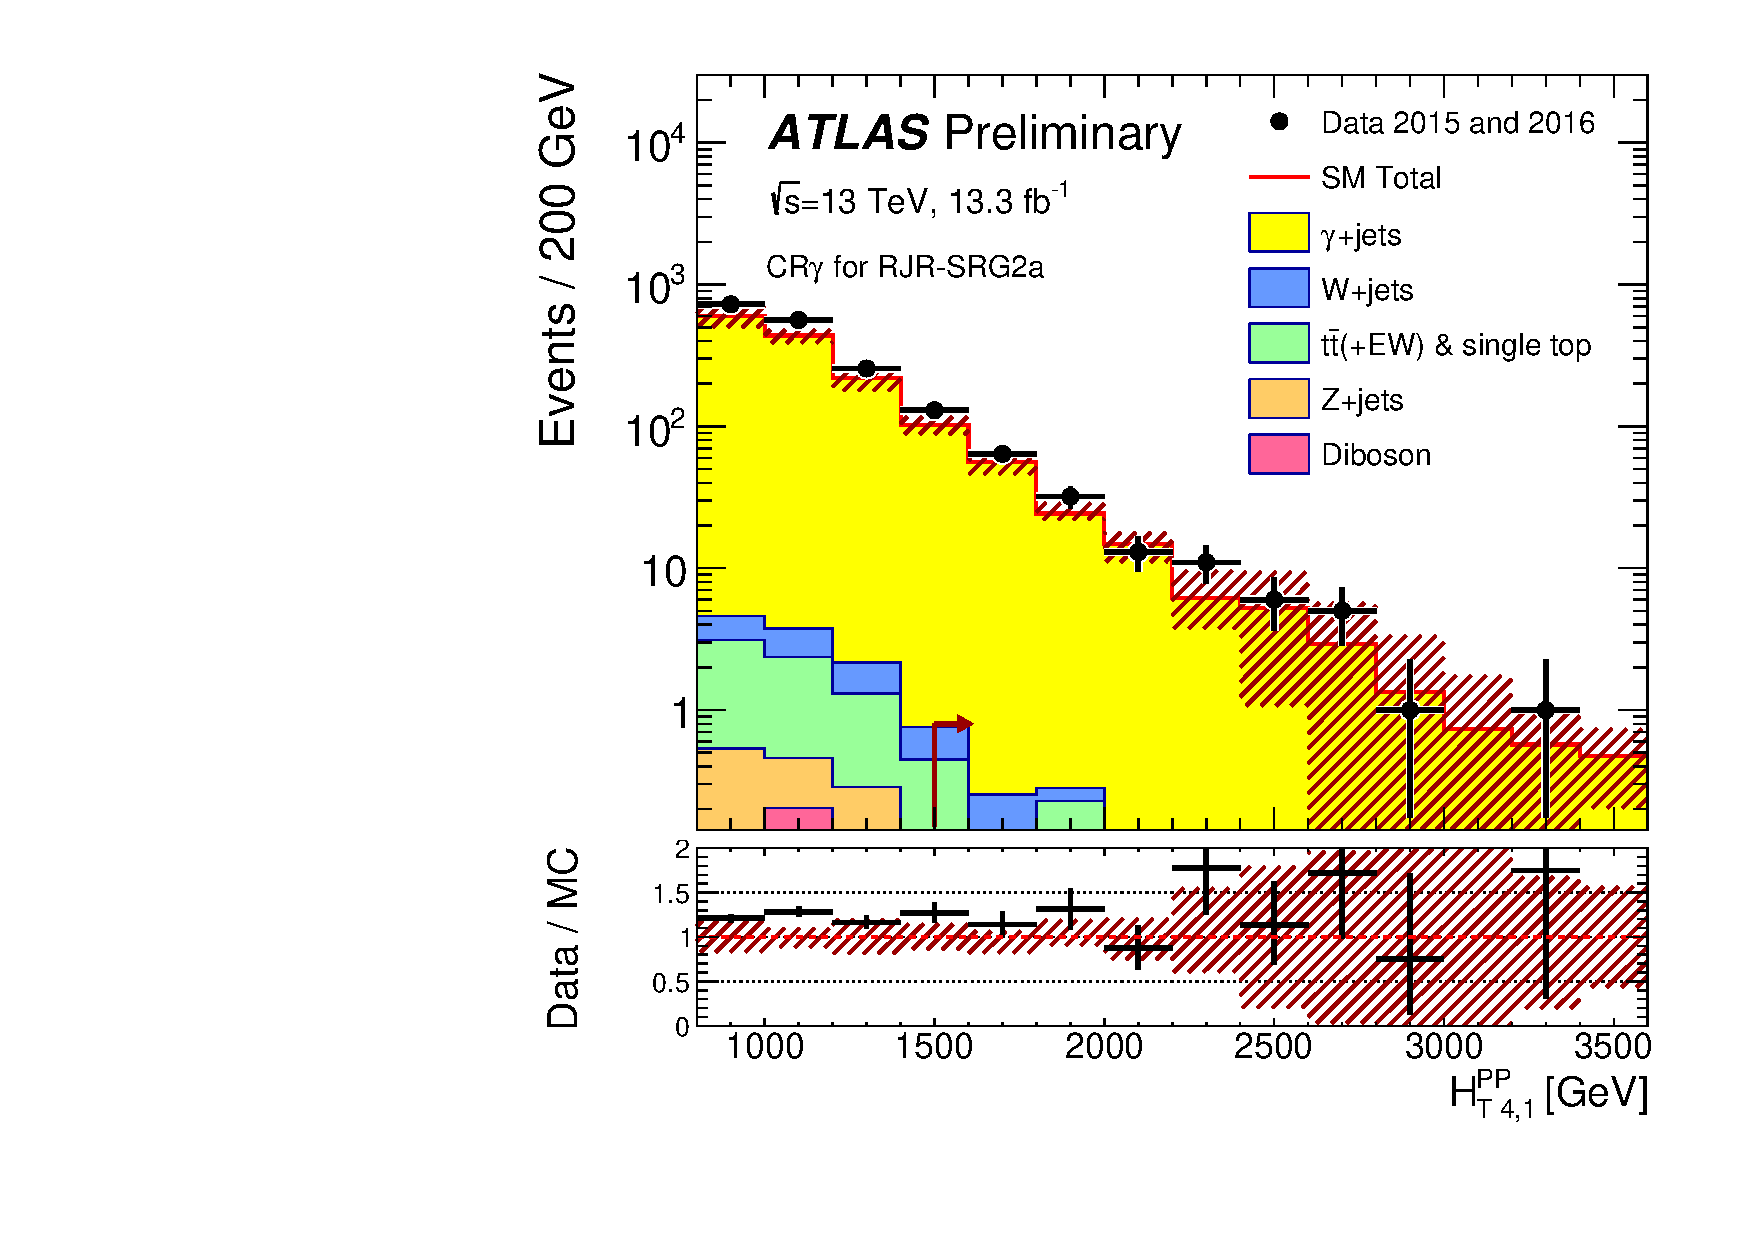
\includegraphics[width=0.45\textwidth]{figures/ATLAS-CONF-2016-078_INT/N-1Plots/AtlasStyle/Preliminary/CRY_SRJigsawSRG2a_LastCut_CRY_minusone}
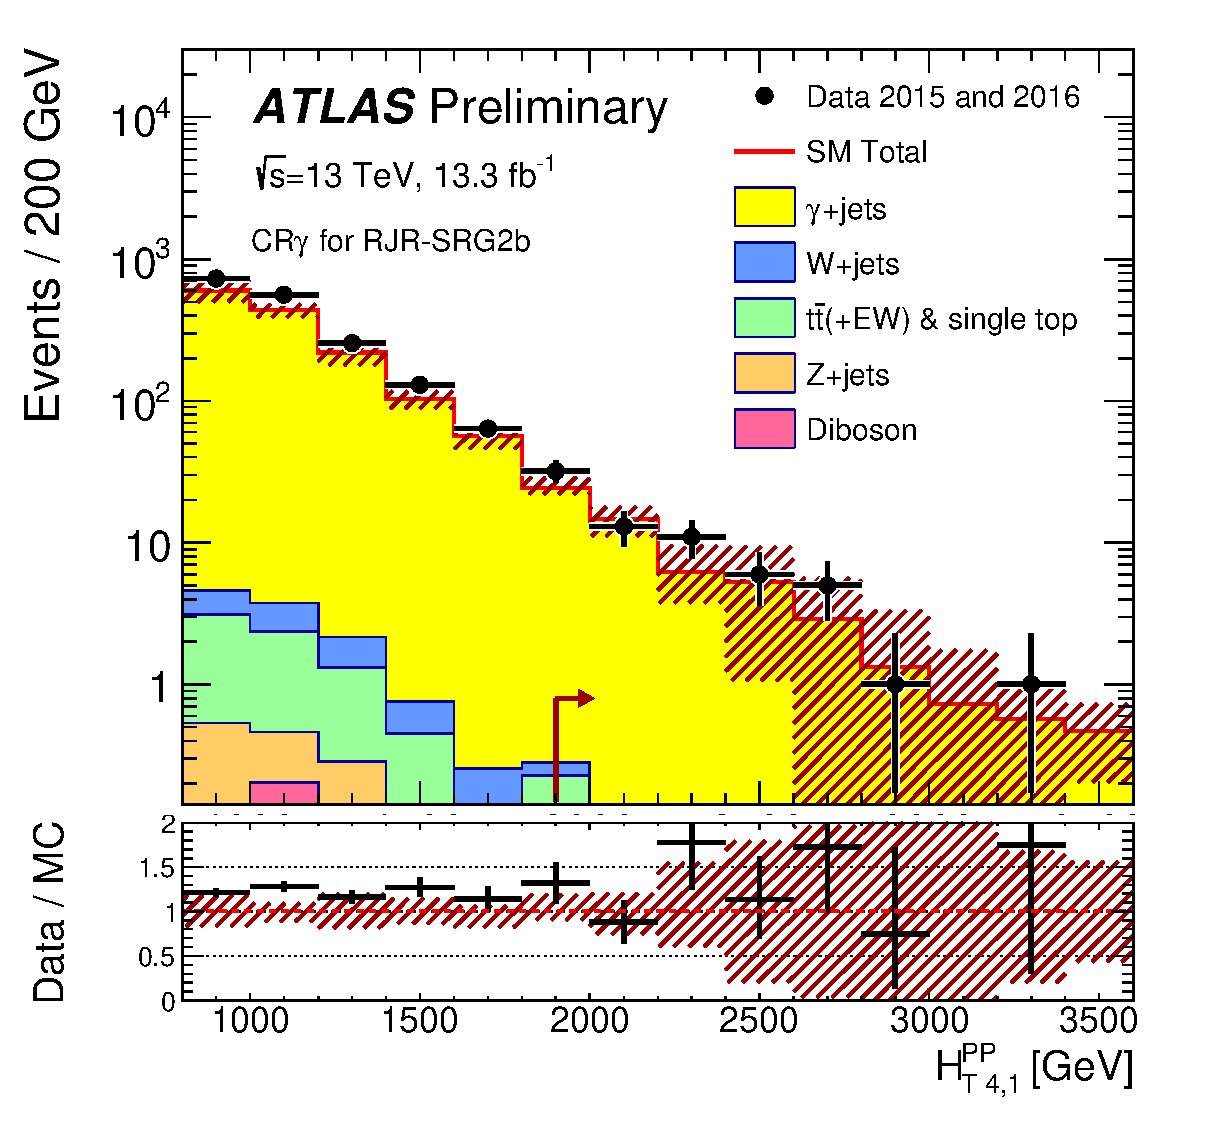
\includegraphics[width=0.45\textwidth]{figures/ATLAS-CONF-2016-078_INT/N-1Plots/AtlasStyle/Preliminary/CRY_SRJigsawSRG2b_LastCut_CRY_minusone}
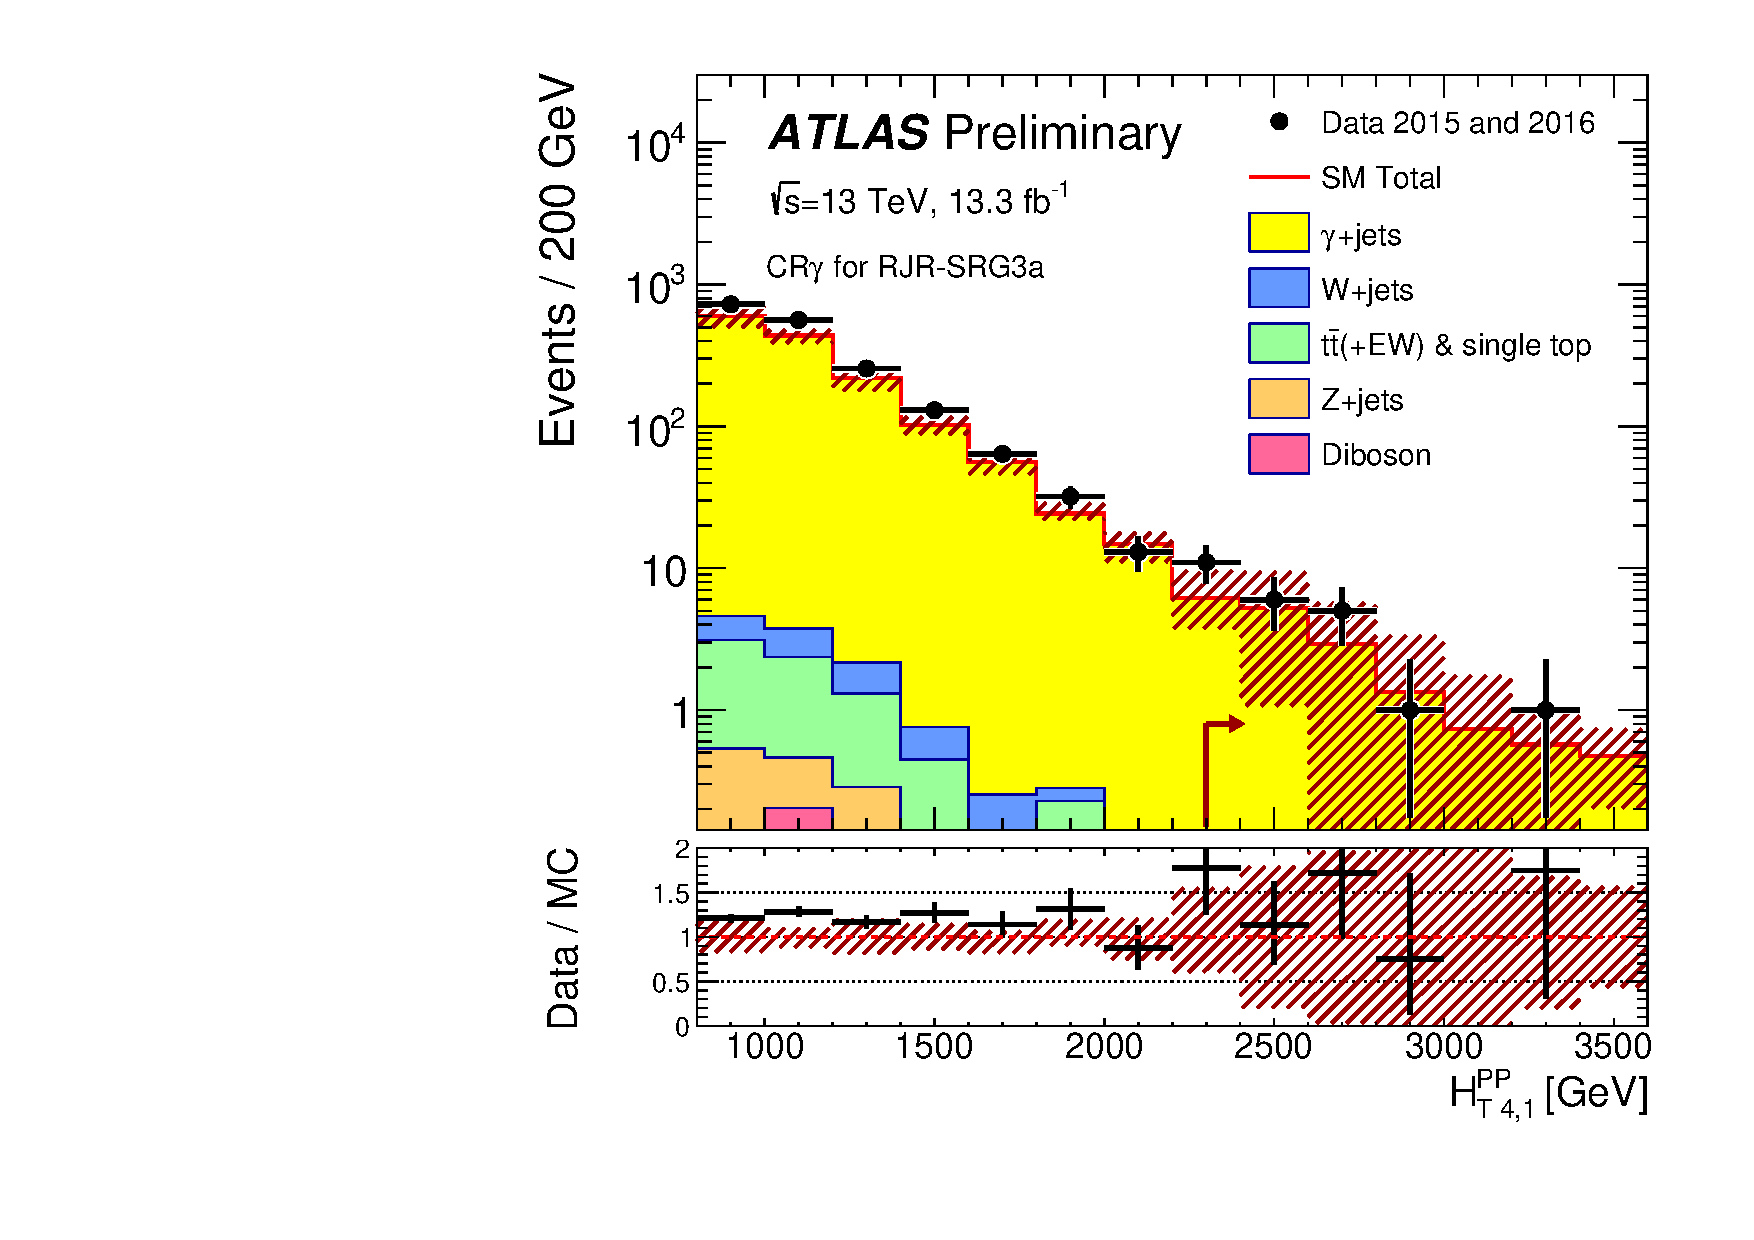
\includegraphics[width=0.45\textwidth]{figures/ATLAS-CONF-2016-078_INT/N-1Plots/AtlasStyle/Preliminary/CRY_SRJigsawSRG3a_LastCut_CRY_minusone}
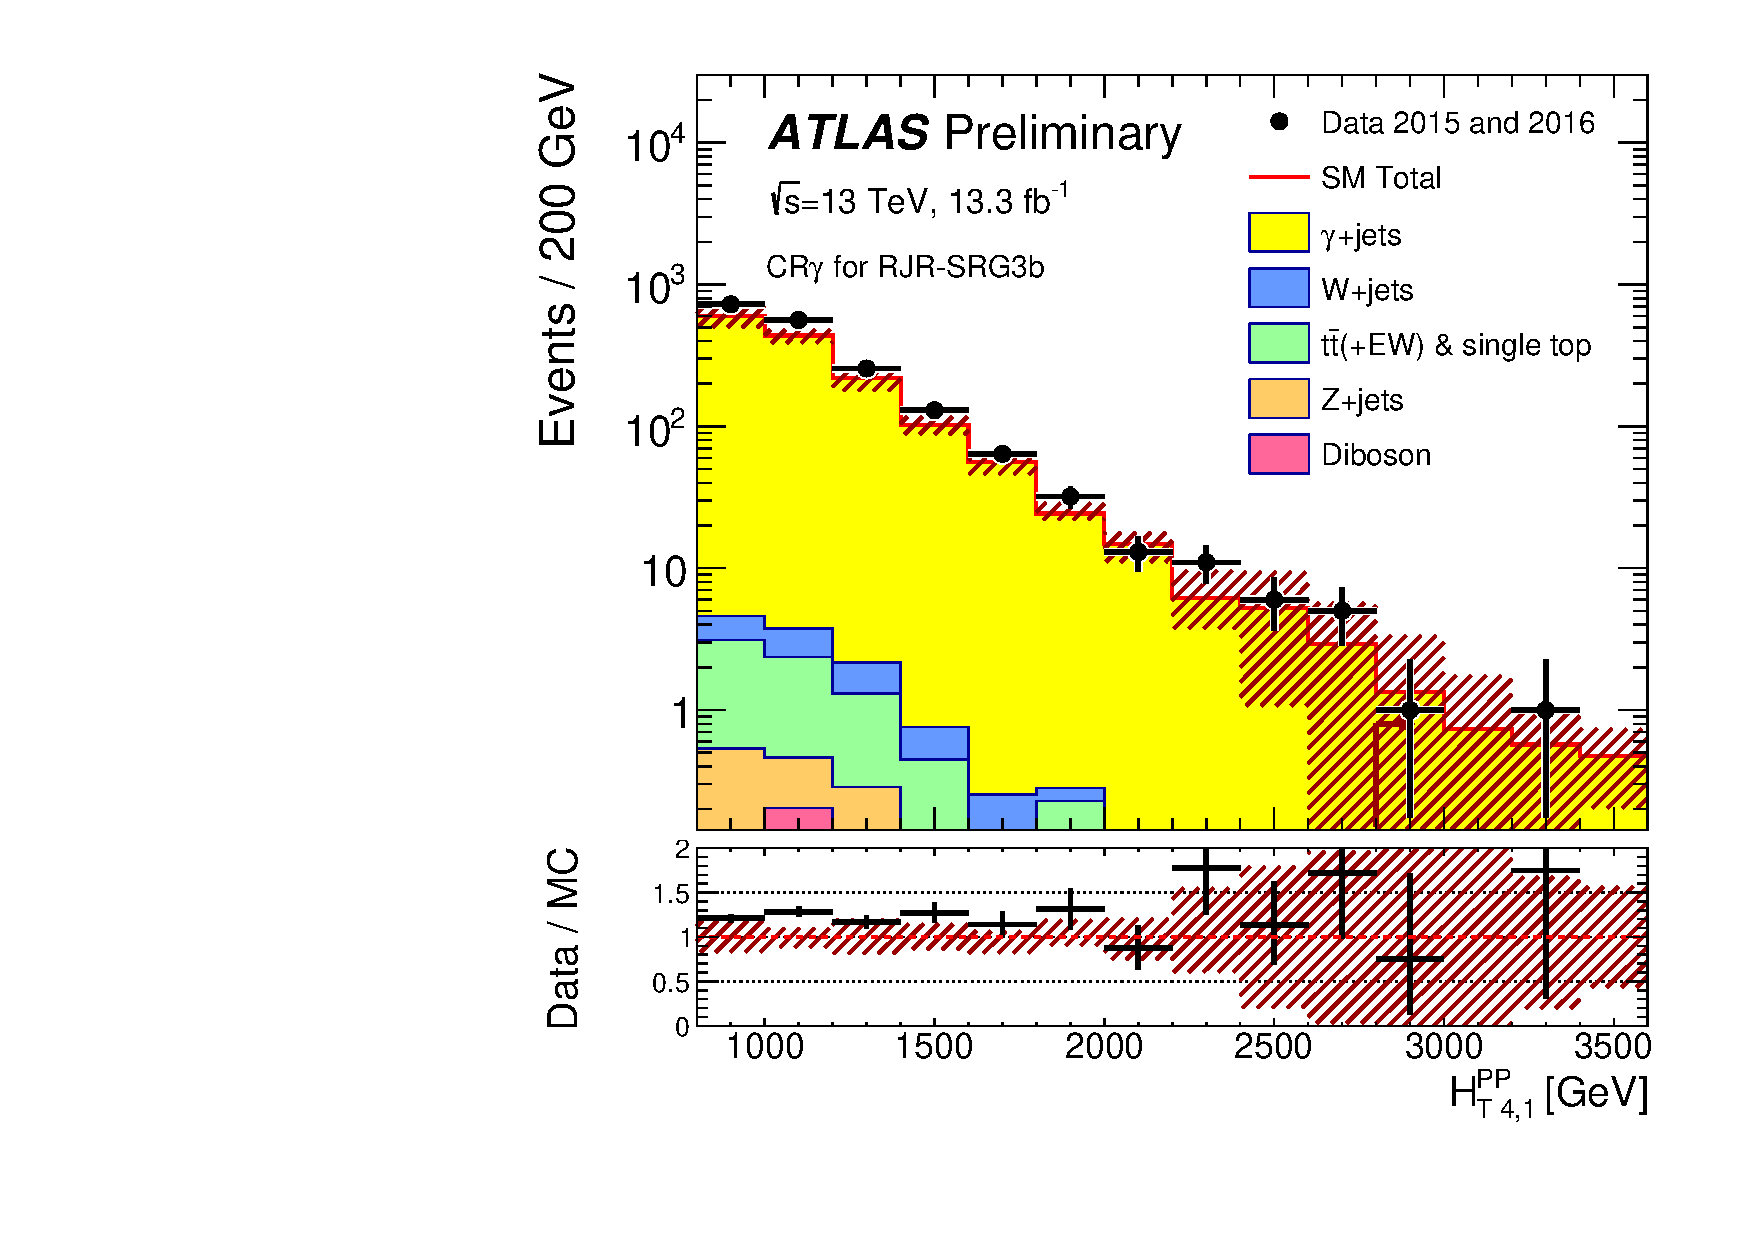
\includegraphics[width=0.45\textwidth]{figures/ATLAS-CONF-2016-078_INT/N-1Plots/AtlasStyle/Preliminary/CRY_SRJigsawSRG3b_LastCut_CRY_minusone}
\end{center}
\caption{Scale variable distributions for the gluino CRY regions.}
\label{fig:CRY_SRJigsawSRG1a_LastCut_CRY_minusone}
\end{figure}

\clearpage
\begin{figure}[tbph]
\begin{center}
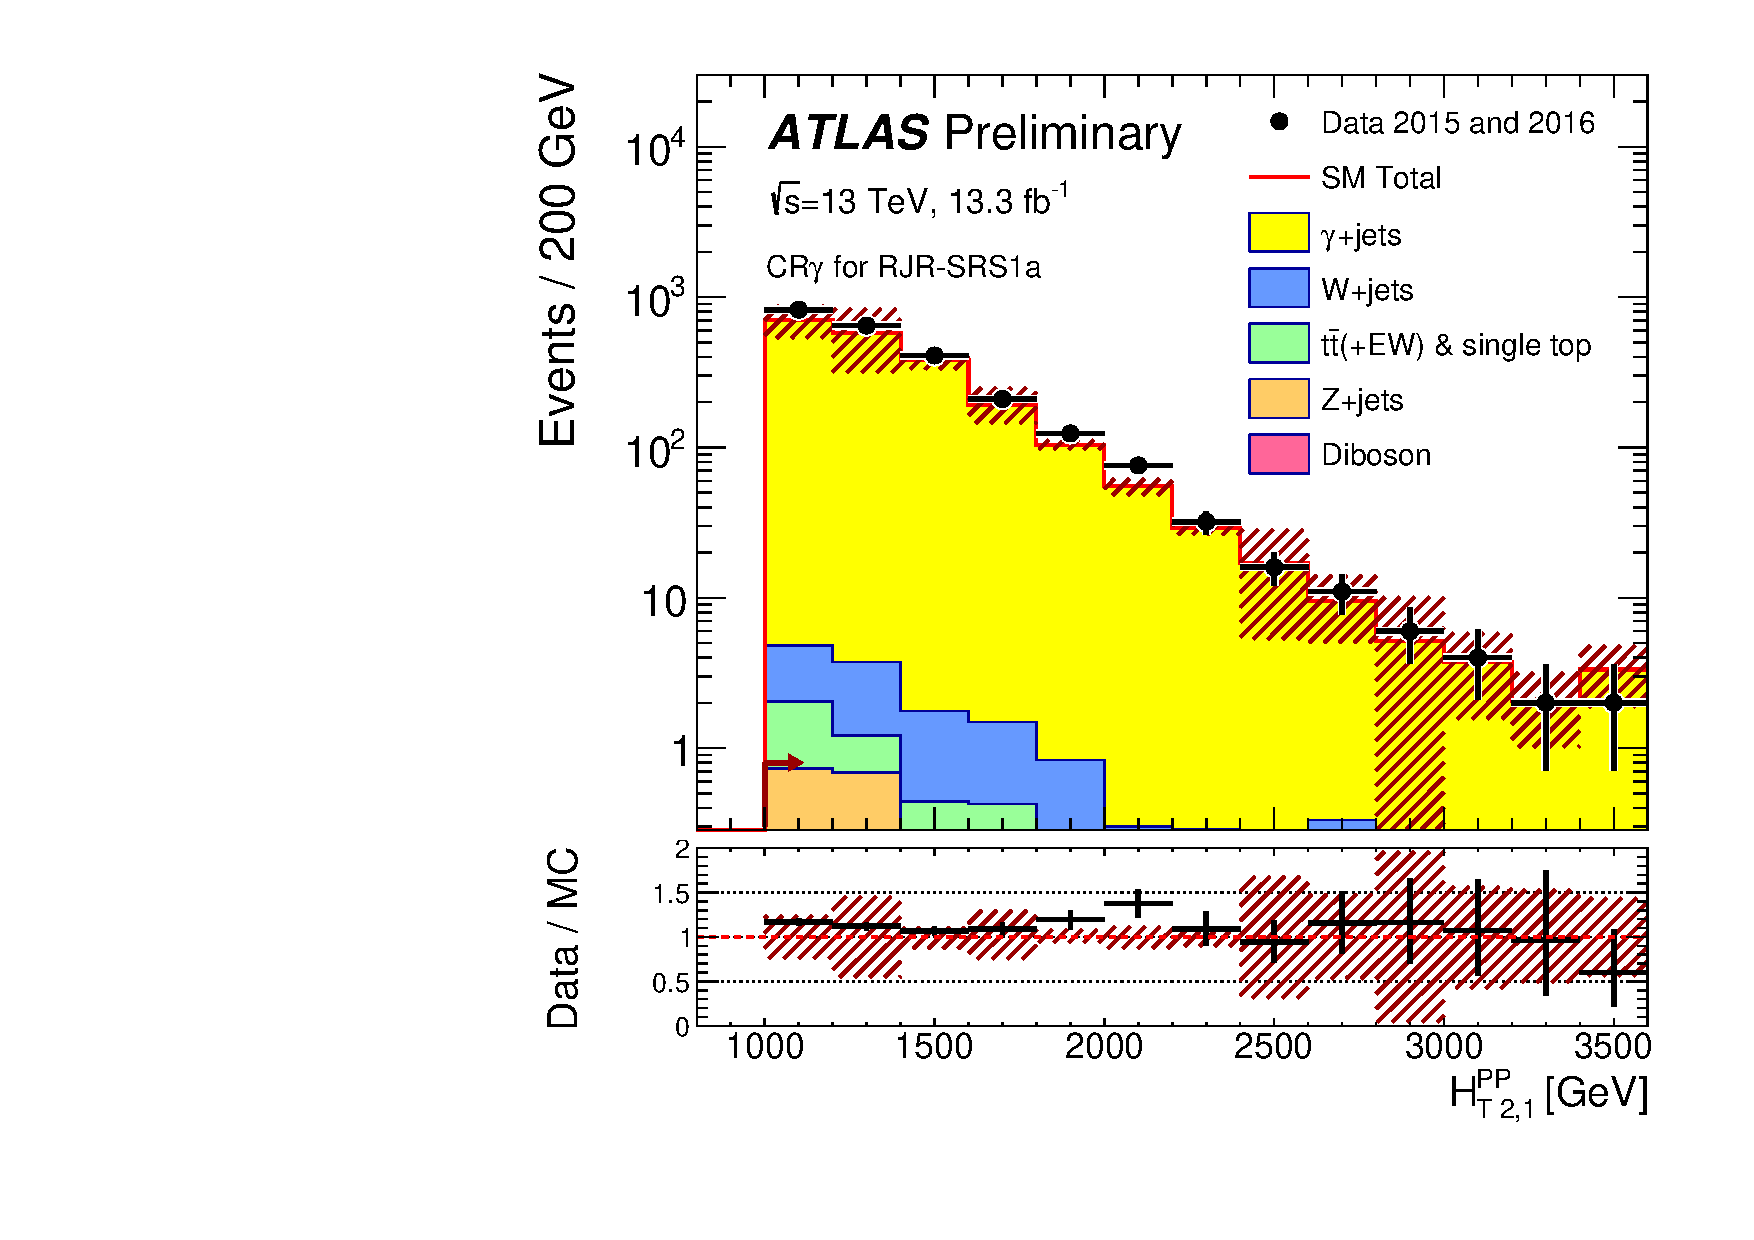
\includegraphics[width=0.45\textwidth]{figures/ATLAS-CONF-2016-078_INT/N-1Plots/AtlasStyle/Preliminary/CRY_SRJigsawSRS1a_LastCut_CRY_minusone}
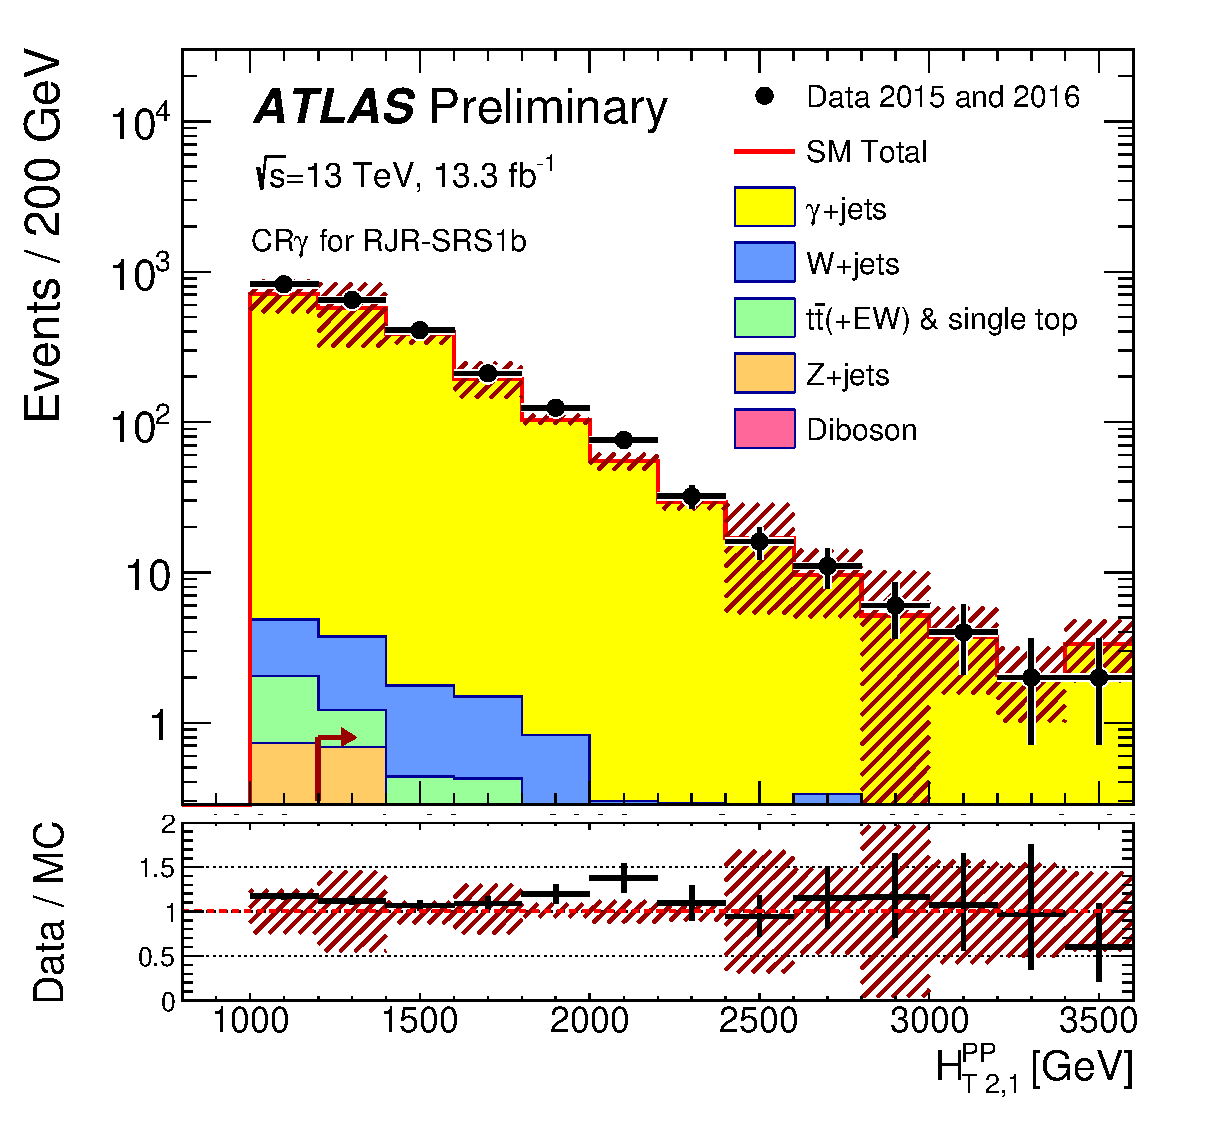
\includegraphics[width=0.45\textwidth]{figures/ATLAS-CONF-2016-078_INT/N-1Plots/AtlasStyle/Preliminary/CRY_SRJigsawSRS1b_LastCut_CRY_minusone}
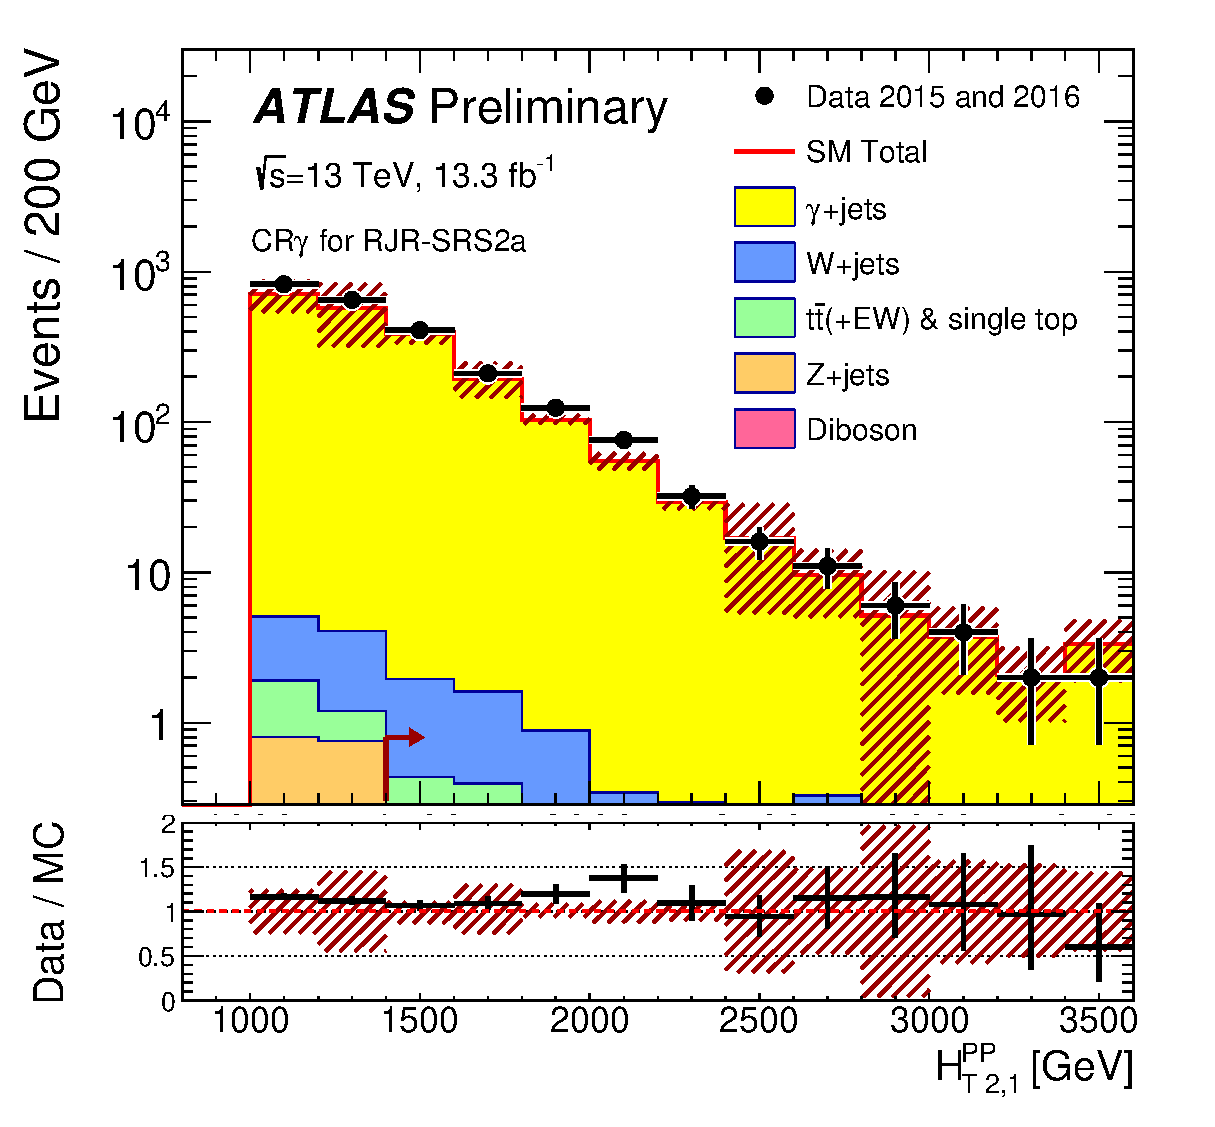
\includegraphics[width=0.45\textwidth]{figures/ATLAS-CONF-2016-078_INT/N-1Plots/AtlasStyle/Preliminary/CRY_SRJigsawSRS2a_LastCut_CRY_minusone}
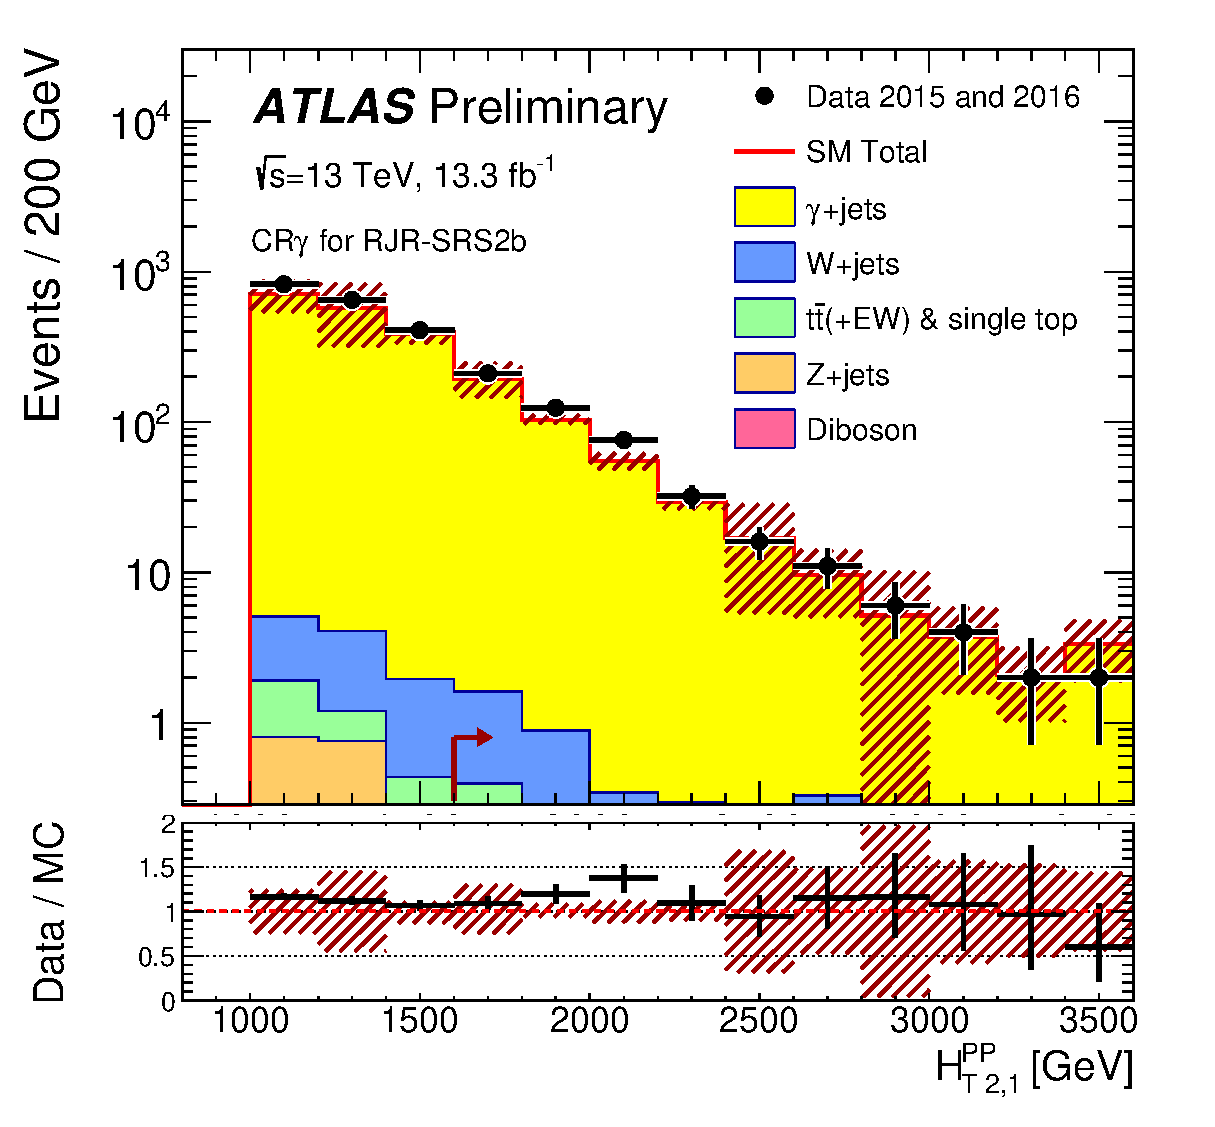
\includegraphics[width=0.45\textwidth]{figures/ATLAS-CONF-2016-078_INT/N-1Plots/AtlasStyle/Preliminary/CRY_SRJigsawSRS2b_LastCut_CRY_minusone}
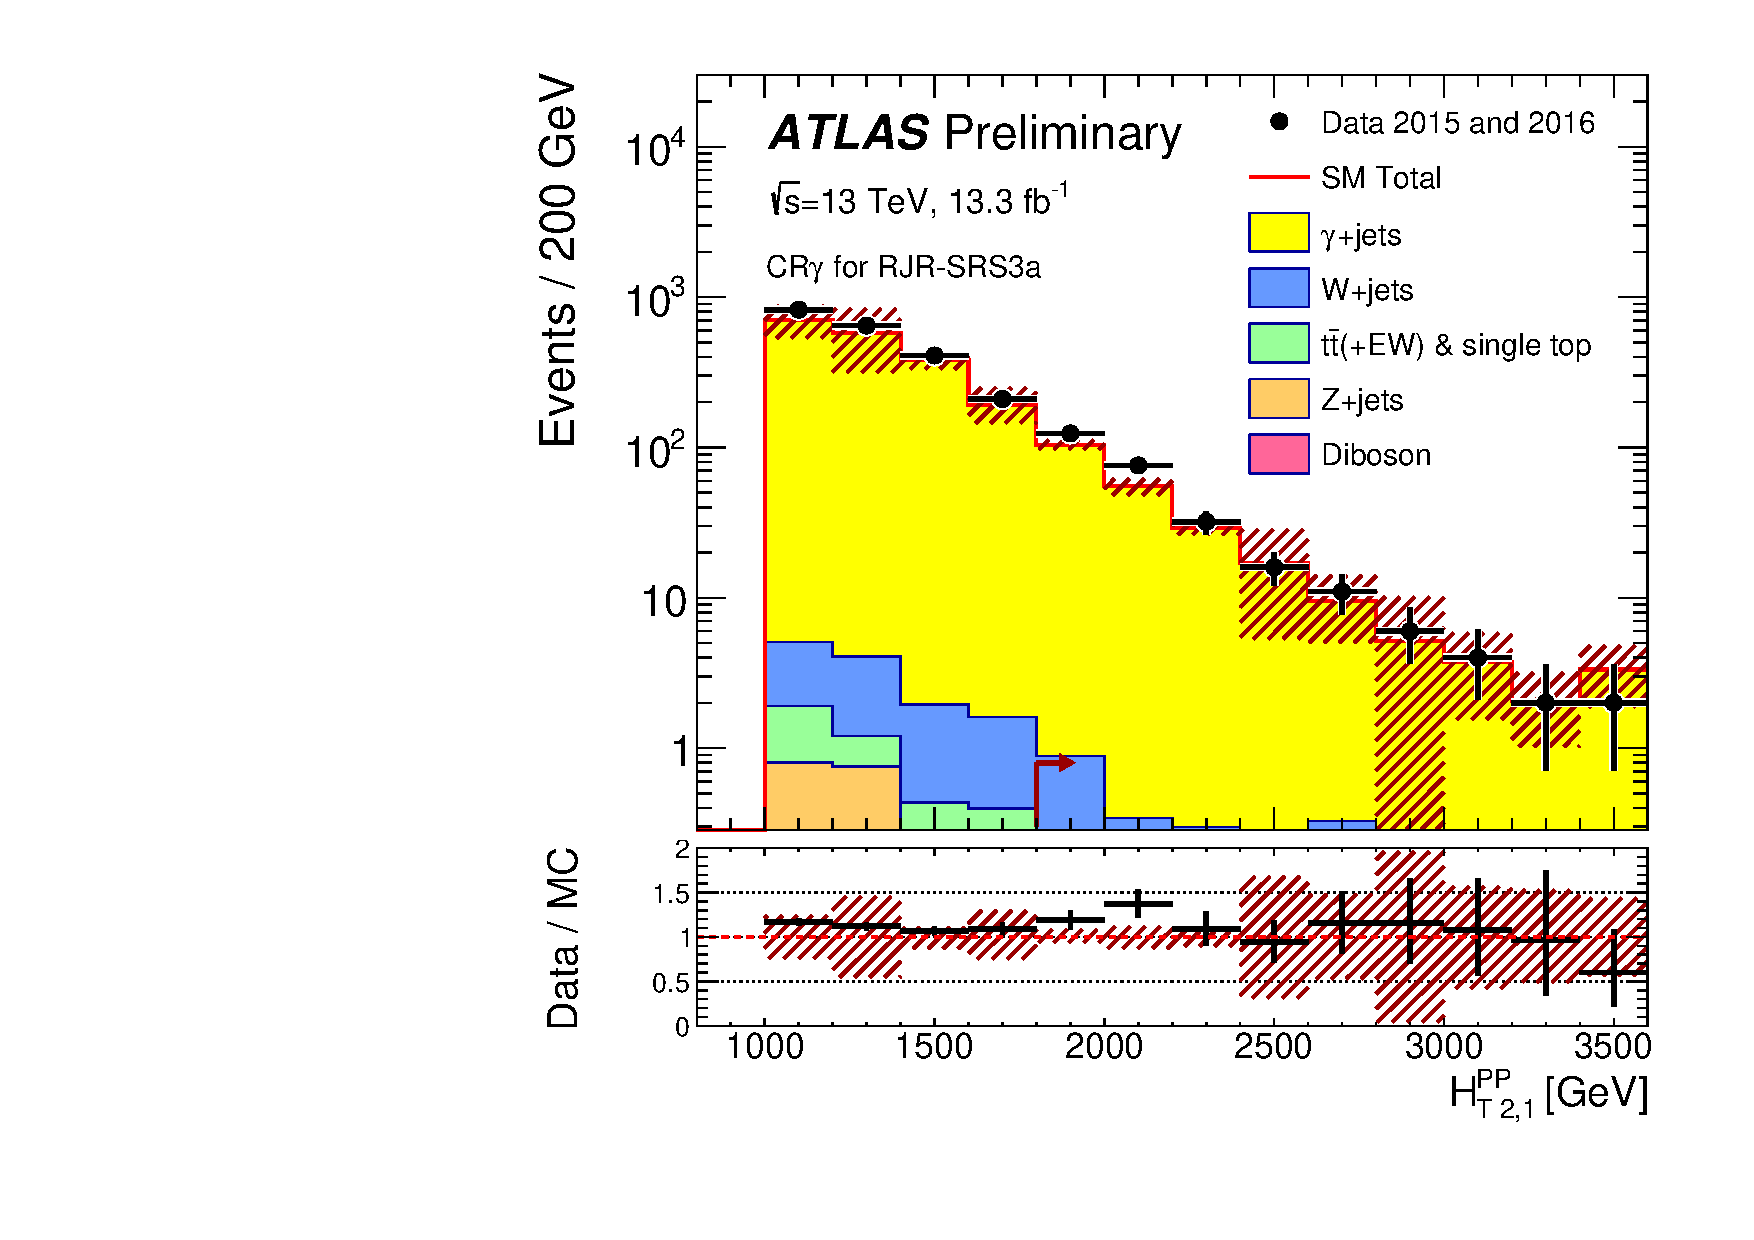
\includegraphics[width=0.45\textwidth]{figures/ATLAS-CONF-2016-078_INT/N-1Plots/AtlasStyle/Preliminary/CRY_SRJigsawSRS3a_LastCut_CRY_minusone}
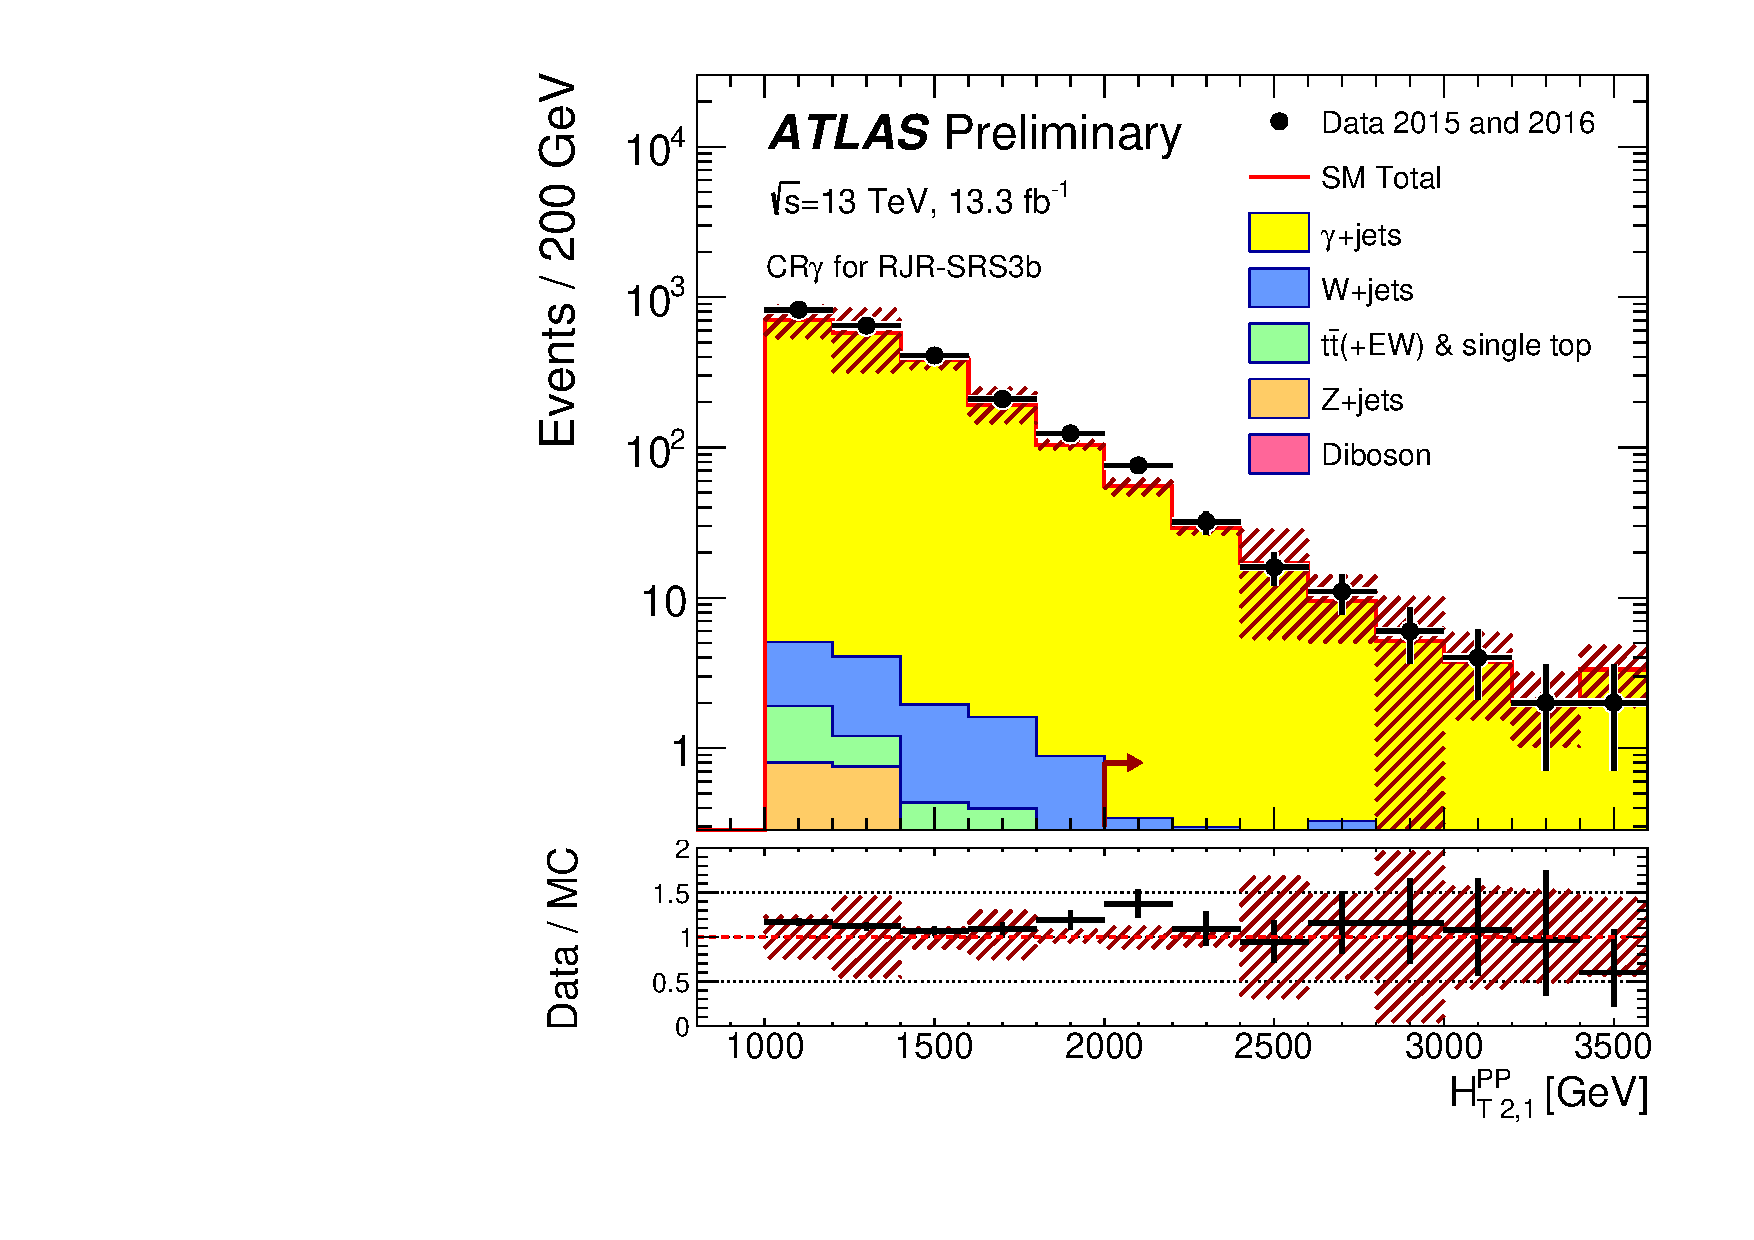
\includegraphics[width=0.45\textwidth]{figures/ATLAS-CONF-2016-078_INT/N-1Plots/AtlasStyle/Preliminary/CRY_SRJigsawSRS3b_LastCut_CRY_minusone}
\end{center}
\caption{Scale variable distributions for the squark CRY regions.}
\label{fig:CRY_SRJigsawSRS1a_LastCut_CRY_minusone}
\end{figure}

\clearpage
\begin{figure}[tbph]
\begin{center}
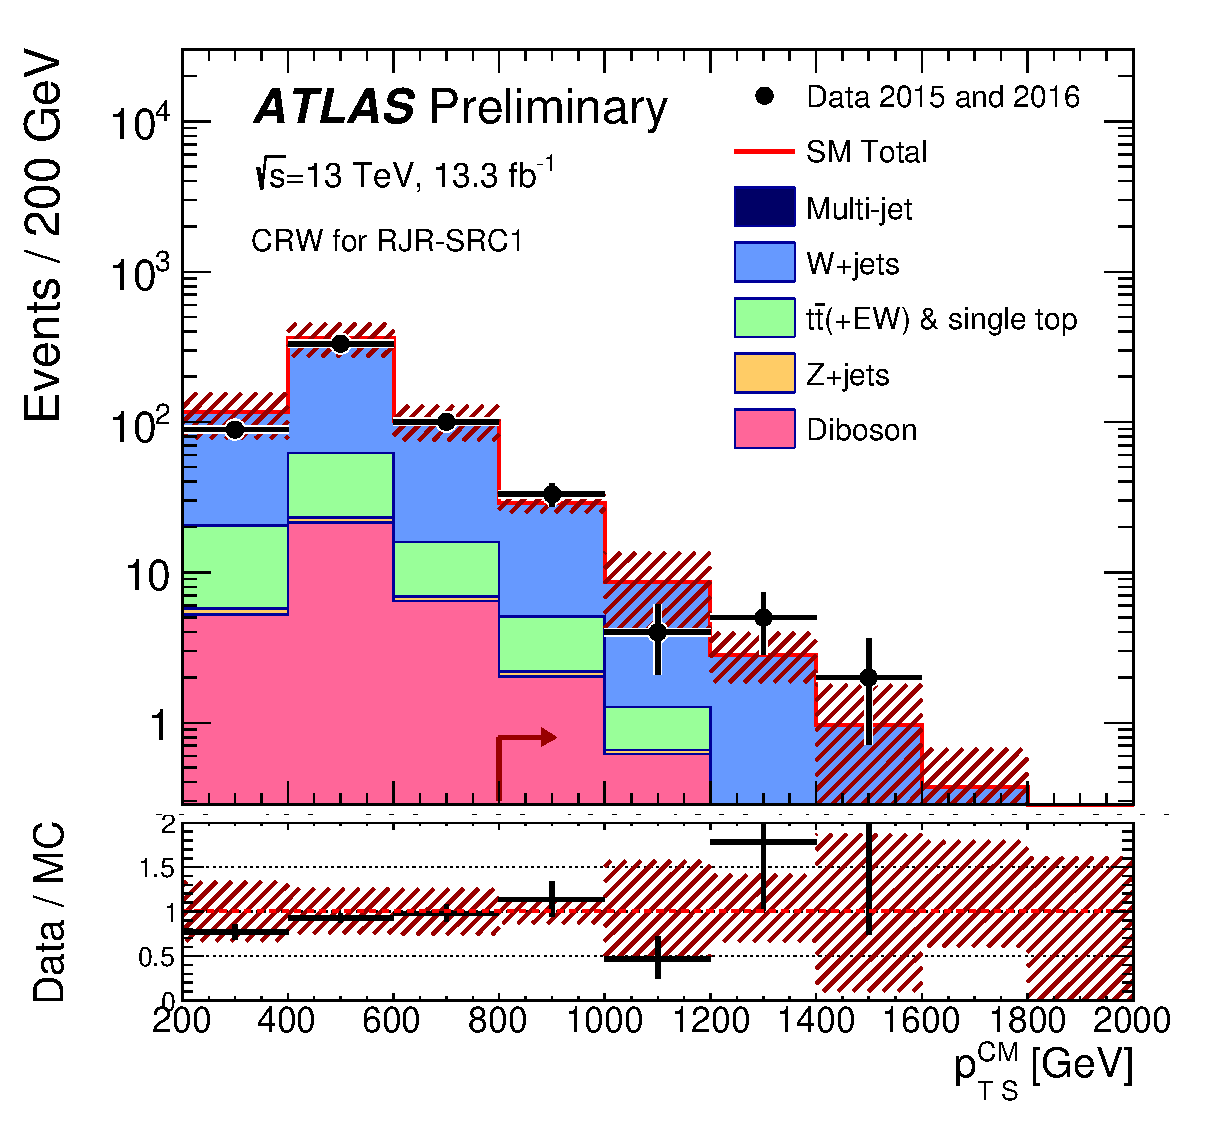
\includegraphics[width=0.45\textwidth]{figures/ATLAS-CONF-2016-078_INT/N-1Plots/AtlasStyle/Preliminary/CRW_SRJigsawSRC1_LastCut_CRW_minusone}
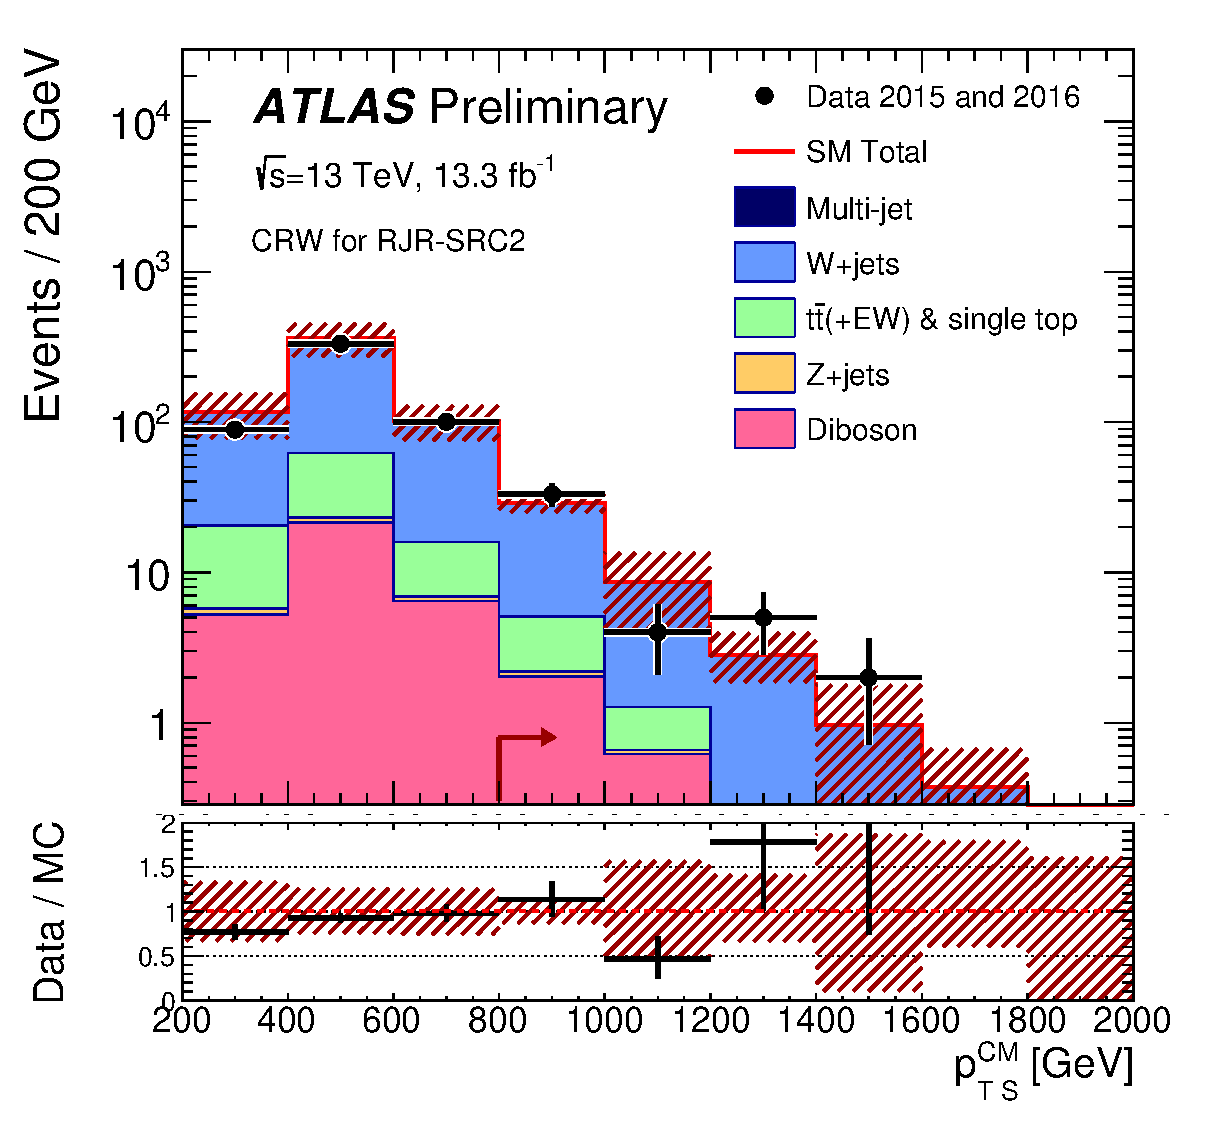
\includegraphics[width=0.45\textwidth]{figures/ATLAS-CONF-2016-078_INT/N-1Plots/AtlasStyle/Preliminary/CRW_SRJigsawSRC2_LastCut_CRW_minusone}
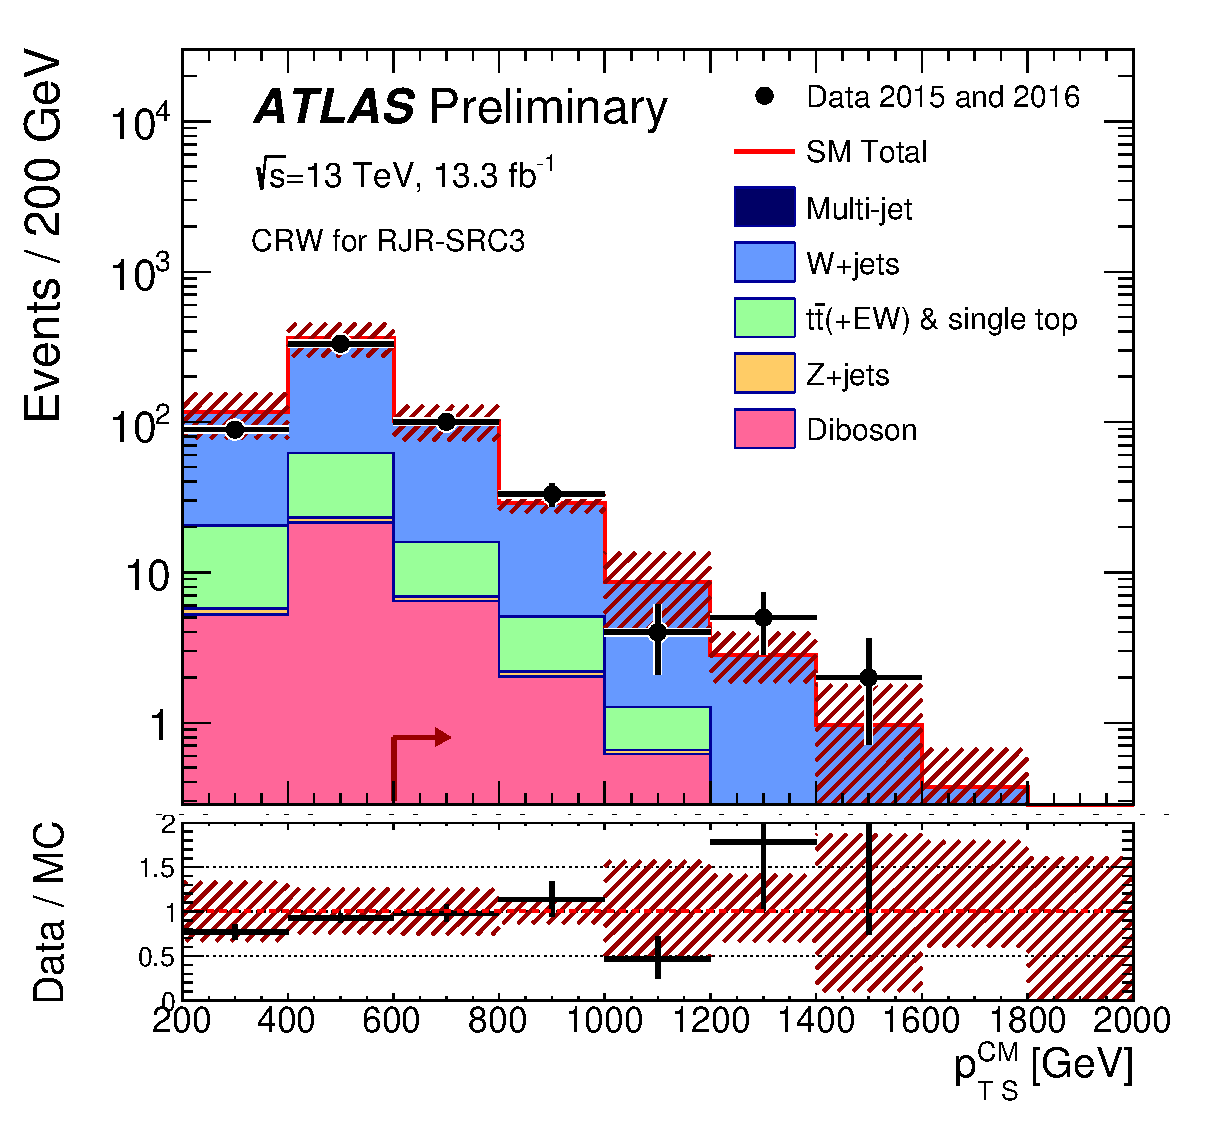
\includegraphics[width=0.45\textwidth]{figures/ATLAS-CONF-2016-078_INT/N-1Plots/AtlasStyle/Preliminary/CRW_SRJigsawSRC3_LastCut_CRW_minusone}
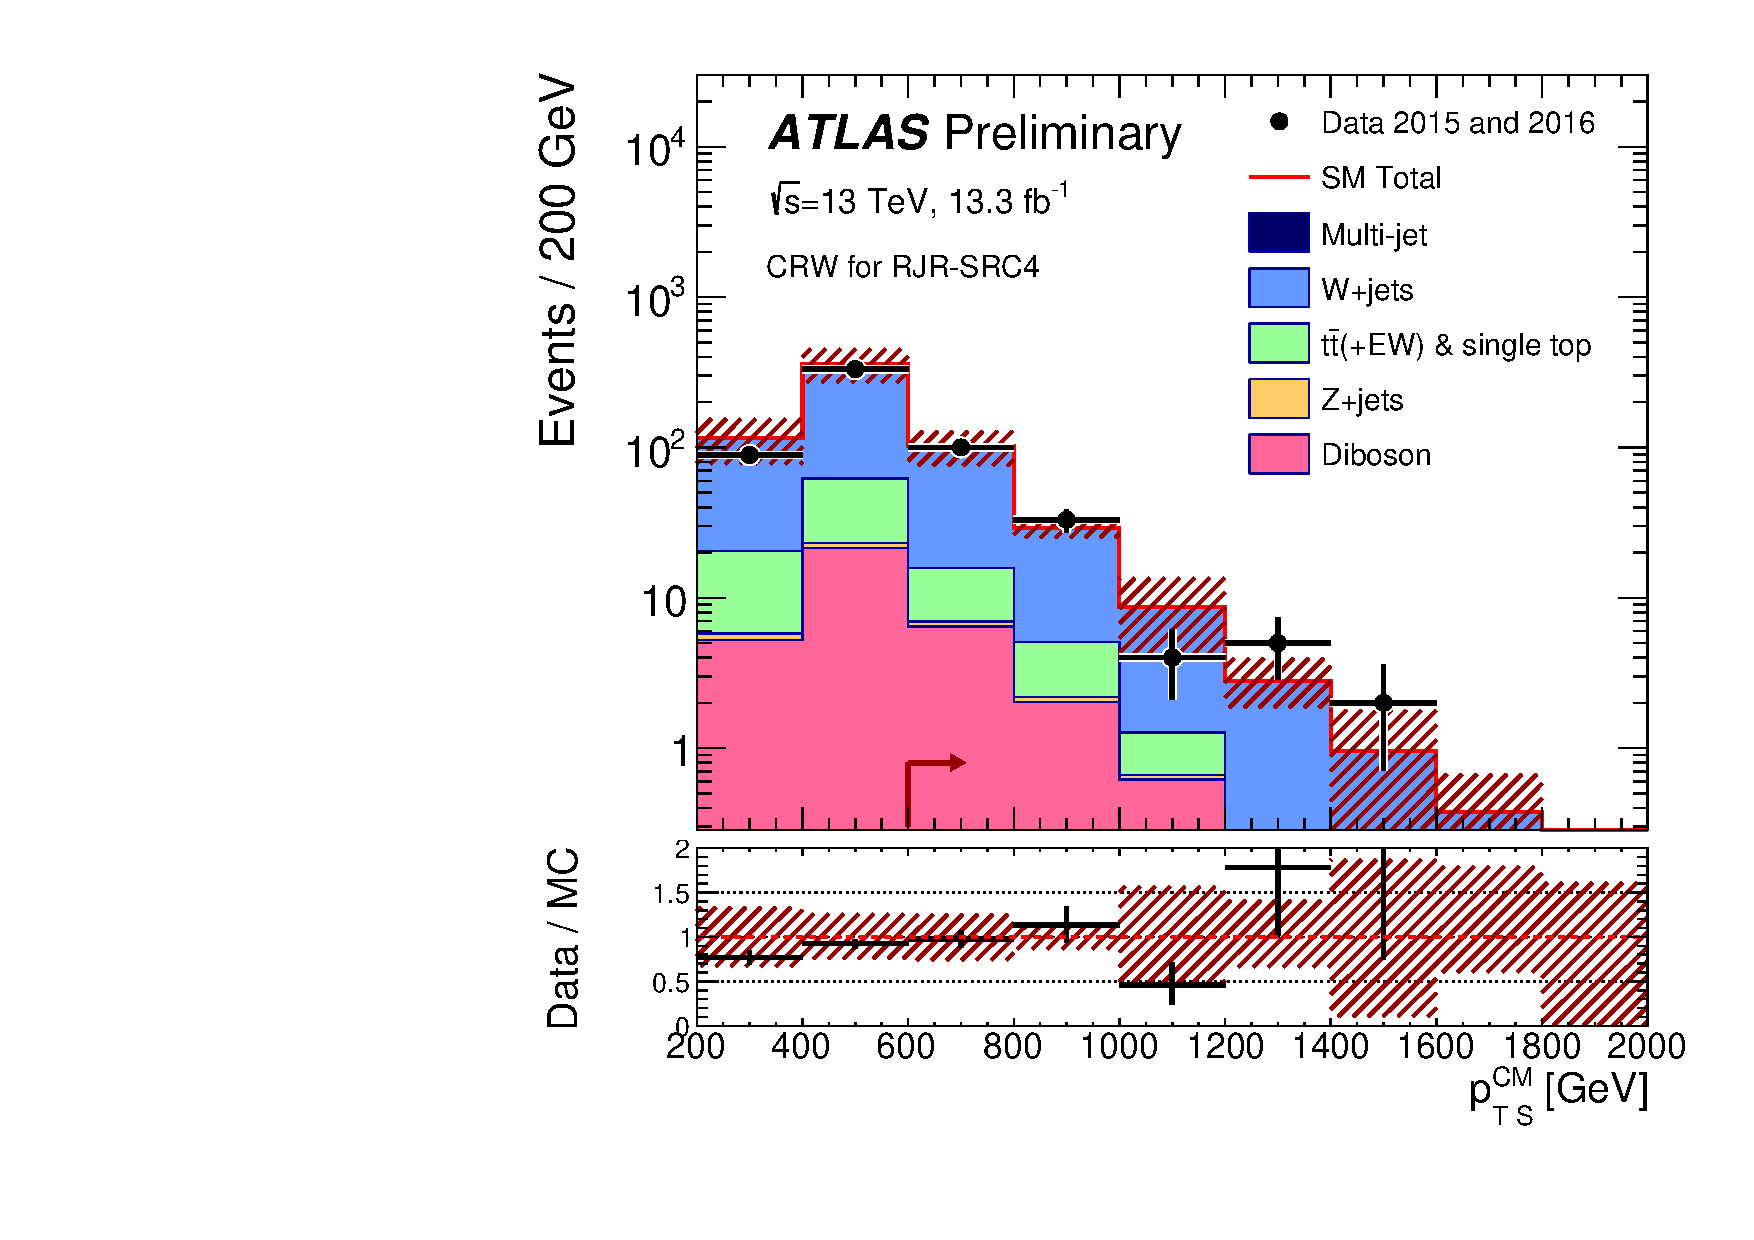
\includegraphics[width=0.45\textwidth]{figures/ATLAS-CONF-2016-078_INT/N-1Plots/AtlasStyle/Preliminary/CRW_SRJigsawSRC4_LastCut_CRW_minusone}
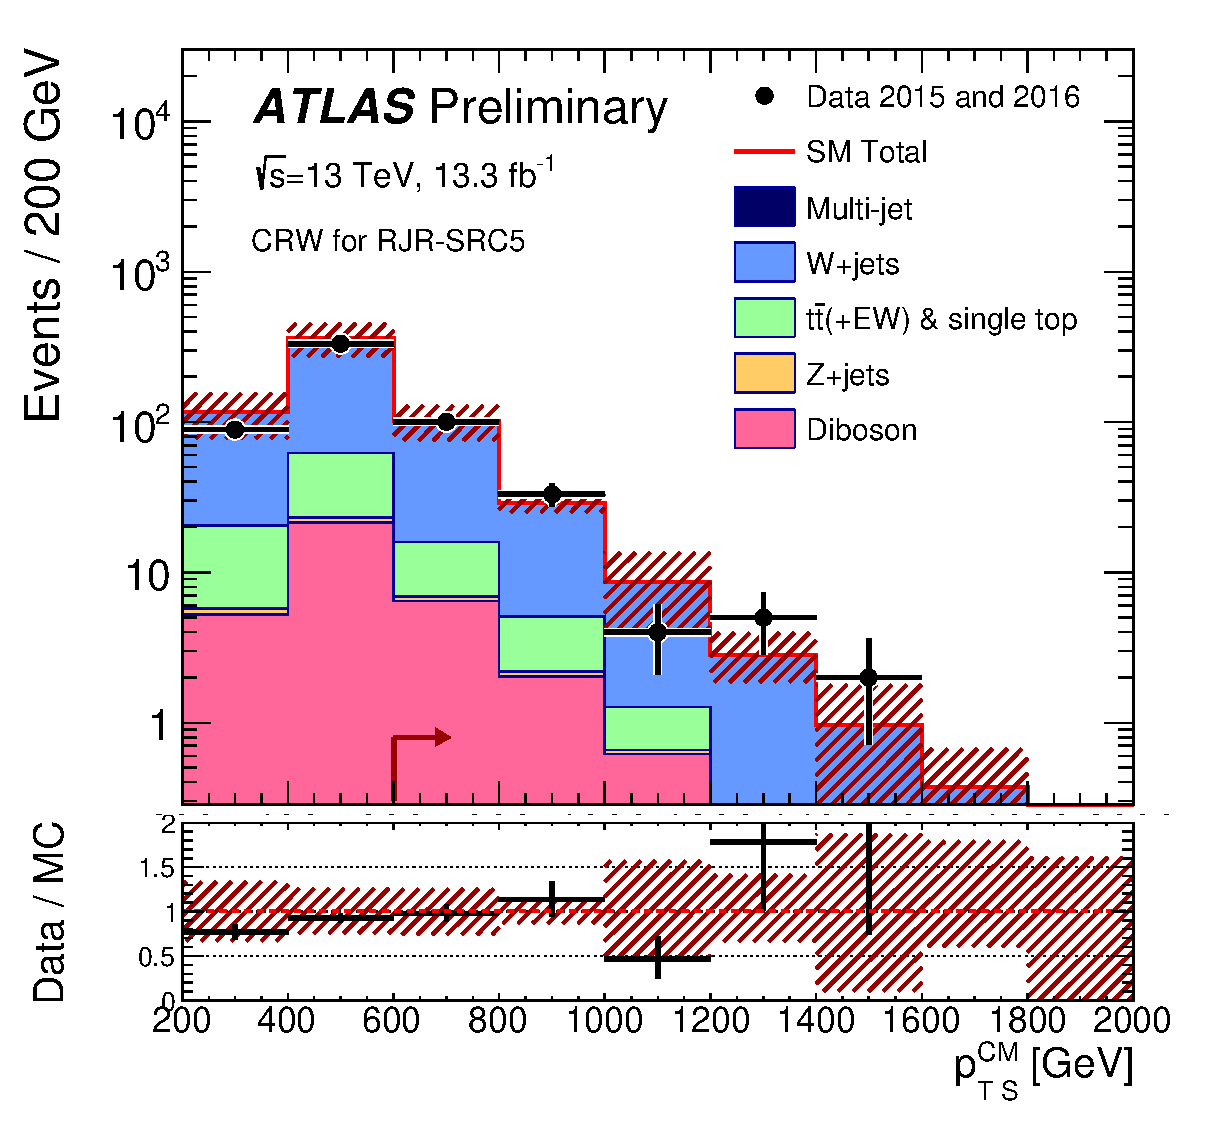
\includegraphics[width=0.45\textwidth]{figures/ATLAS-CONF-2016-078_INT/N-1Plots/AtlasStyle/Preliminary/CRW_SRJigsawSRC5_LastCut_CRW_minusone}
\end{center}
\caption{Scale variable distributions for the compressed CRW regions.}
\label{fig:CRW_SRJigsawSRC1_LastCut_CRW_minusone}
\end{figure}

\clearpage
\begin{figure}[tbph]
\begin{center}
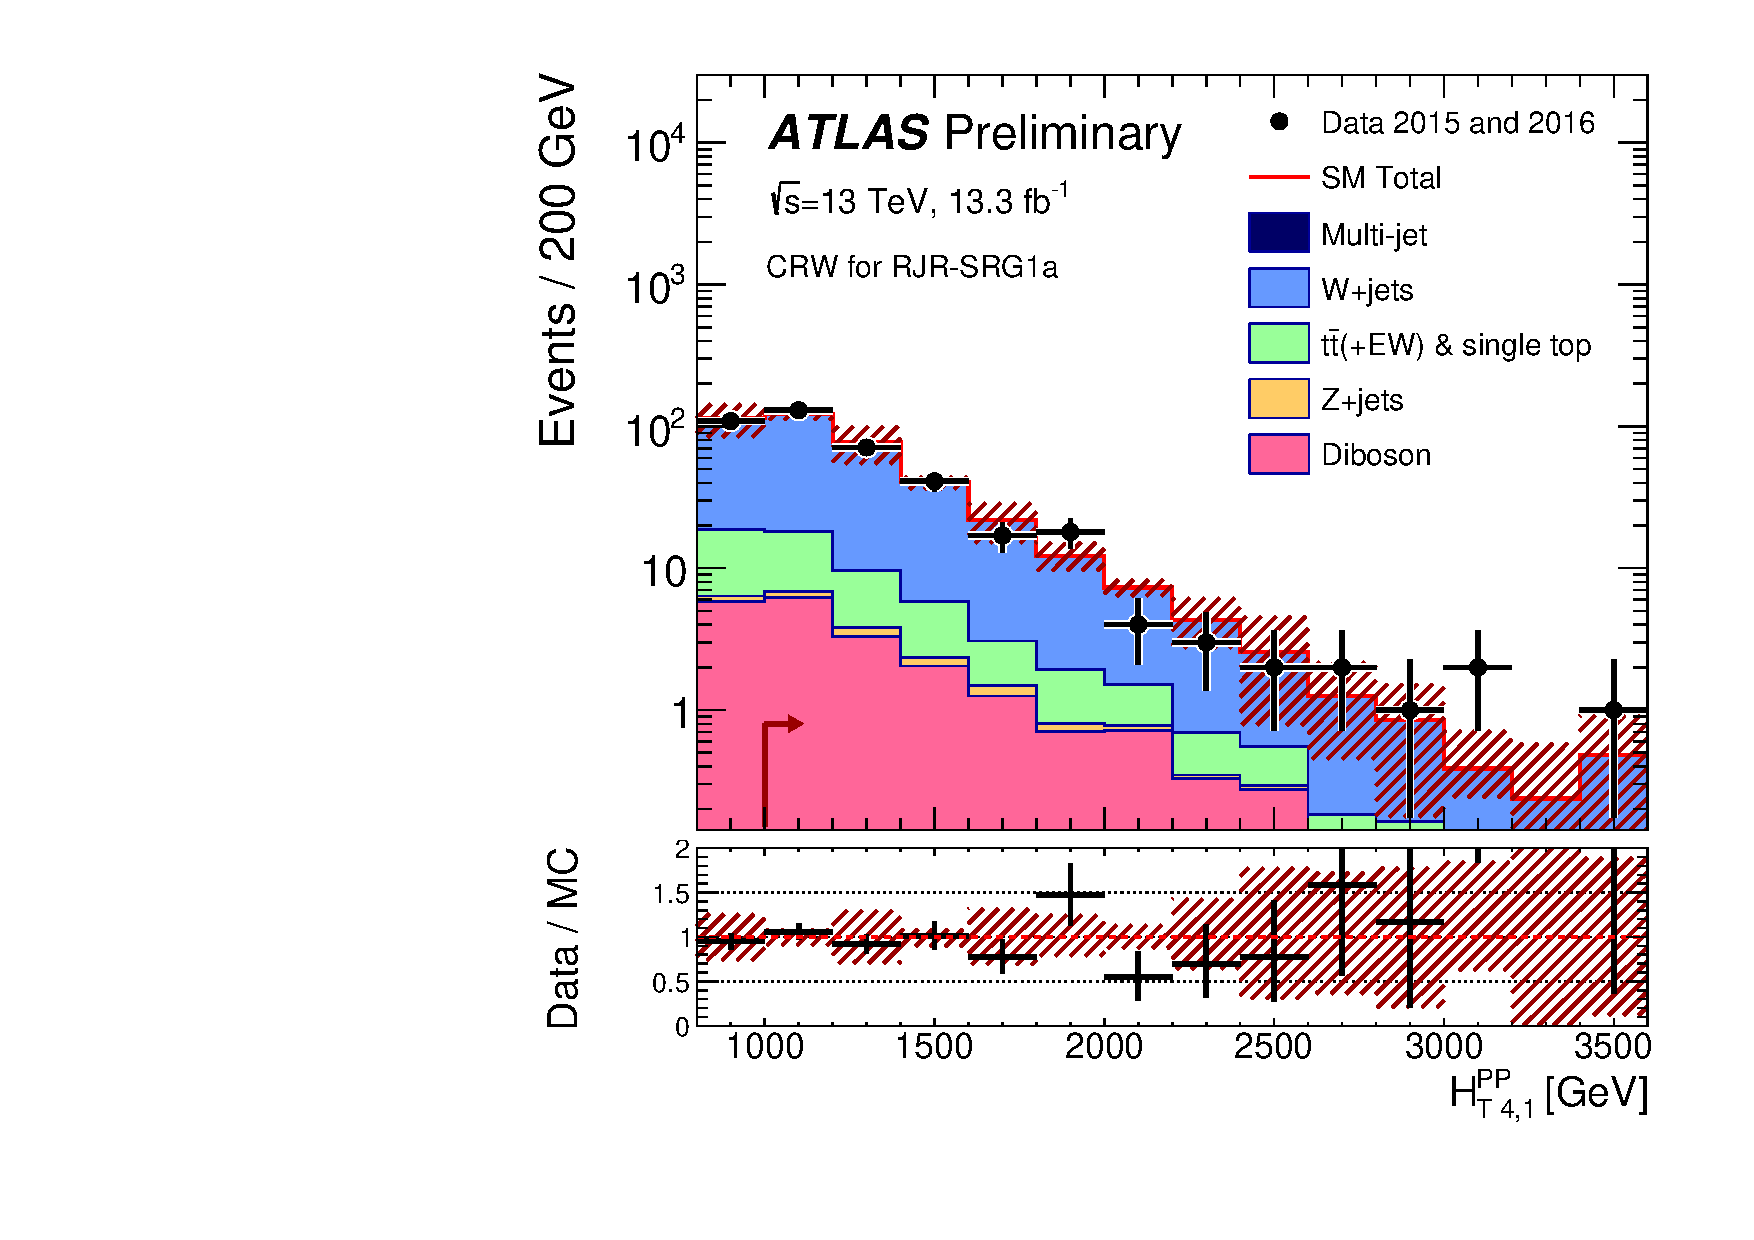
\includegraphics[width=0.45\textwidth]{figures/ATLAS-CONF-2016-078_INT/N-1Plots/AtlasStyle/Preliminary/CRW_SRJigsawSRG1a_LastCut_CRW_minusone}
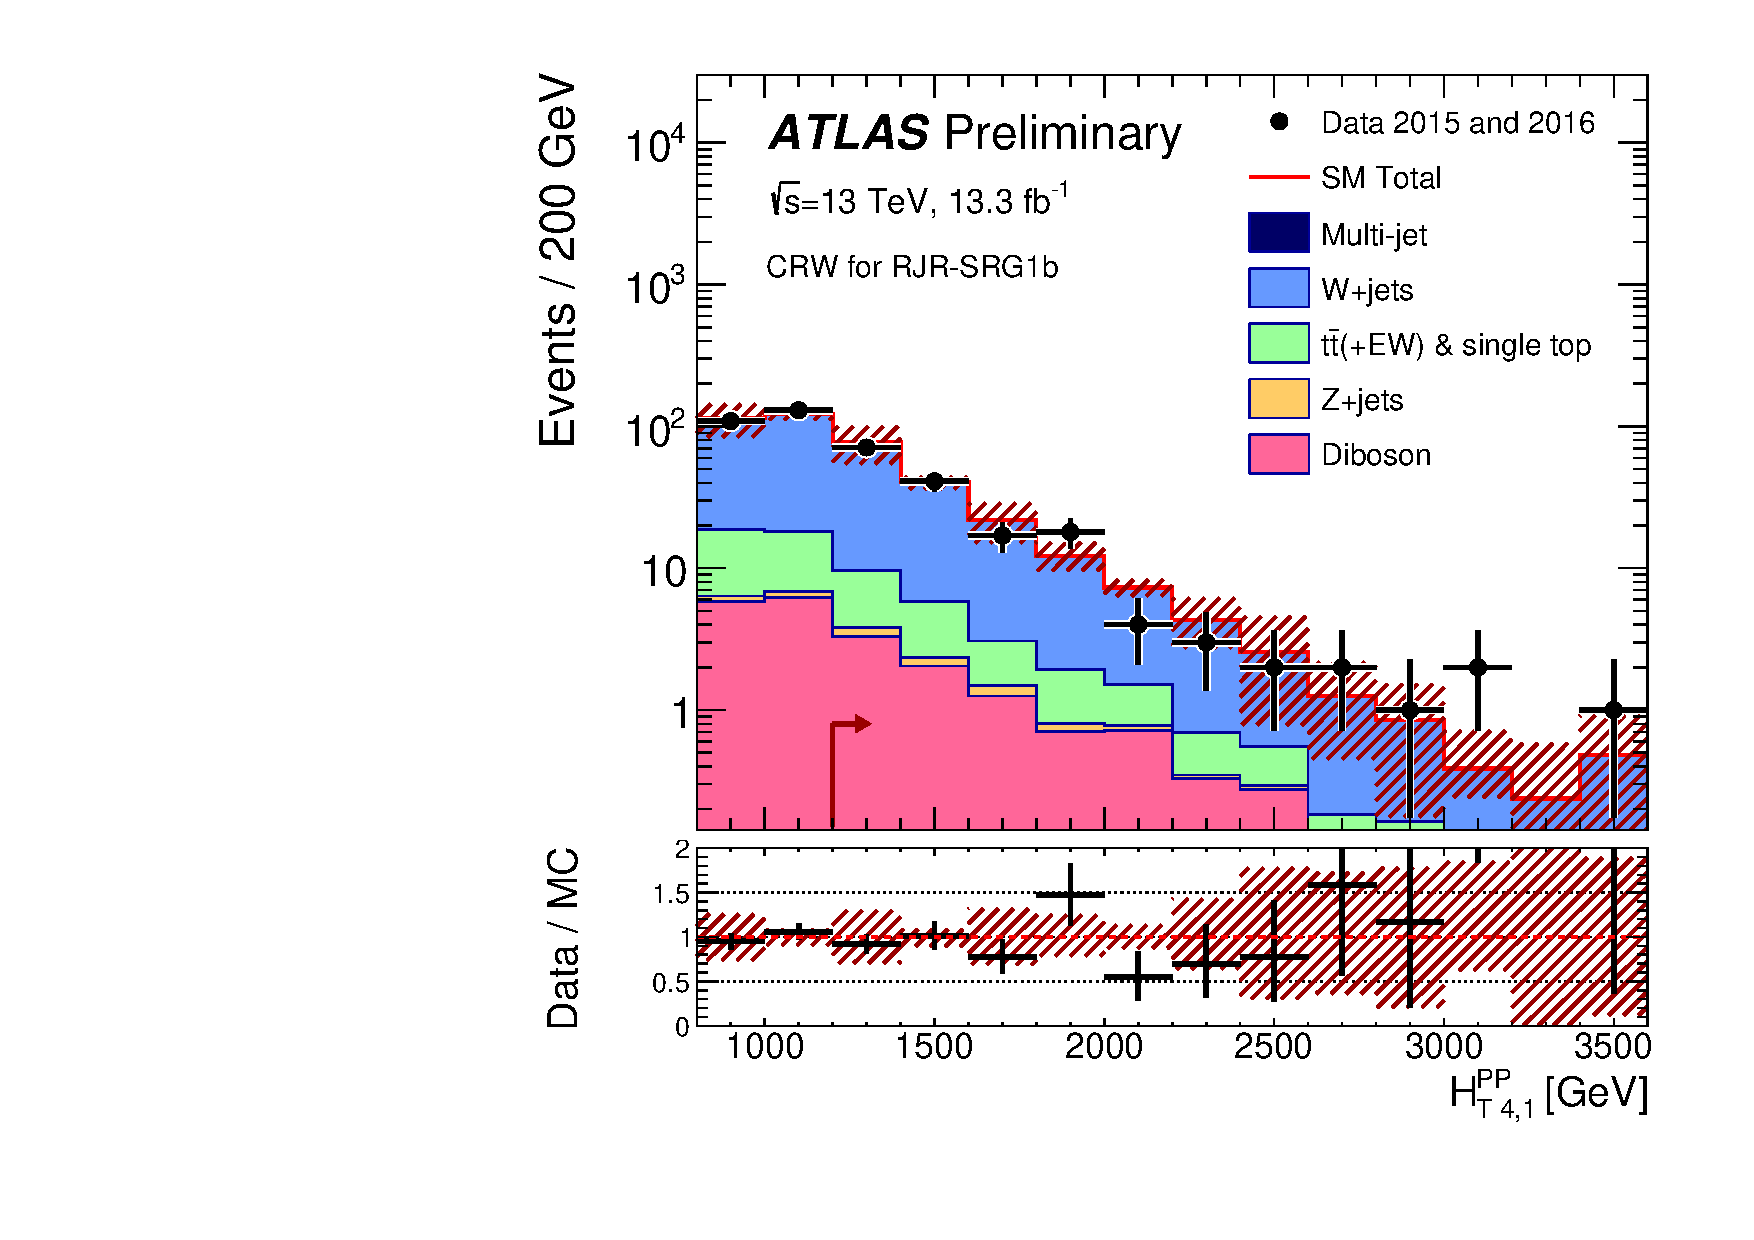
\includegraphics[width=0.45\textwidth]{figures/ATLAS-CONF-2016-078_INT/N-1Plots/AtlasStyle/Preliminary/CRW_SRJigsawSRG1b_LastCut_CRW_minusone}
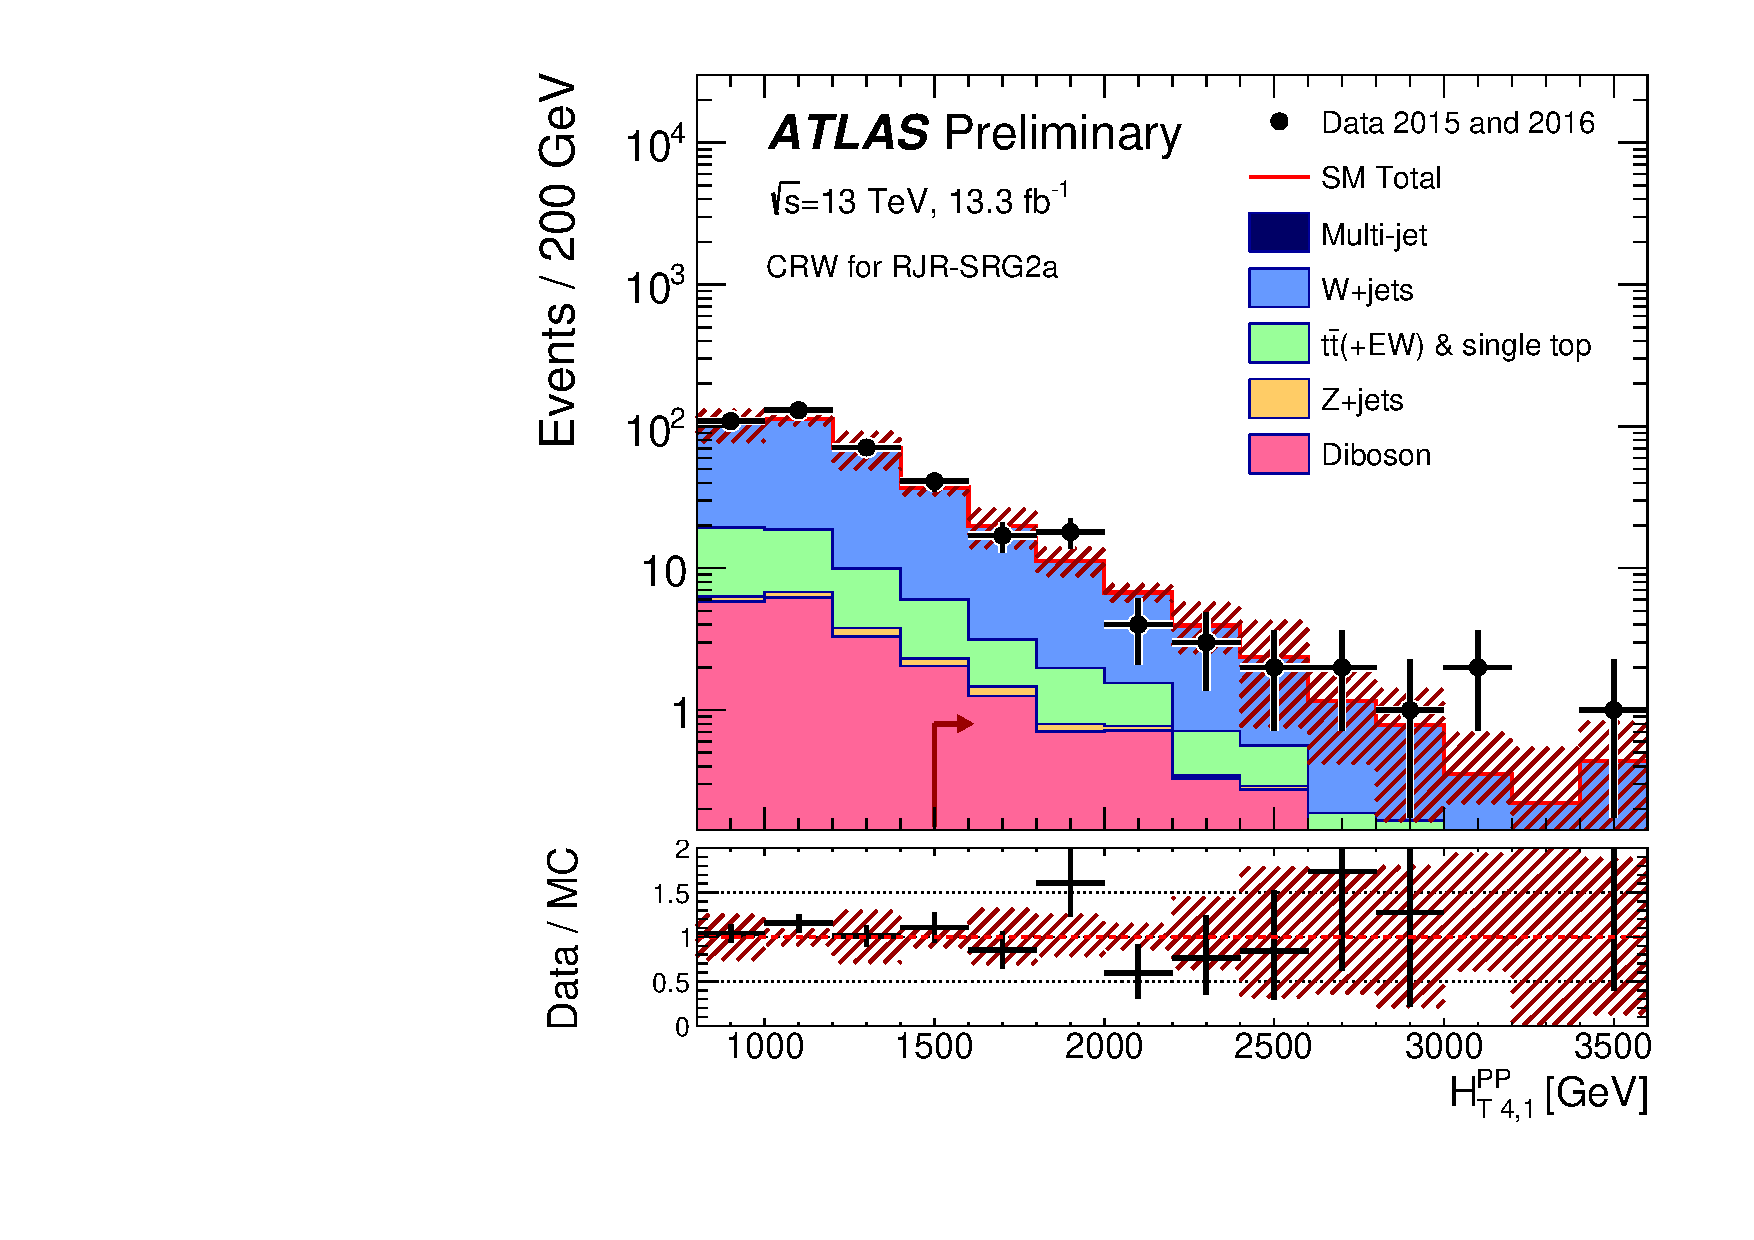
\includegraphics[width=0.45\textwidth]{figures/ATLAS-CONF-2016-078_INT/N-1Plots/AtlasStyle/Preliminary/CRW_SRJigsawSRG2a_LastCut_CRW_minusone}
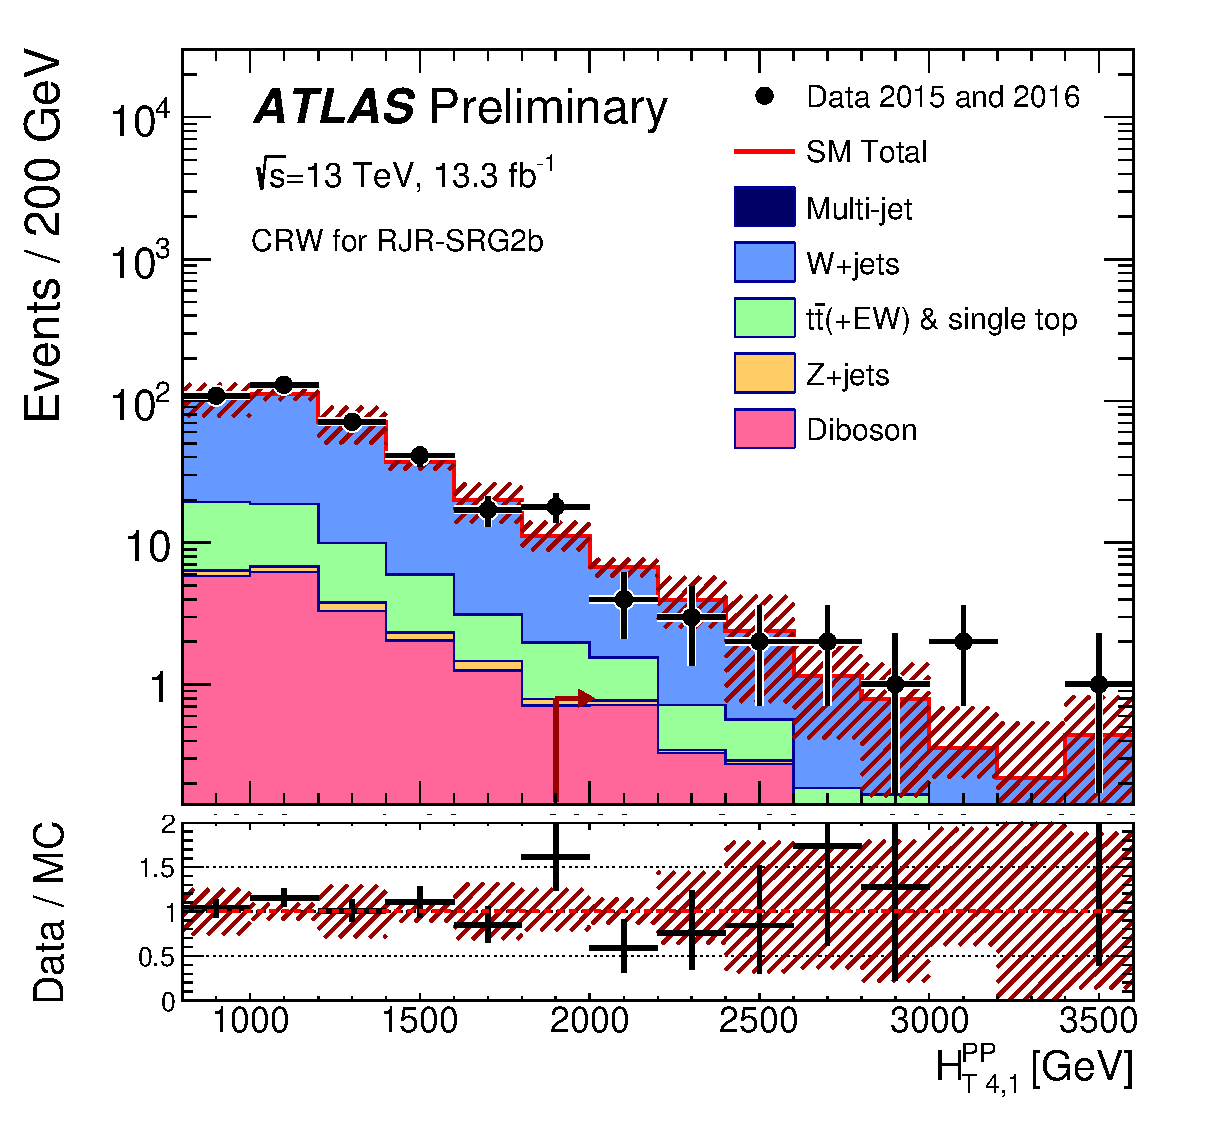
\includegraphics[width=0.45\textwidth]{figures/ATLAS-CONF-2016-078_INT/N-1Plots/AtlasStyle/Preliminary/CRW_SRJigsawSRG2b_LastCut_CRW_minusone}
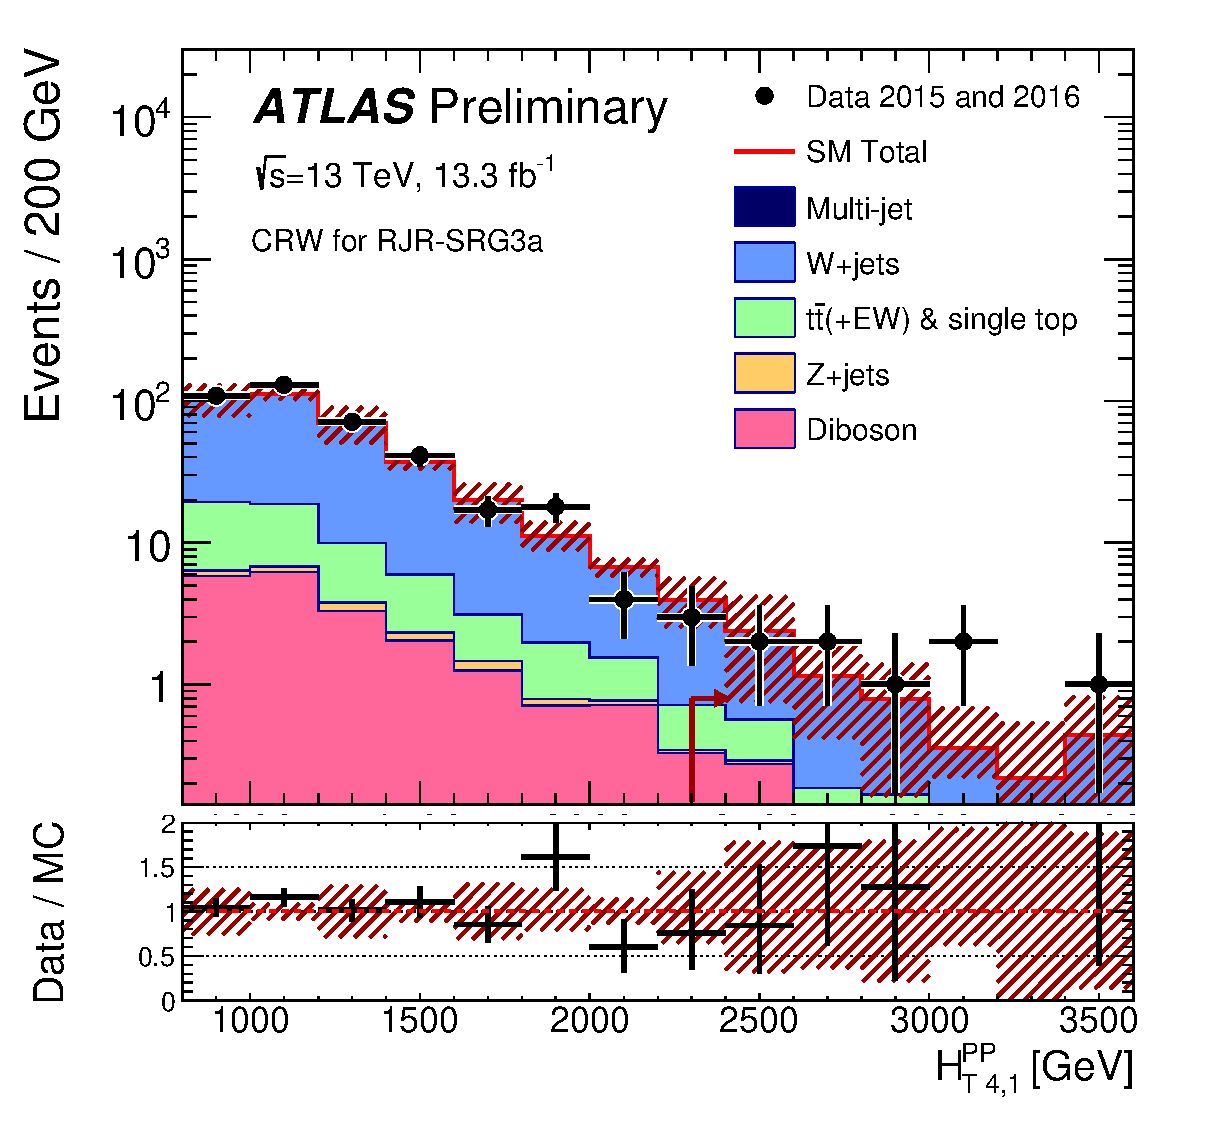
\includegraphics[width=0.45\textwidth]{figures/ATLAS-CONF-2016-078_INT/N-1Plots/AtlasStyle/Preliminary/CRW_SRJigsawSRG3a_LastCut_CRW_minusone}
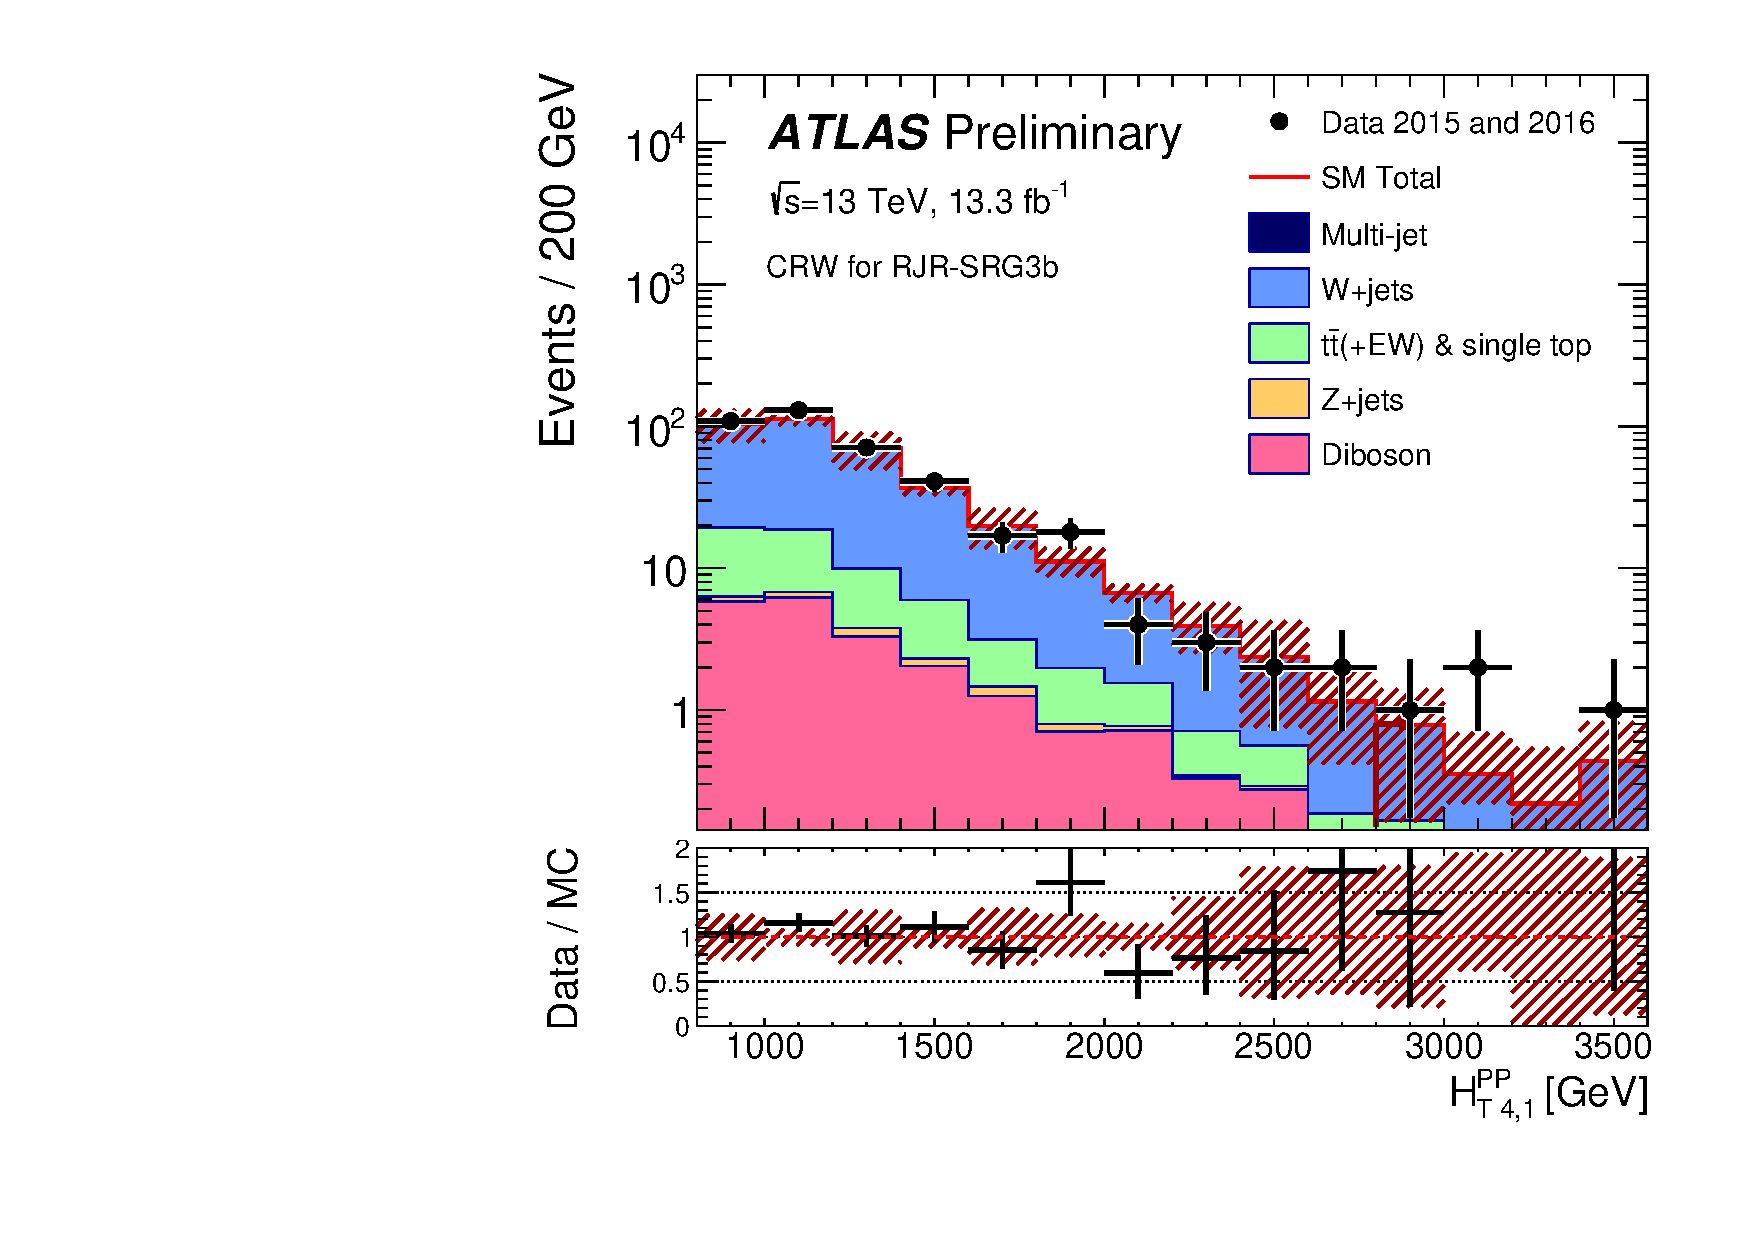
\includegraphics[width=0.45\textwidth]{figures/ATLAS-CONF-2016-078_INT/N-1Plots/AtlasStyle/Preliminary/CRW_SRJigsawSRG3b_LastCut_CRW_minusone}
\end{center}
\caption{Scale variable distributions for the gluino CRW regions.}
\label{fig:CRW_SRJigsawSRG1a_LastCut_CRW_minusone}
\end{figure}

\begin{figure}[tbph]
\begin{center}
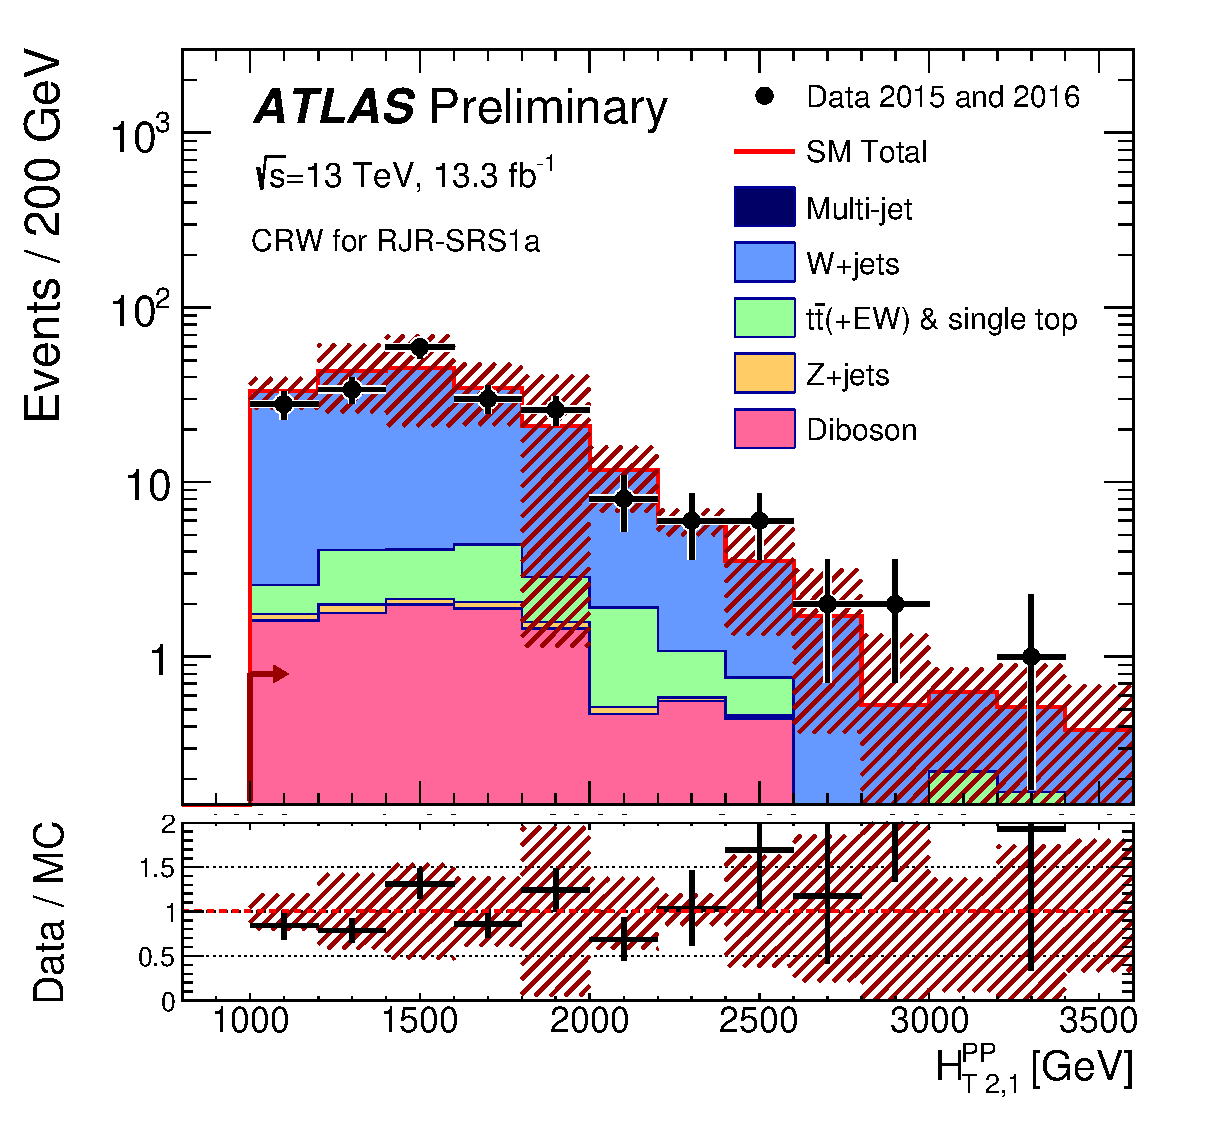
\includegraphics[width=0.45\textwidth]{figures/ATLAS-CONF-2016-078_INT/N-1Plots/AtlasStyle/Preliminary/CRW_SRJigsawSRS1a_LastCut_CRW_minusone}
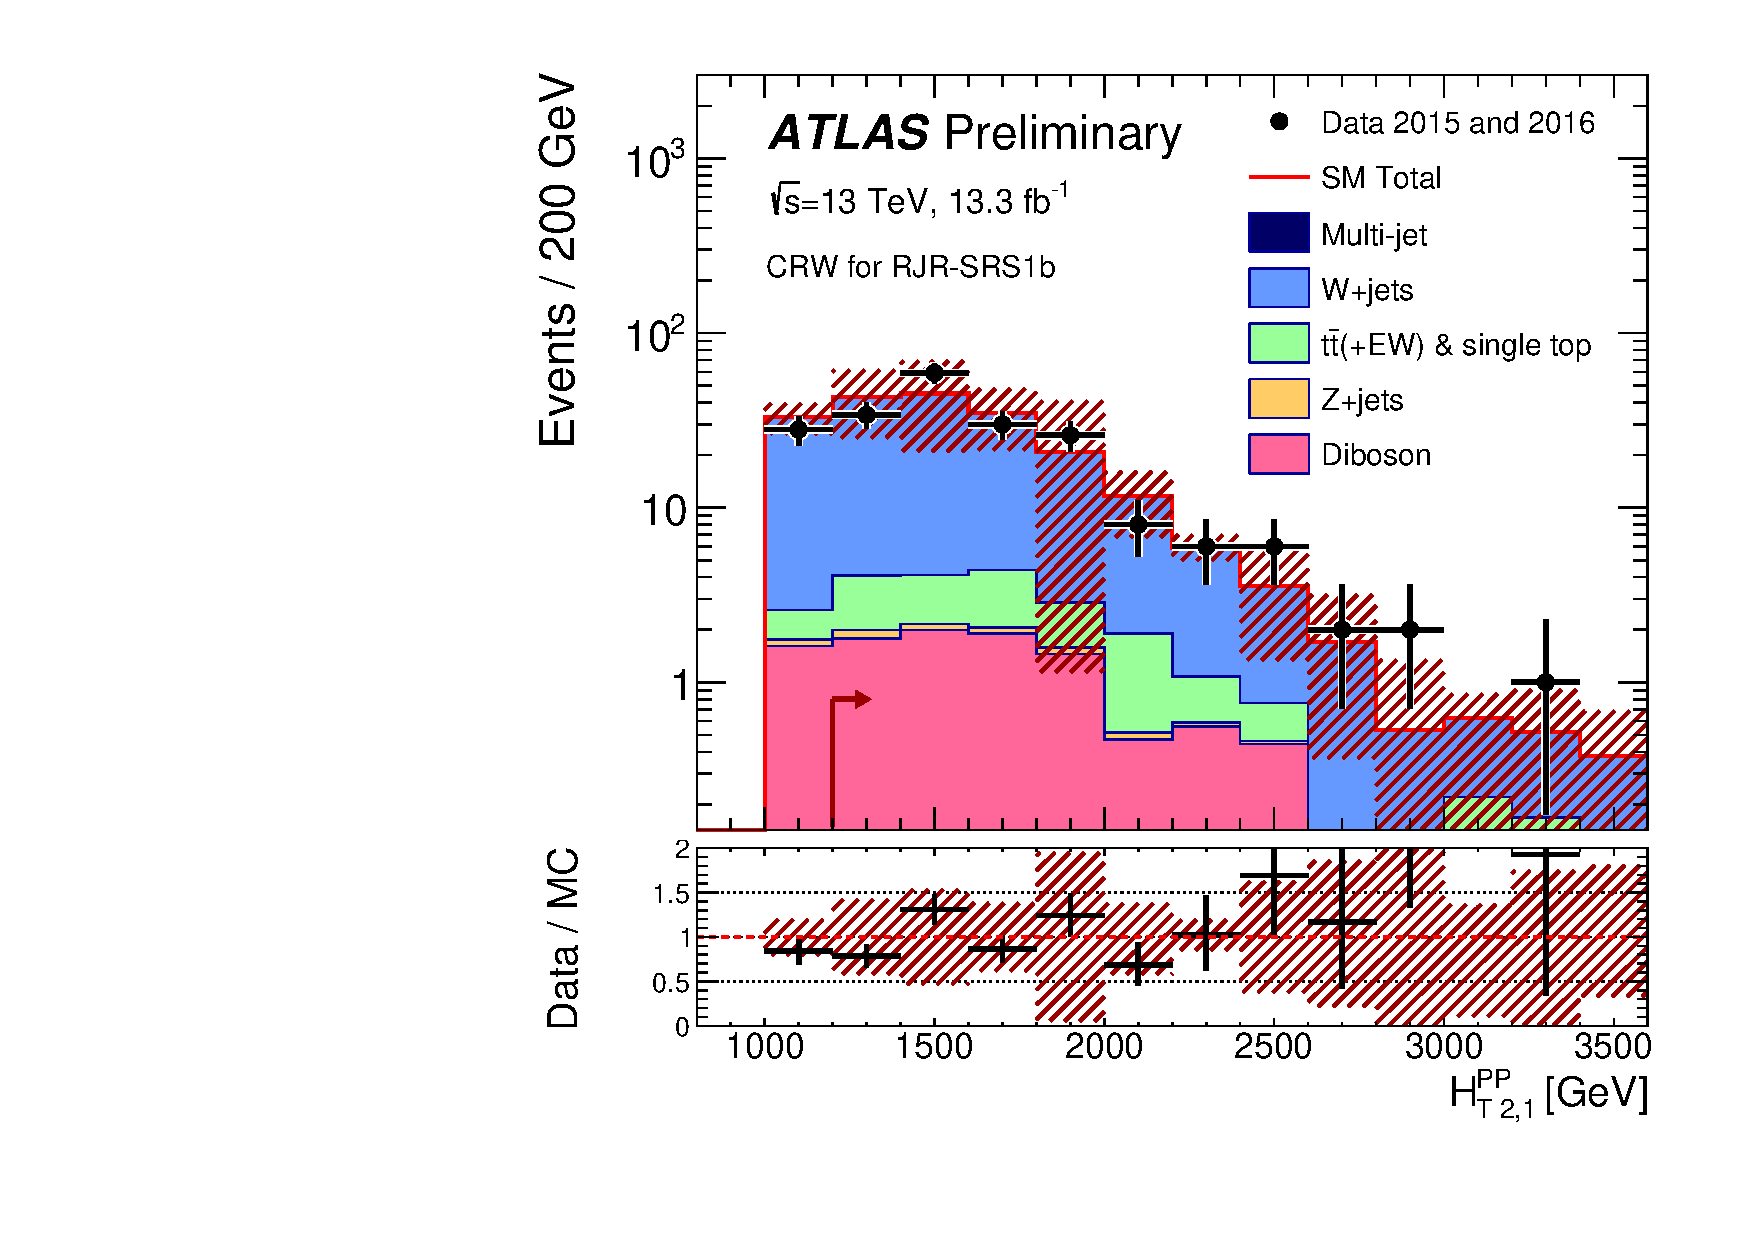
\includegraphics[width=0.45\textwidth]{figures/ATLAS-CONF-2016-078_INT/N-1Plots/AtlasStyle/Preliminary/CRW_SRJigsawSRS1b_LastCut_CRW_minusone}
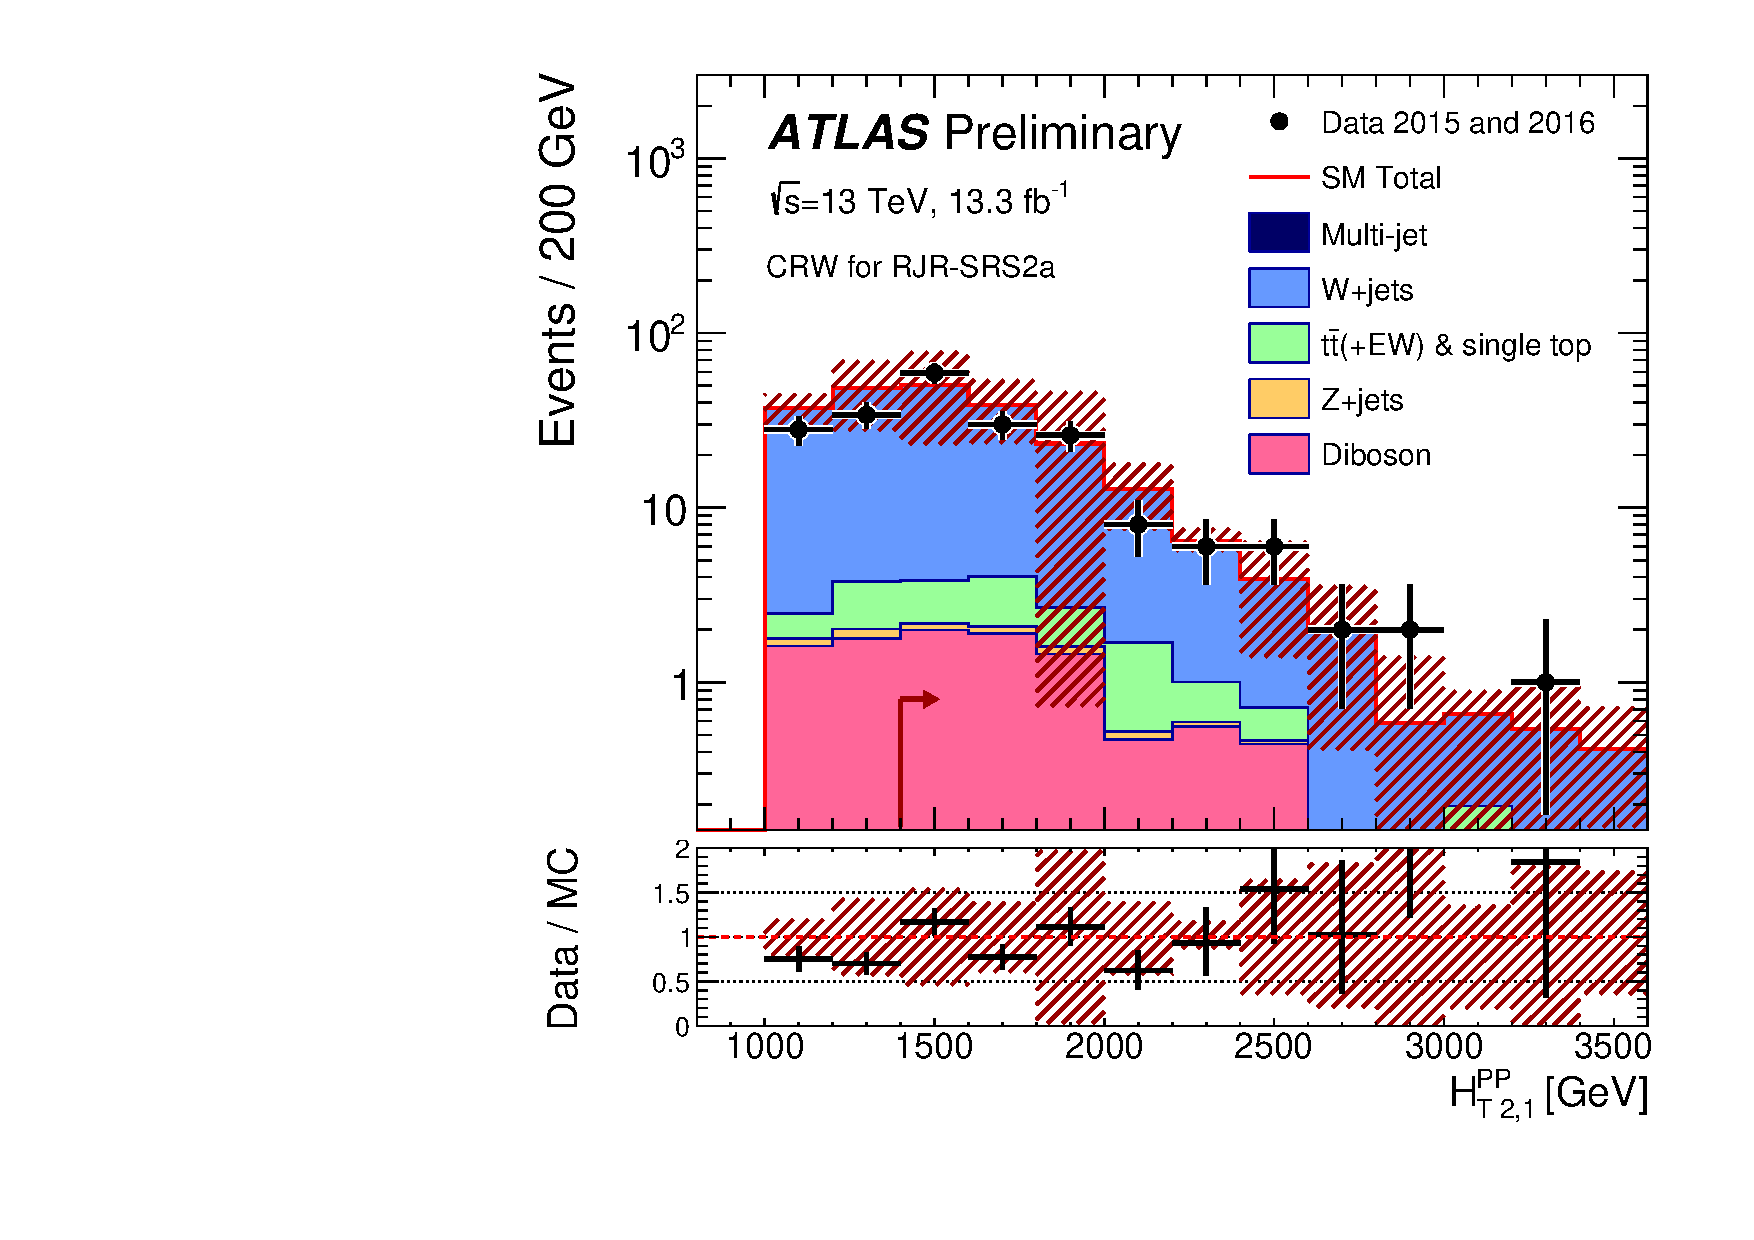
\includegraphics[width=0.45\textwidth]{figures/ATLAS-CONF-2016-078_INT/N-1Plots/AtlasStyle/Preliminary/CRW_SRJigsawSRS2a_LastCut_CRW_minusone}
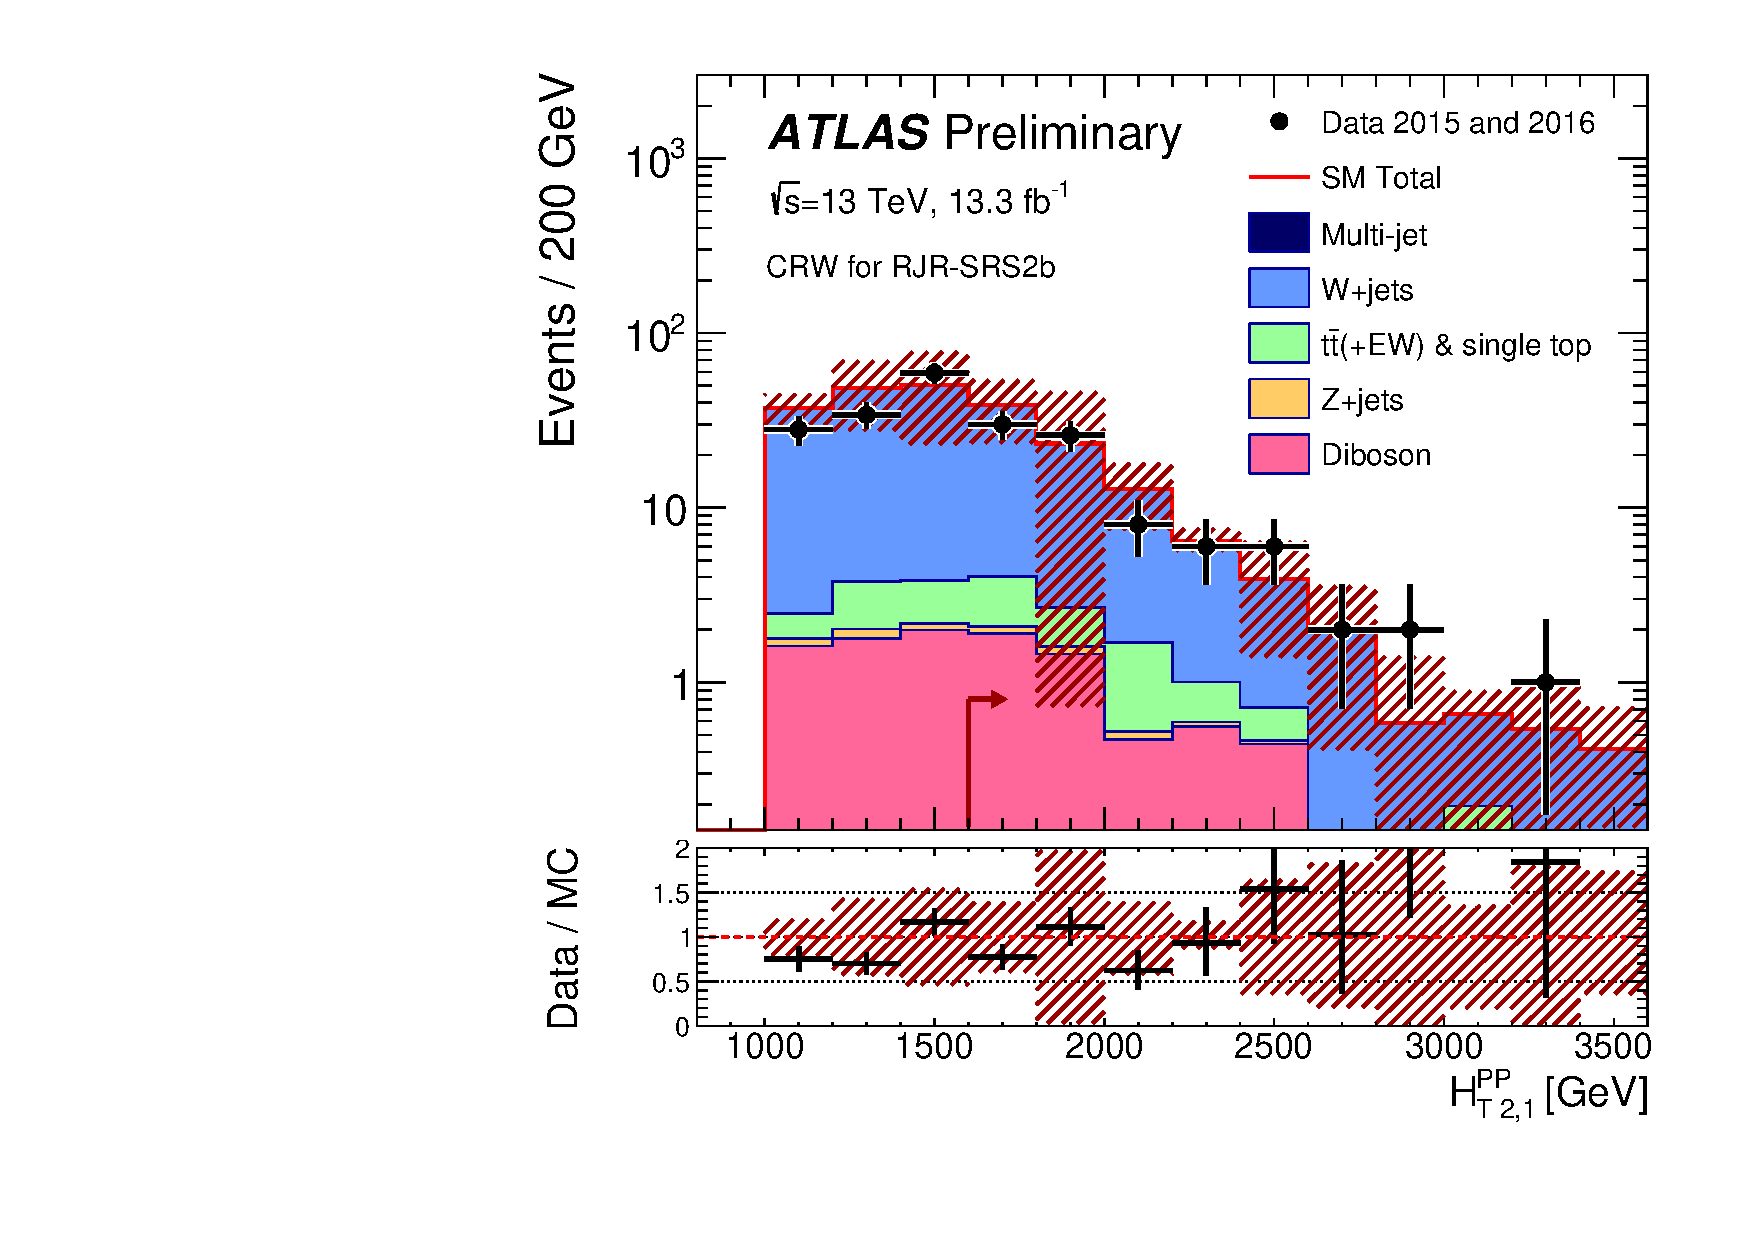
\includegraphics[width=0.45\textwidth]{figures/ATLAS-CONF-2016-078_INT/N-1Plots/AtlasStyle/Preliminary/CRW_SRJigsawSRS2b_LastCut_CRW_minusone}
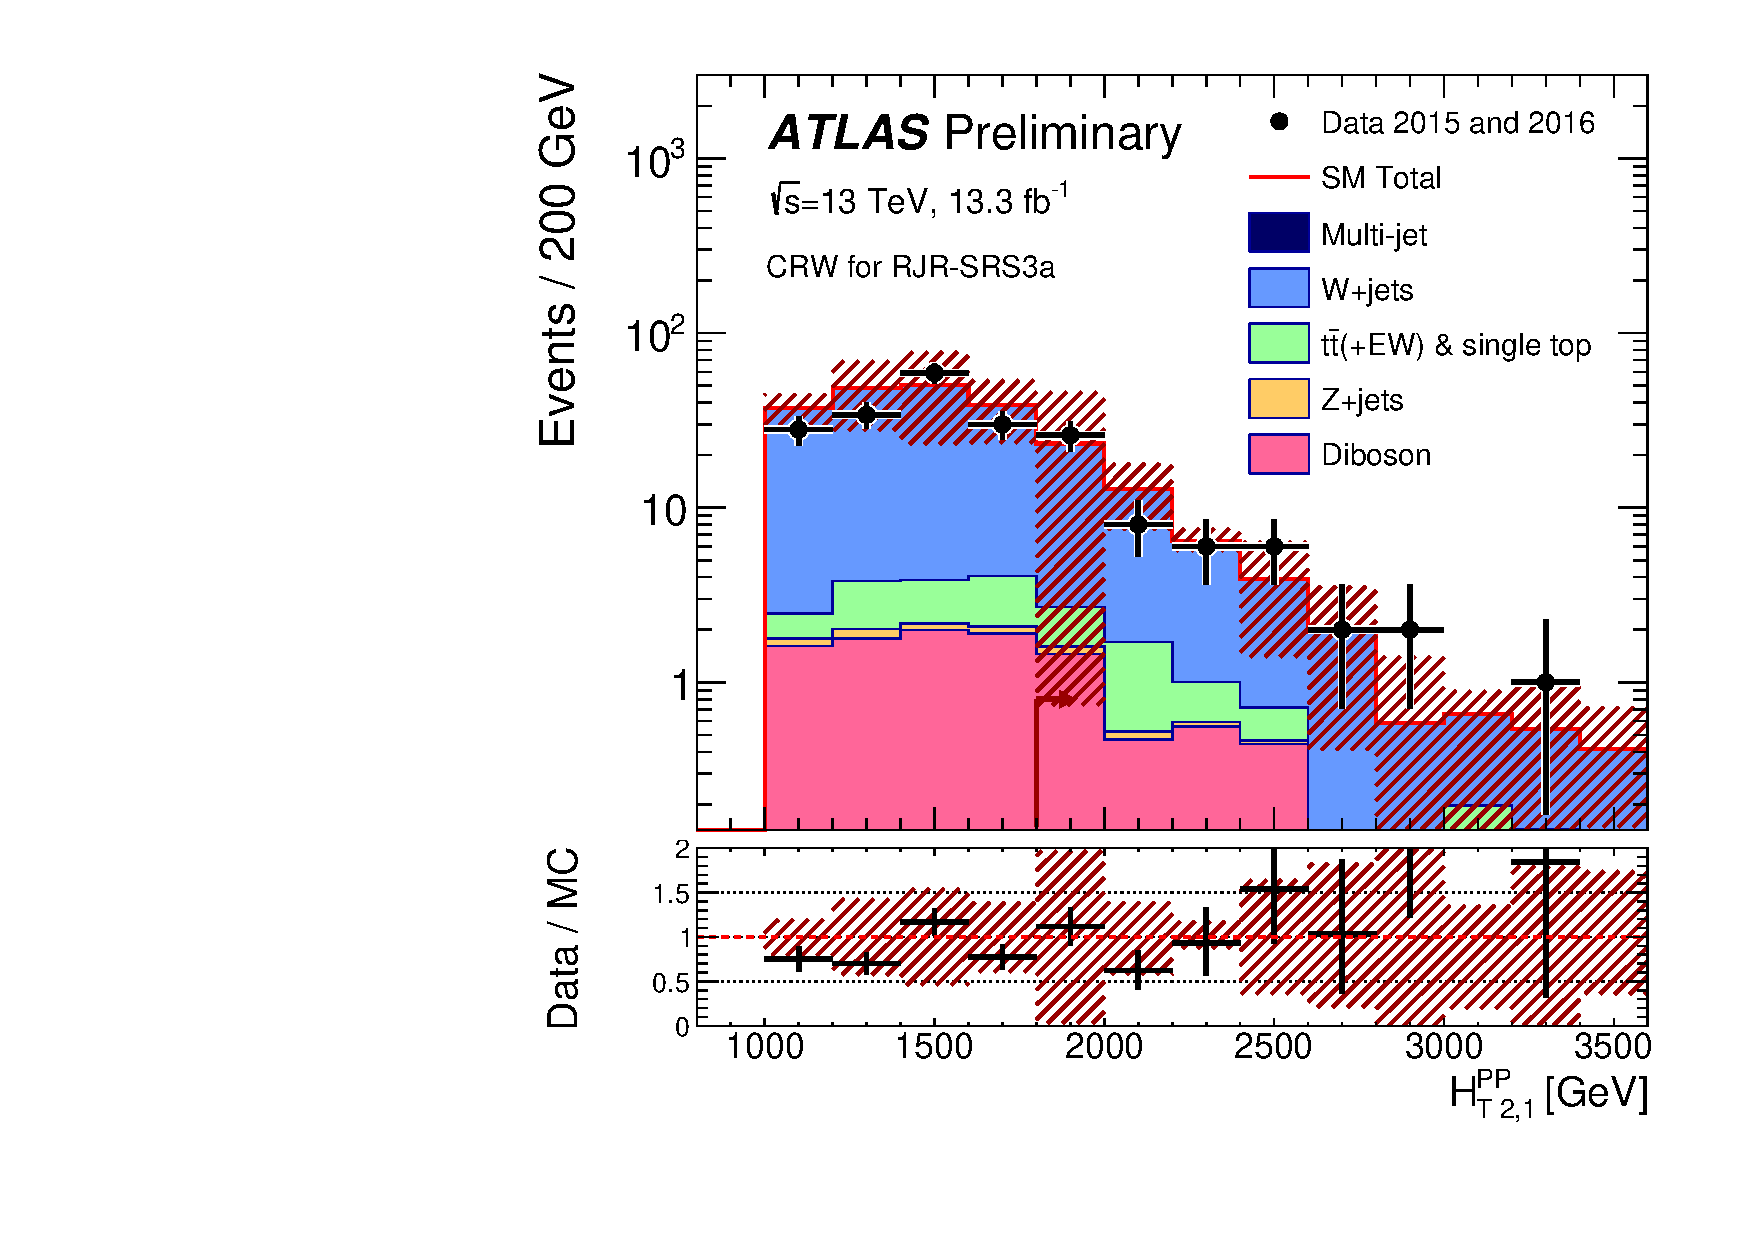
\includegraphics[width=0.45\textwidth]{figures/ATLAS-CONF-2016-078_INT/N-1Plots/AtlasStyle/Preliminary/CRW_SRJigsawSRS3a_LastCut_CRW_minusone}
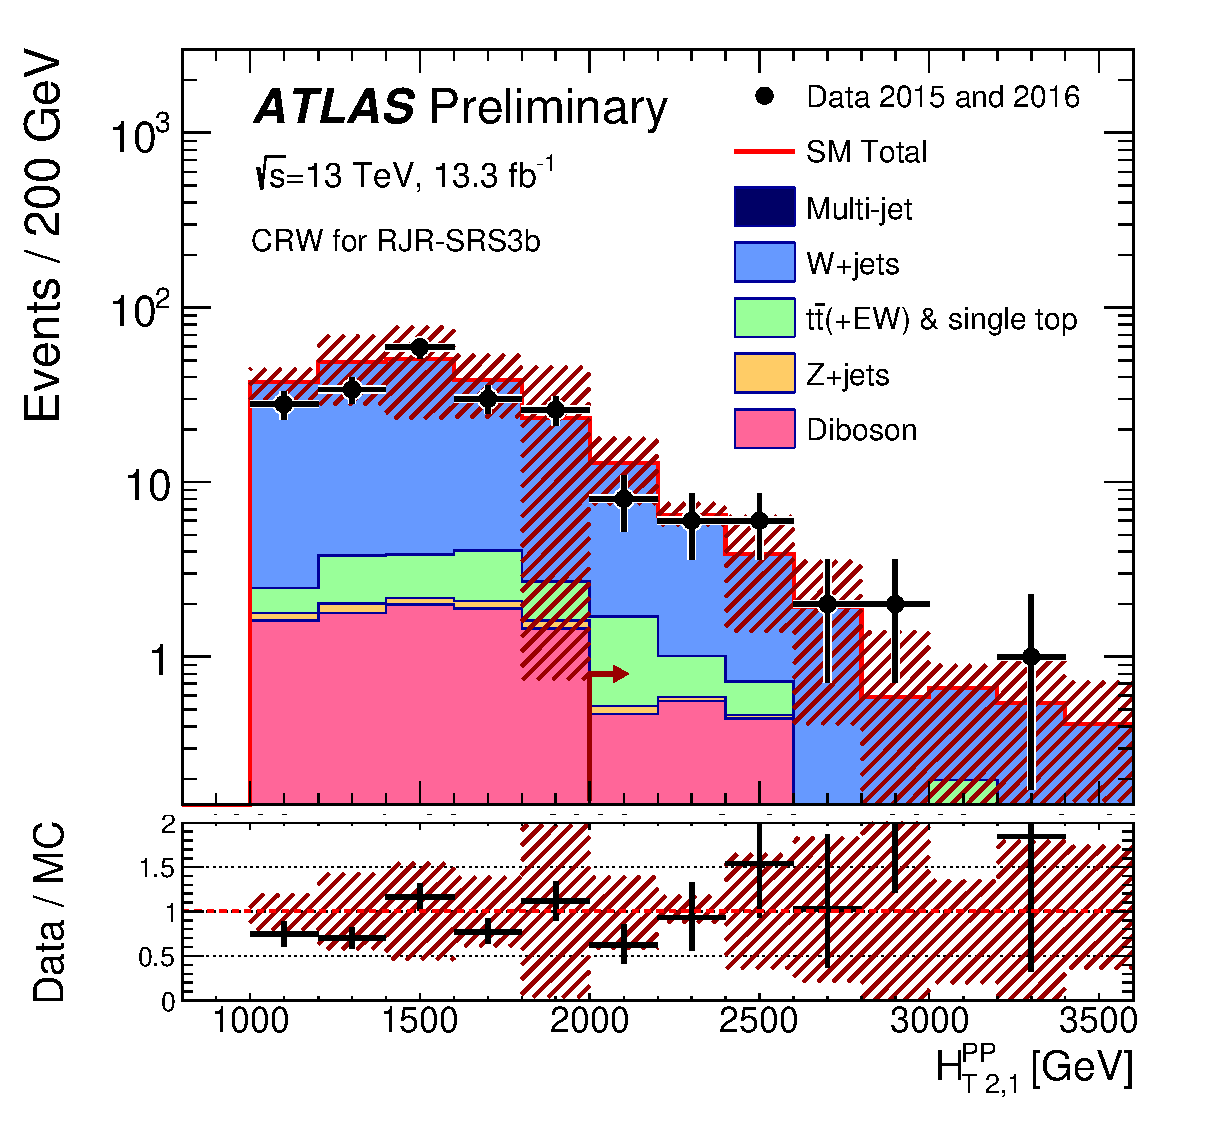
\includegraphics[width=0.45\textwidth]{figures/ATLAS-CONF-2016-078_INT/N-1Plots/AtlasStyle/Preliminary/CRW_SRJigsawSRS3b_LastCut_CRW_minusone}
\end{center}
\caption{Scale variable distributions for the squark CRW regions.}
\label{fig:CRW_SRJigsawSRS1a_LastCut_CRW_minusone}
\end{figure}


\clearpage

\begin{figure}[tbph]
\begin{center}
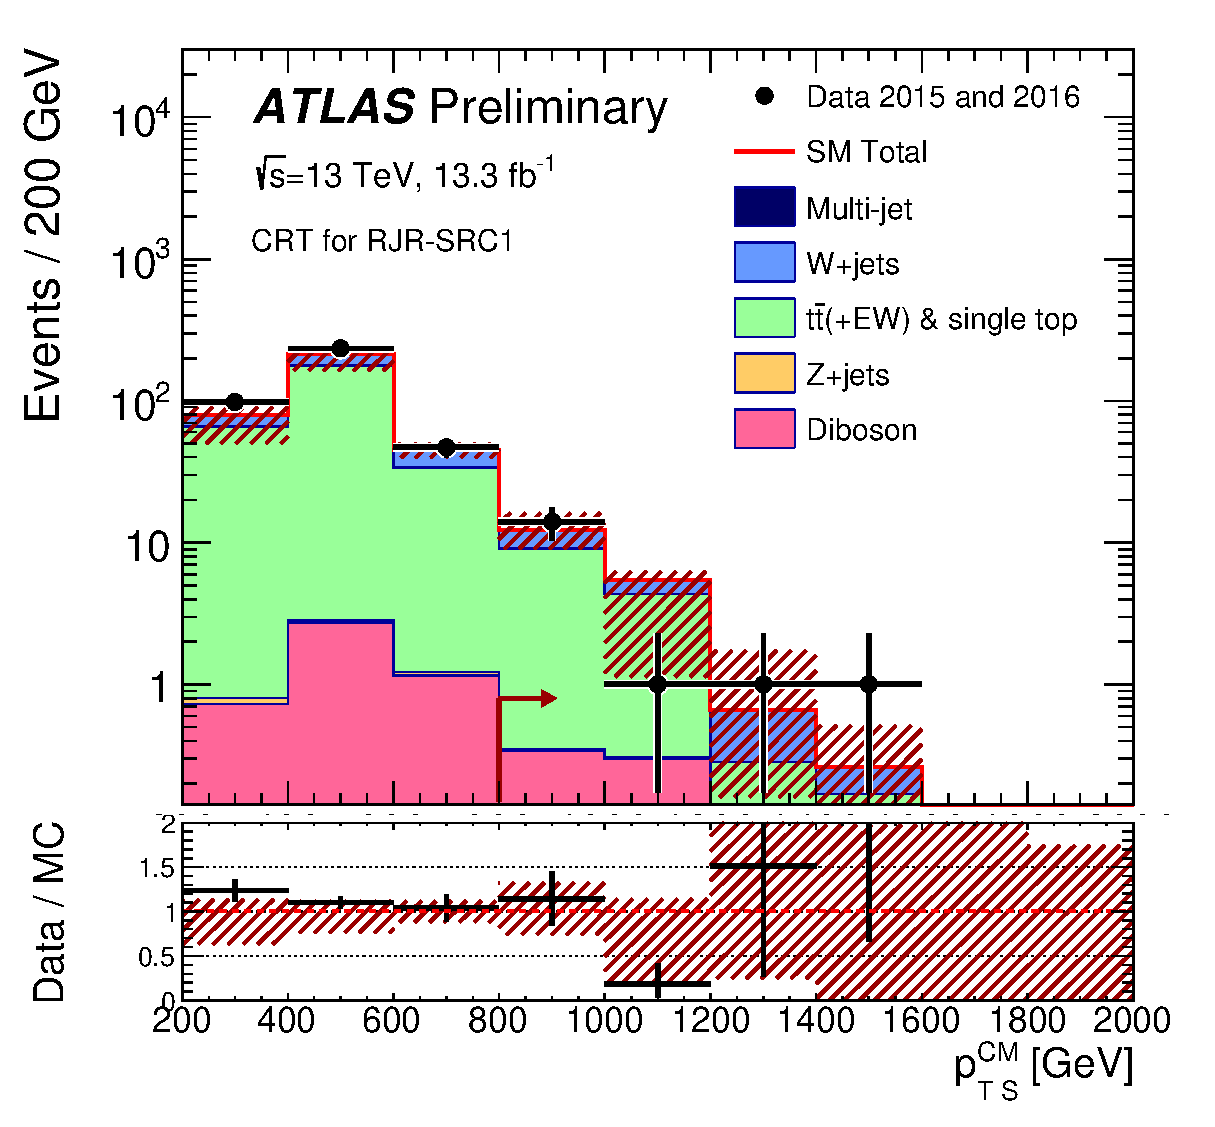
\includegraphics[width=0.45\textwidth]{figures/ATLAS-CONF-2016-078_INT/N-1Plots/AtlasStyle/Preliminary/CRT_SRJigsawSRC1_LastCut_CRT_minusone}
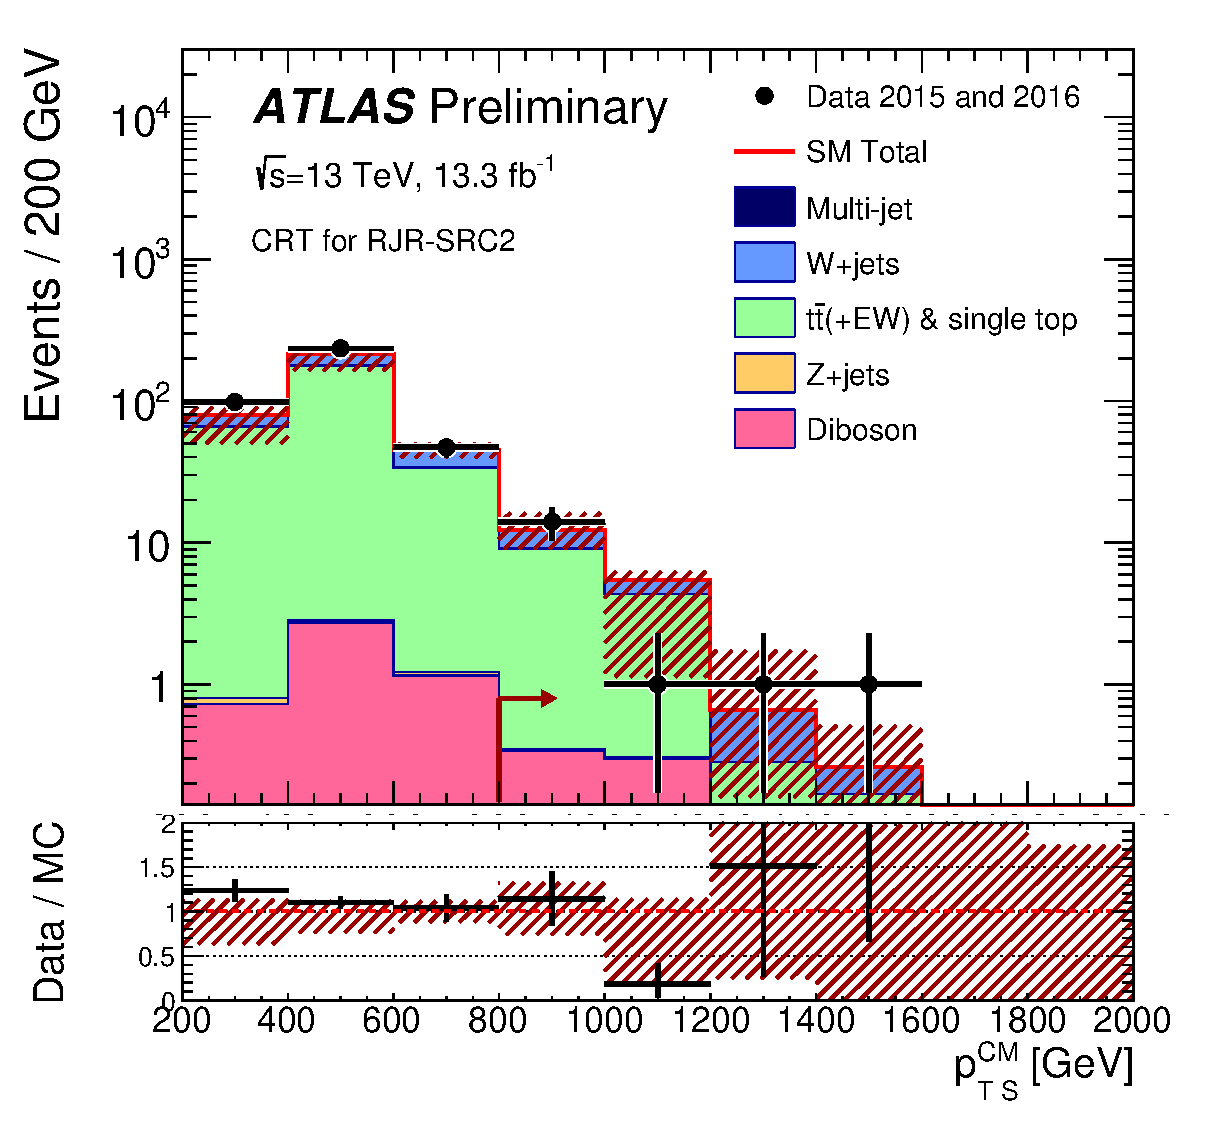
\includegraphics[width=0.45\textwidth]{figures/ATLAS-CONF-2016-078_INT/N-1Plots/AtlasStyle/Preliminary/CRT_SRJigsawSRC2_LastCut_CRT_minusone}
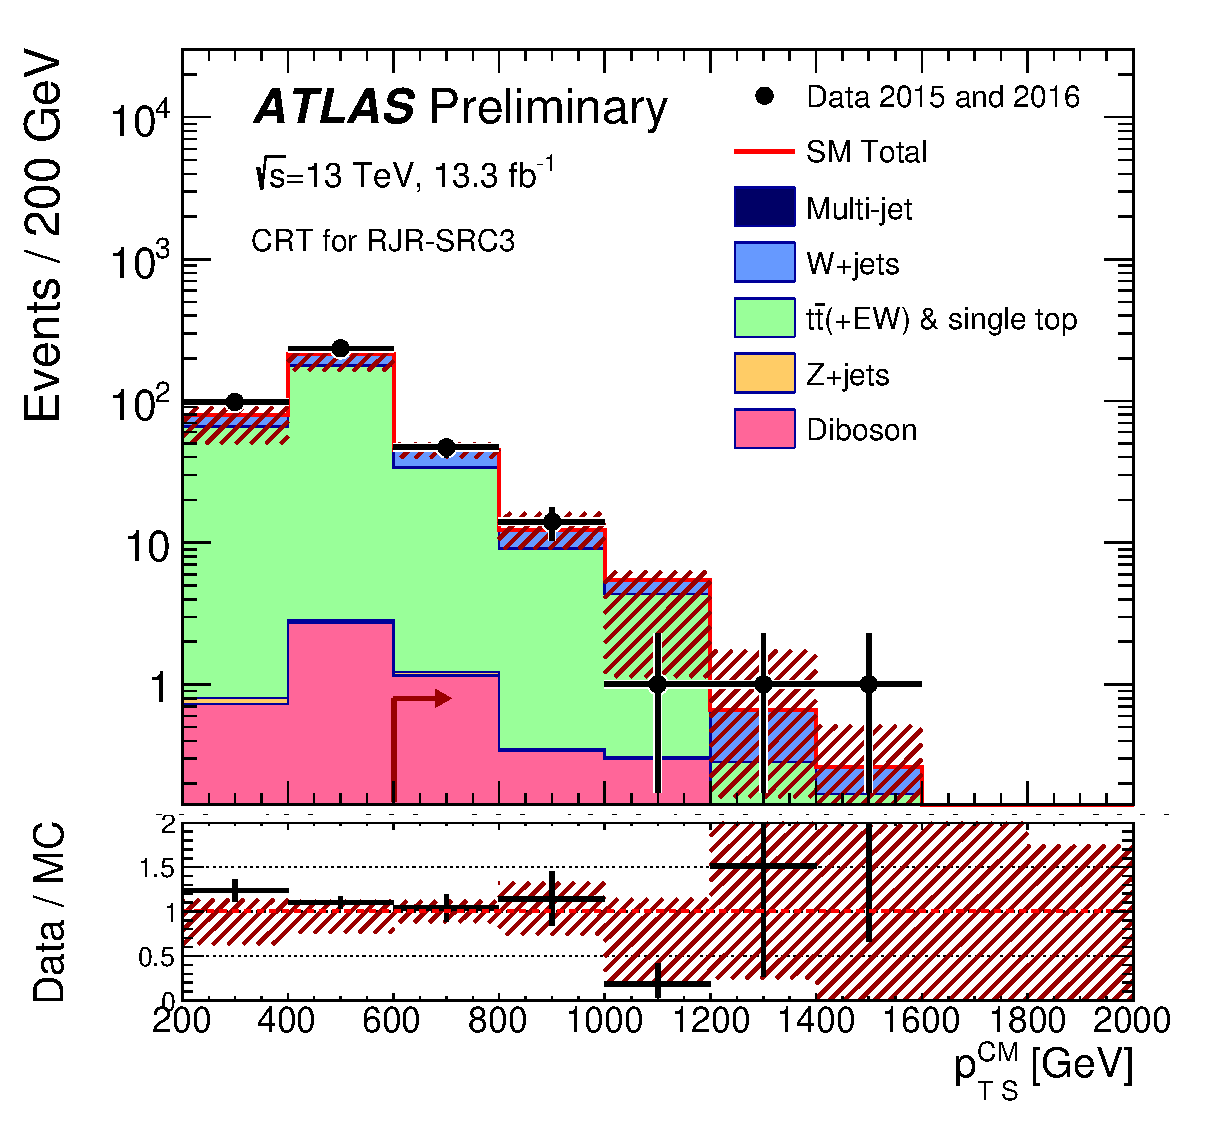
\includegraphics[width=0.45\textwidth]{figures/ATLAS-CONF-2016-078_INT/N-1Plots/AtlasStyle/Preliminary/CRT_SRJigsawSRC3_LastCut_CRT_minusone}
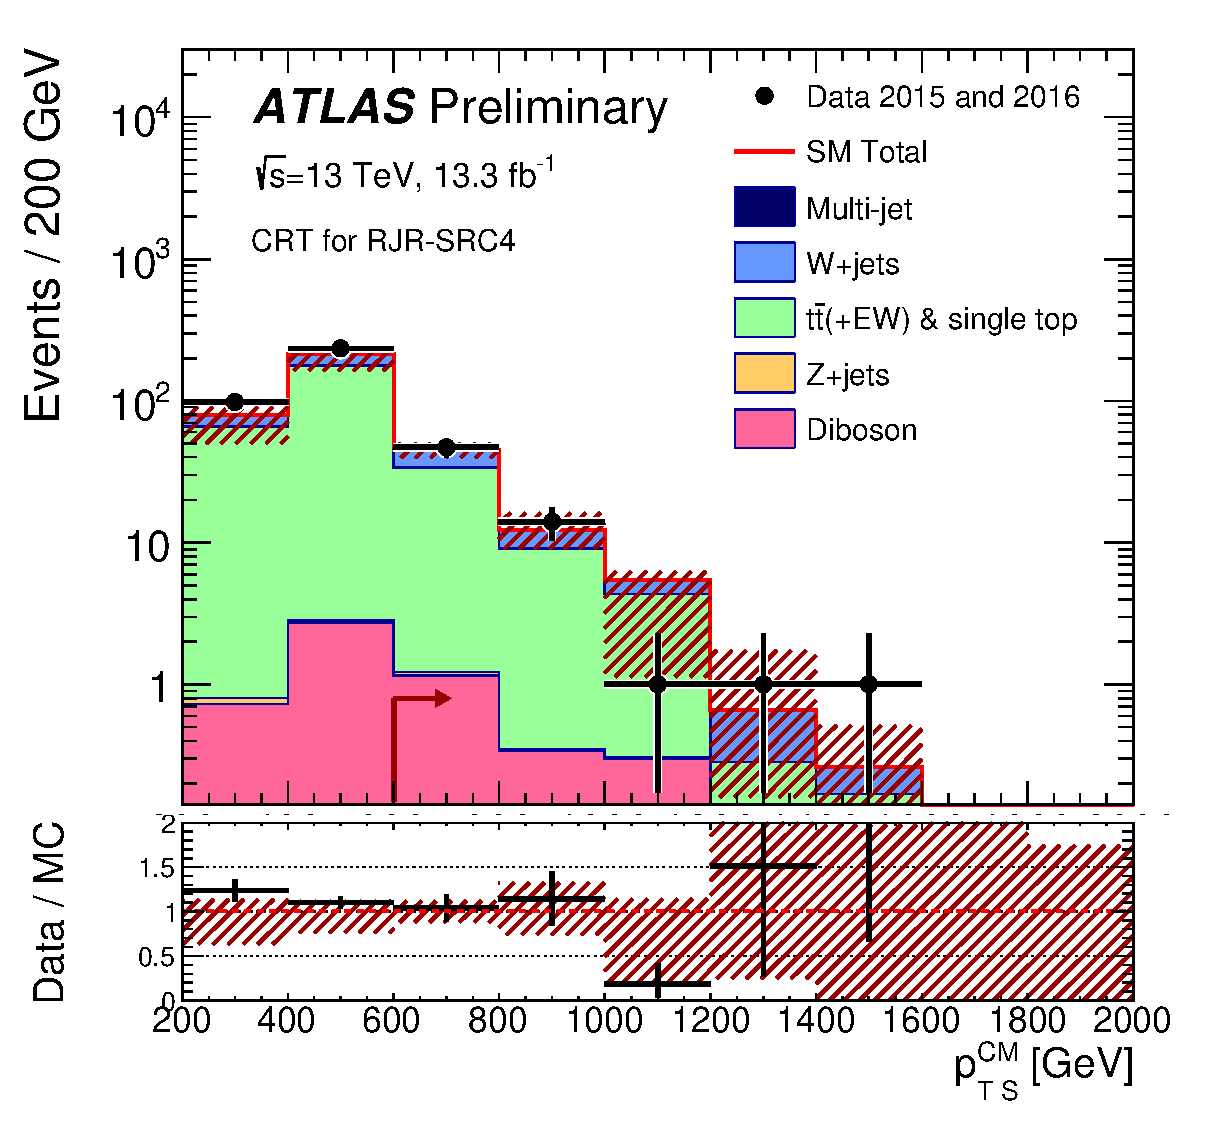
\includegraphics[width=0.45\textwidth]{figures/ATLAS-CONF-2016-078_INT/N-1Plots/AtlasStyle/Preliminary/CRT_SRJigsawSRC4_LastCut_CRT_minusone}
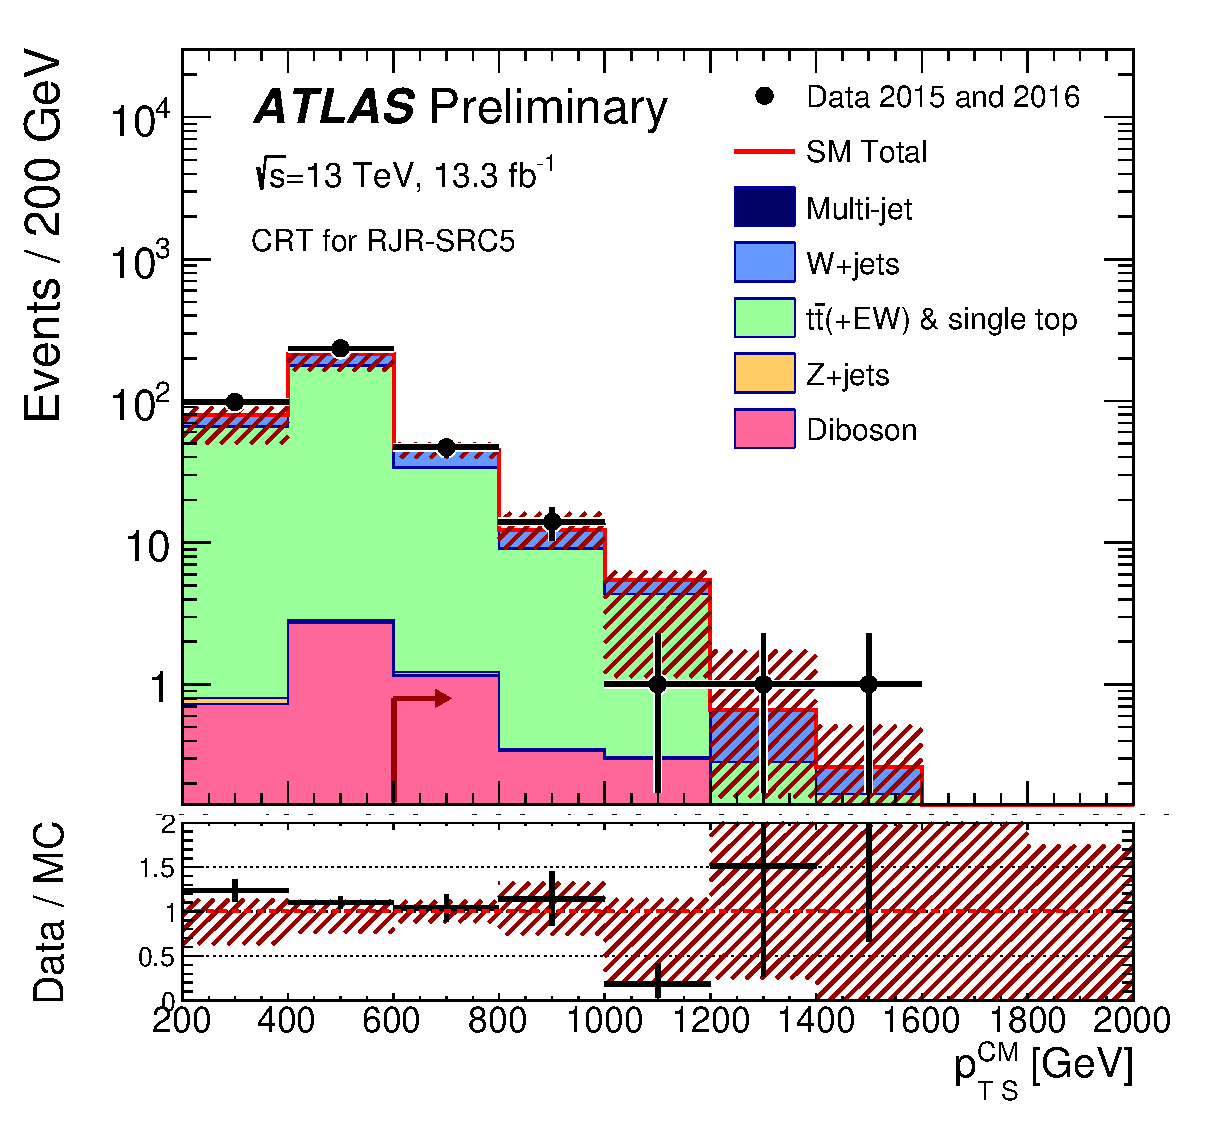
\includegraphics[width=0.45\textwidth]{figures/ATLAS-CONF-2016-078_INT/N-1Plots/AtlasStyle/Preliminary/CRT_SRJigsawSRC5_LastCut_CRT_minusone}
\end{center}
\caption{Scale variable distributions for the compressed CRT regions.}
\label{fig:CRT_SRJigsawSRC1_LastCut_CRT_minusone}
\end{figure}

\begin{figure}[tbph]
\begin{center}
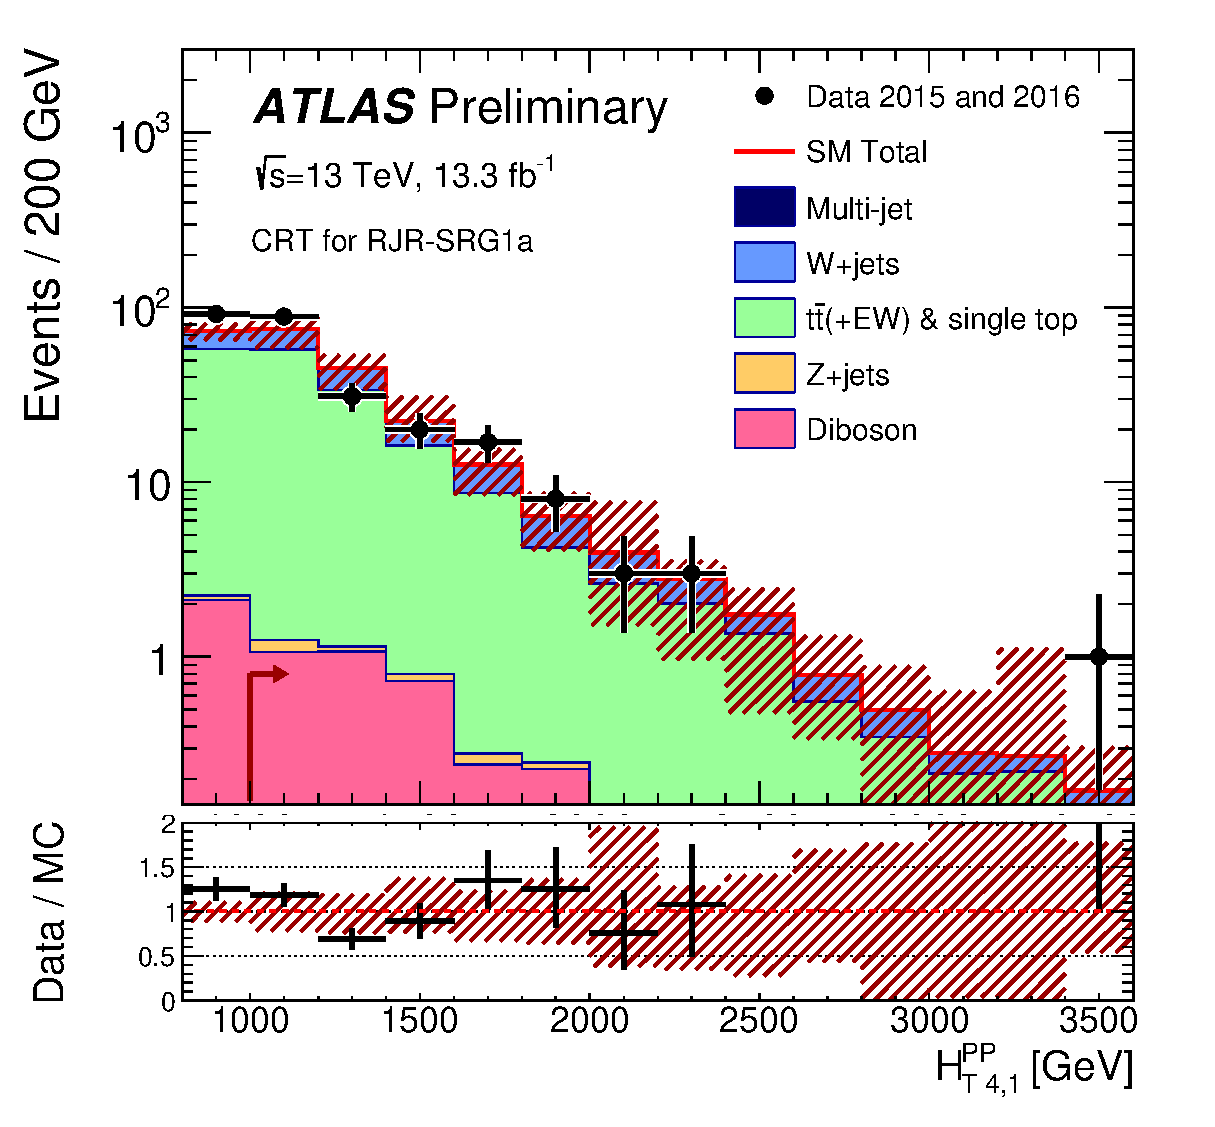
\includegraphics[width=0.45\textwidth]{figures/ATLAS-CONF-2016-078_INT/N-1Plots/AtlasStyle/Preliminary/CRT_SRJigsawSRG1a_LastCut_CRT_minusone}
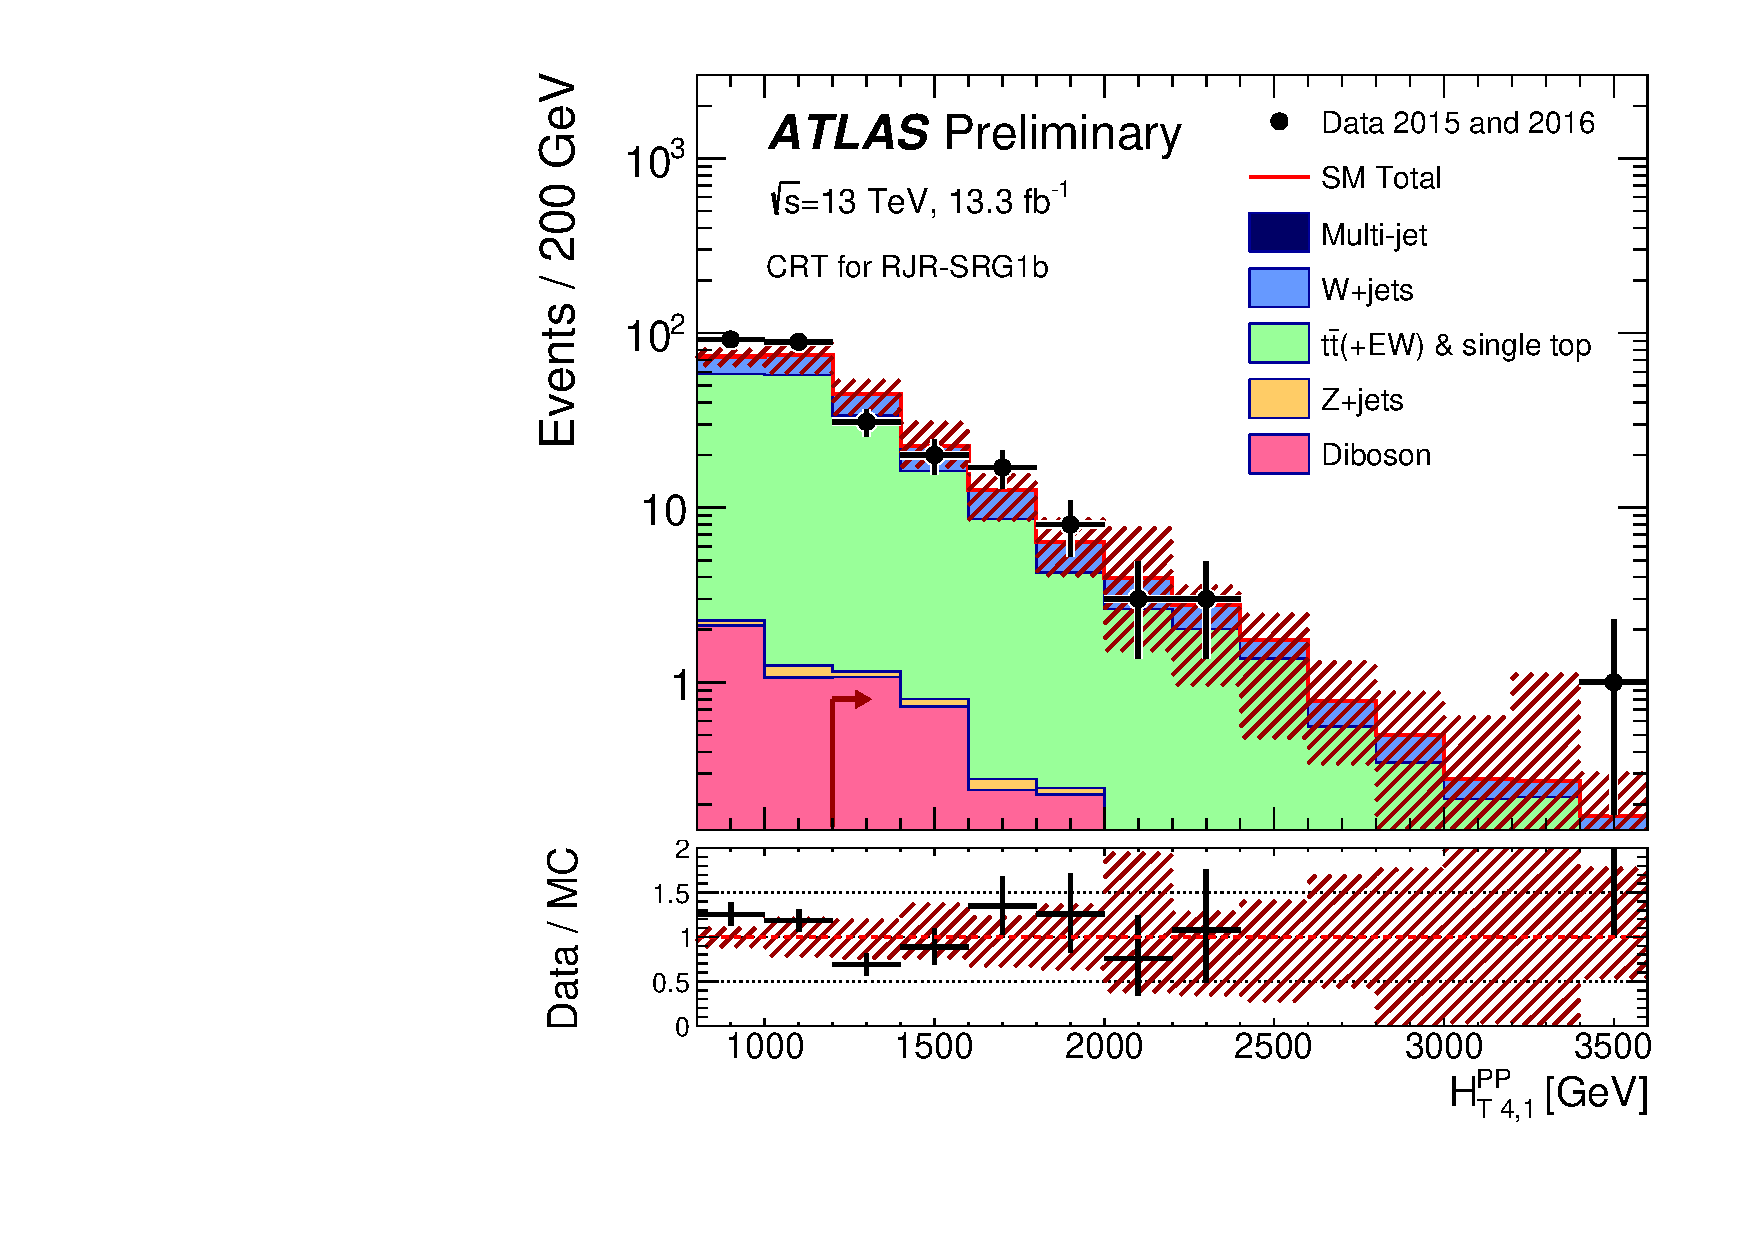
\includegraphics[width=0.45\textwidth]{figures/ATLAS-CONF-2016-078_INT/N-1Plots/AtlasStyle/Preliminary/CRT_SRJigsawSRG1b_LastCut_CRT_minusone}
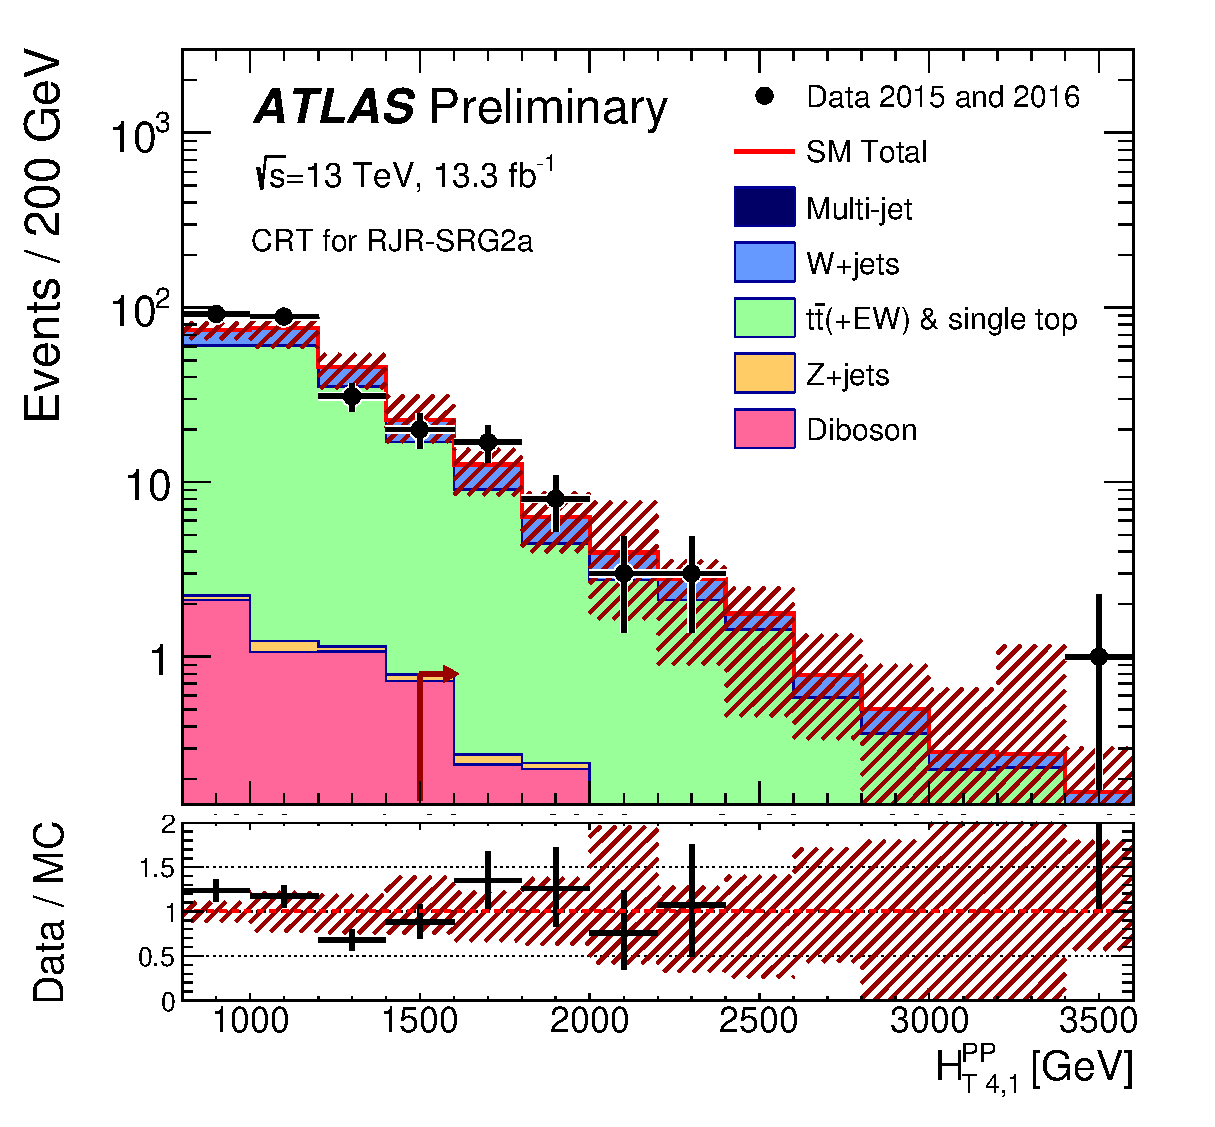
\includegraphics[width=0.45\textwidth]{figures/ATLAS-CONF-2016-078_INT/N-1Plots/AtlasStyle/Preliminary/CRT_SRJigsawSRG2a_LastCut_CRT_minusone}
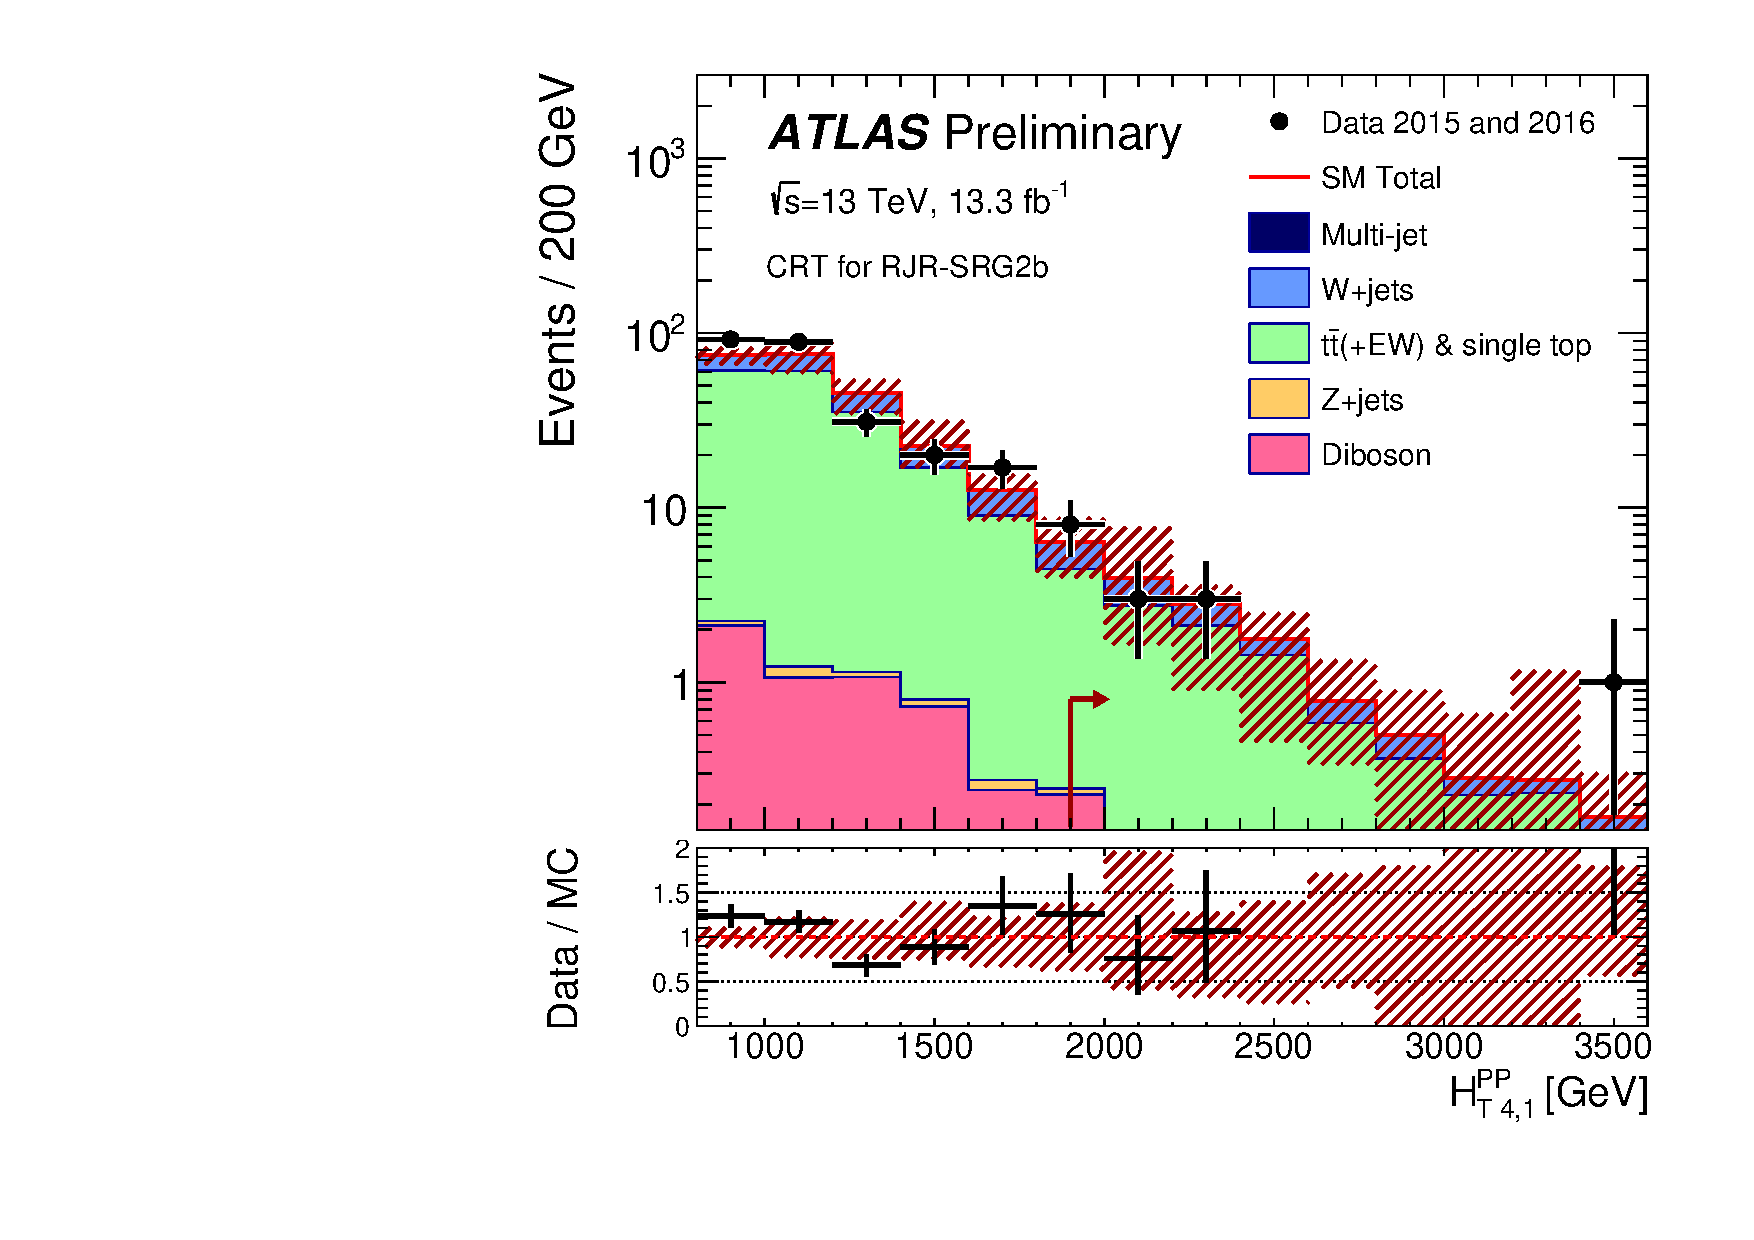
\includegraphics[width=0.45\textwidth]{figures/ATLAS-CONF-2016-078_INT/N-1Plots/AtlasStyle/Preliminary/CRT_SRJigsawSRG2b_LastCut_CRT_minusone}
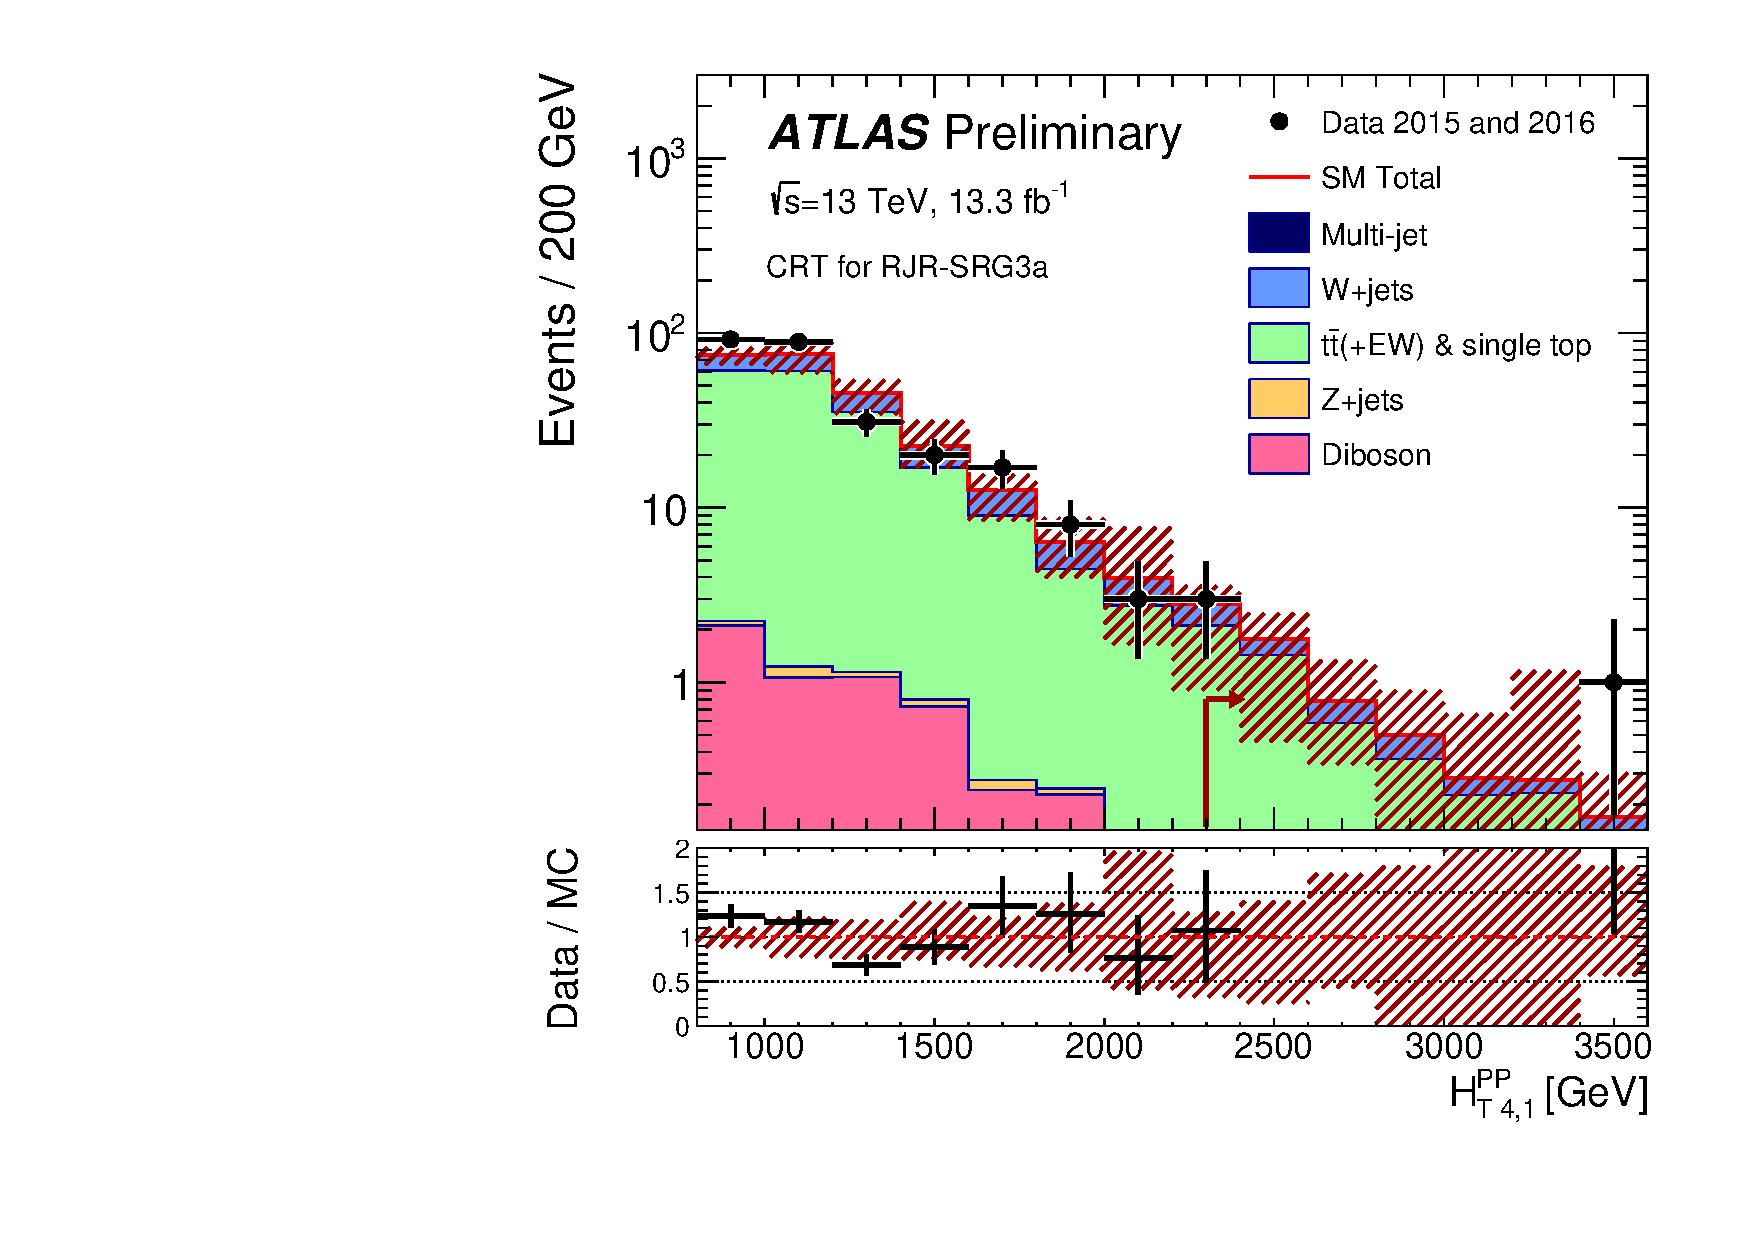
\includegraphics[width=0.45\textwidth]{figures/ATLAS-CONF-2016-078_INT/N-1Plots/AtlasStyle/Preliminary/CRT_SRJigsawSRG3a_LastCut_CRT_minusone}
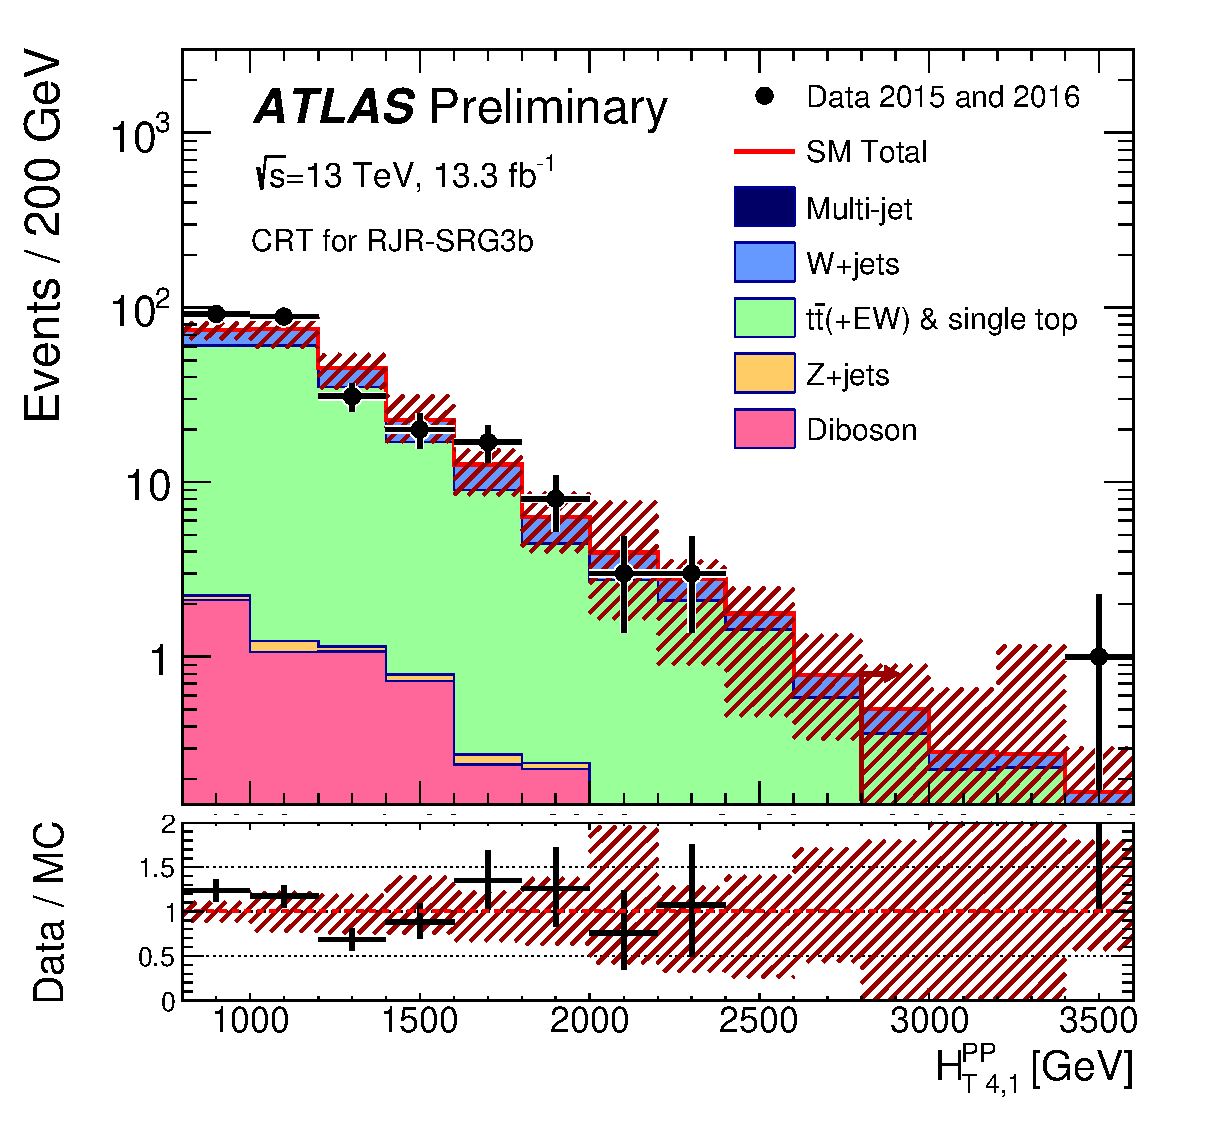
\includegraphics[width=0.45\textwidth]{figures/ATLAS-CONF-2016-078_INT/N-1Plots/AtlasStyle/Preliminary/CRT_SRJigsawSRG3b_LastCut_CRT_minusone}
\end{center}
\caption{Scale variable distributions for the gluino CRT regions.}
\label{fig:CRT_SRJigsawSRG1a_LastCut_CRT_minusone}
\end{figure}

\begin{figure}[tbph]
\begin{center}
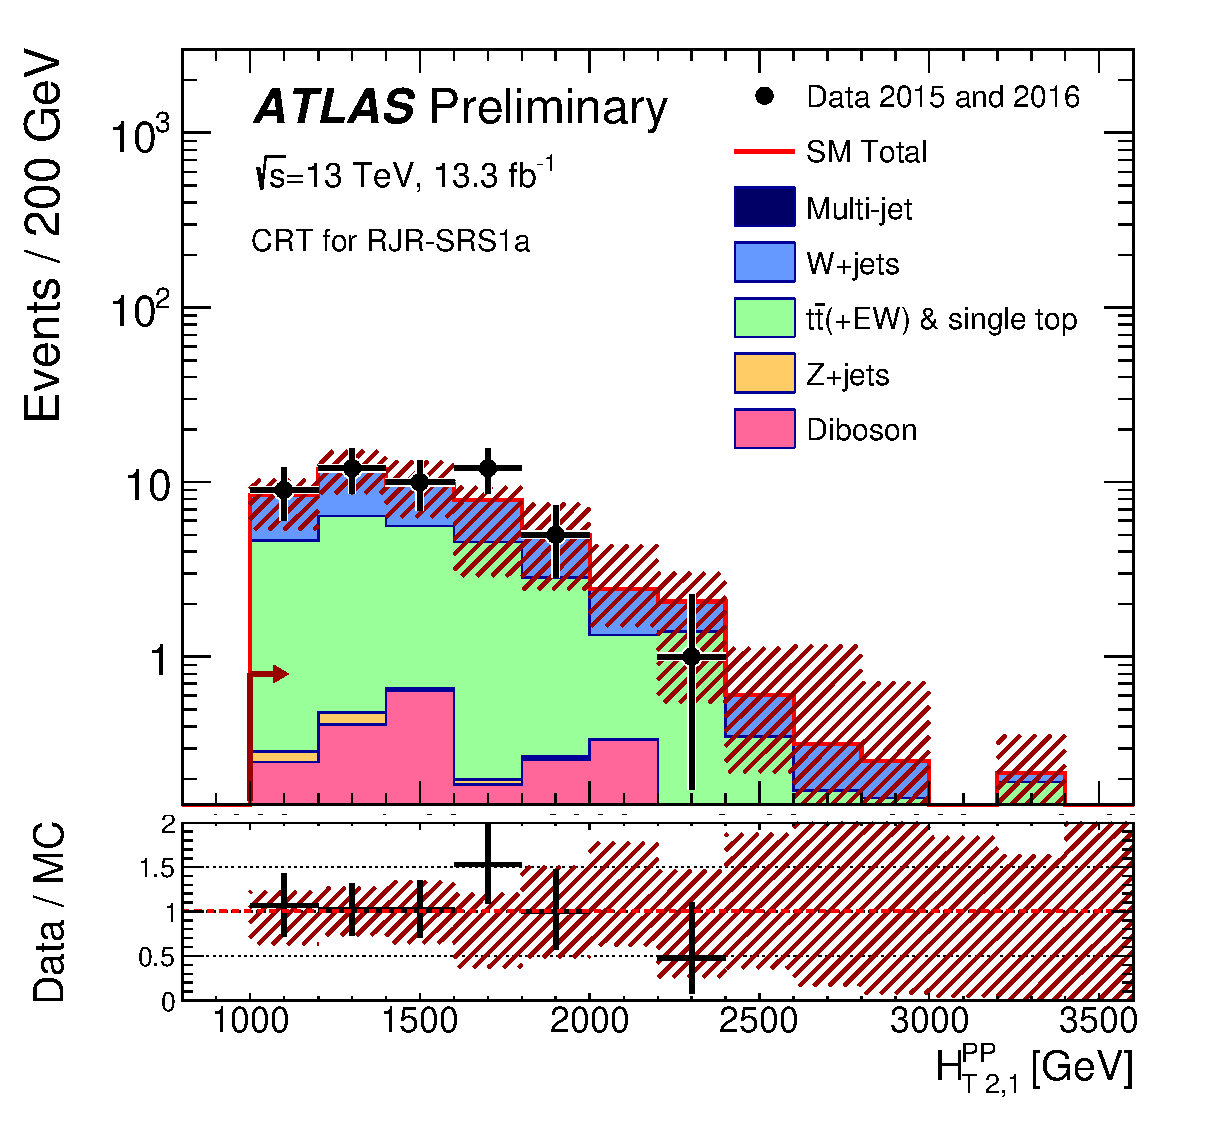
\includegraphics[width=0.45\textwidth]{figures/ATLAS-CONF-2016-078_INT/N-1Plots/AtlasStyle/Preliminary/CRT_SRJigsawSRS1a_LastCut_CRT_minusone}
\includegraphics[width=0.45\textwidth]{figures/ATLAS-CONF-2016-078_INT/N-1Plots/AtlasStyle/Preliminary/CRT_SRJigsawSRS1b_LastCut_CRT_minusone}
\includegraphics[width=0.45\textwidth]{figures/ATLAS-CONF-2016-078_INT/N-1Plots/AtlasStyle/Preliminary/CRT_SRJigsawSRS2a_LastCut_CRT_minusone}
\includegraphics[width=0.45\textwidth]{figures/ATLAS-CONF-2016-078_INT/N-1Plots/AtlasStyle/Preliminary/CRT_SRJigsawSRS2b_LastCut_CRT_minusone}
\includegraphics[width=0.45\textwidth]{figures/ATLAS-CONF-2016-078_INT/N-1Plots/AtlasStyle/Preliminary/CRT_SRJigsawSRS3a_LastCut_CRT_minusone}
\includegraphics[width=0.45\textwidth]{figures/ATLAS-CONF-2016-078_INT/N-1Plots/AtlasStyle/Preliminary/CRT_SRJigsawSRS3b_LastCut_CRT_minusone}
\end{center}
\caption{Scale variable distributions for the squark CRT regions.}
\label{fig:CRT_SRJigsawSRS1a_LastCut_CRT_minusone}
\end{figure}

\clearpage

\begin{figure}[tbph]
\begin{center}
\includegraphics[width=0.45\textwidth]{figures/ATLAS-CONF-2016-078_INT/N-1Plots/AtlasStyle/Preliminary/CRQ_SRJigsawSRC1_LastCut_CRQ_minusone}
\includegraphics[width=0.45\textwidth]{figures/ATLAS-CONF-2016-078_INT/N-1Plots/AtlasStyle/Preliminary/CRQ_SRJigsawSRC2_LastCut_CRQ_minusone}
\includegraphics[width=0.45\textwidth]{figures/ATLAS-CONF-2016-078_INT/N-1Plots/AtlasStyle/Preliminary/CRQ_SRJigsawSRC3_LastCut_CRQ_minusone}
\includegraphics[width=0.45\textwidth]{figures/ATLAS-CONF-2016-078_INT/N-1Plots/AtlasStyle/Preliminary/CRQ_SRJigsawSRC4_LastCut_CRQ_minusone}
\includegraphics[width=0.45\textwidth]{figures/ATLAS-CONF-2016-078_INT/N-1Plots/AtlasStyle/Preliminary/CRQ_SRJigsawSRC5_LastCut_CRQ_minusone}
\end{center}
\caption{Scale variable distributions for the compressed CRQ regions.}
\label{fig:CRQ_SRJigsawSRC1_LastCut_CRQ_minusone}
\end{figure}

\begin{figure}[tbph]
\begin{center}
\includegraphics[width=0.45\textwidth]{figures/ATLAS-CONF-2016-078_INT/N-1Plots/AtlasStyle/Preliminary/CRQ_SRJigsawSRG1a_LastCut_CRQ_minusone}
\includegraphics[width=0.45\textwidth]{figures/ATLAS-CONF-2016-078_INT/N-1Plots/AtlasStyle/Preliminary/CRQ_SRJigsawSRG1b_LastCut_CRQ_minusone}
\includegraphics[width=0.45\textwidth]{figures/ATLAS-CONF-2016-078_INT/N-1Plots/AtlasStyle/Preliminary/CRQ_SRJigsawSRG2a_LastCut_CRQ_minusone}
\includegraphics[width=0.45\textwidth]{figures/ATLAS-CONF-2016-078_INT/N-1Plots/AtlasStyle/Preliminary/CRQ_SRJigsawSRG2b_LastCut_CRQ_minusone}
\includegraphics[width=0.45\textwidth]{figures/ATLAS-CONF-2016-078_INT/N-1Plots/AtlasStyle/Preliminary/CRQ_SRJigsawSRG3a_LastCut_CRQ_minusone}
\includegraphics[width=0.45\textwidth]{figures/ATLAS-CONF-2016-078_INT/N-1Plots/AtlasStyle/Preliminary/CRQ_SRJigsawSRG3b_LastCut_CRQ_minusone}
\end{center}
\caption{Scale variable distributions for the gluino CRQ regions.}
\label{fig:CRQ_SRJigsawSRG1a_LastCut_CRQ_minusone}
\end{figure}

\begin{figure}[tbph]
\begin{center}
\includegraphics[width=0.45\textwidth]{figures/ATLAS-CONF-2016-078_INT/N-1Plots/AtlasStyle/Preliminary/CRQ_SRJigsawSRS1a_LastCut_CRQ_minusone}
\includegraphics[width=0.45\textwidth]{figures/ATLAS-CONF-2016-078_INT/N-1Plots/AtlasStyle/Preliminary/CRQ_SRJigsawSRS1b_LastCut_CRQ_minusone}
\includegraphics[width=0.45\textwidth]{figures/ATLAS-CONF-2016-078_INT/N-1Plots/AtlasStyle/Preliminary/CRQ_SRJigsawSRS2a_LastCut_CRQ_minusone}
\includegraphics[width=0.45\textwidth]{figures/ATLAS-CONF-2016-078_INT/N-1Plots/AtlasStyle/Preliminary/CRQ_SRJigsawSRS2b_LastCut_CRQ_minusone}
\includegraphics[width=0.45\textwidth]{figures/ATLAS-CONF-2016-078_INT/N-1Plots/AtlasStyle/Preliminary/CRQ_SRJigsawSRS3a_LastCut_CRQ_minusone}
\includegraphics[width=0.45\textwidth]{figures/ATLAS-CONF-2016-078_INT/N-1Plots/AtlasStyle/Preliminary/CRQ_SRJigsawSRS3b_LastCut_CRQ_minusone}
\end{center}
\caption{Scale variable distributions for the squark CRQ regions.}
\label{fig:CRQ_SRJigsawSRS1a_LastCut_CRQ_minusone}
\end{figure}


\subsection{Validation Regions}

As discussed in general terms above, we define a set of validations regions.
They validate the modeling of the backgrounds as we move closer to the SRs.
We define at least one validation region for each major background.

For the most important background \Zvv, we use a series of validation regions.
The primary validation region, which we label as VRZ, is defined by selecting lepton pairs of opposite sign and identical flavor which lie with 25 \GeV of the Z boson mass.
This selection has high purity for \Zll events as seen in simulation.
We treat the two leptons as contributions to the \met (as we did with the photon in CR$\gamma$).
This selection uses the same kinematic cuts as the signal region.
We also define two VRs using the same event selection but looser kinematic cuts, which we label VRZa and VRZb.
VRZa has a loosened selection on \HFnm{PP}{1}{1}.
VRZb is looser in the primary scaleful variable  (\HTFnm{PP}{2}{1} or \HTFnm{PP}{4}{1}).
These two validation regions allow us to test the modeling of each of these variables individually.

For the compressed regions, these $Z$ validation region were found lacking.
The leptons are highly boosted in the compressed case, and the lepton acceptance was quite low due to lepton isolation requirements in \deltaR.
Instead, two fully hadronic validation region were developed for the compressed regions.
The first, VRZc has identical requirements to the signal regions except we require \dphiISR to be \textit{smaller} than the value of the corresponding signal region.
From simulation, this region with at least 50\% pure in $Z$ events, which was considered enough to validate the $Z$ modeling considering the extreme portion of phase space considered.
For additional validation region statistics, we also developed VRZca, which again uses the loosest set of cuts from each signal region.
Note this means that each compressed signal region has an identical VRZca.

The top and $W$ validation regions use the same event selection as the corresponding control regions with stronger cuts on the scaleful variables.
For example, in SRS3a, VRT has the following kinematic selection, with a $b$-tag required:
\begin{table}[H]
\label{tab:vrw_kinematic_selection}
\begin{tabular}{|l|l|}
\hline
Variable & VRT cut \\ \hline
$H_{\textrm 1,1}^{\textrm ~PP}/H_{\textrm 2,1}^{\textrm ~PP} \geq$ & 0.5 \\ \hline
$H_{\textrm 1,1}^{\textrm ~PP}/H_{\textrm 2,1}^{\textrm ~PP} \leq$ & 0.98 \\ \hline
$p_{\textrm PP,~z}^{\textrm ~lab} / \left( p_{\textrm PP,~z}^{\textrm ~lab}+H_{\textrm T~2,1}^{\textrm ~PP}\right) \leq $ & 0.6 \\ \hline
$p_{\textrm j2,~T}^{\textrm ~PP}/H_{\textrm T~2,1}^{\textrm ~PP} \geq $ & 0.13 \\ \hline
$\Delta_{\textrm  QCD} > $ & 0.001 \\ \hline
$H_{\textrm T~2,1}^{\textrm ~PP}>$ & 1800 \GeV \\ \hline
$H_{\textrm 1,1}^{\textrm ~PP} >$ & 1600 \GeV \\ \hline
\hline
\end{tabular}
\end{table}
The cuts on the scaleless cuts shown are identical to those in \Cref{tab:crw_kinematic_selection}, but the selections on scaleful cuts $H_{\textrm T~2,1}^{\textrm ~PP}$ and $H_{\textrm 1,1}^{\textrm ~PP}$ are restored to those of the signal region, as shown in \Cref{tab:squark_srs}.
Thus, these regions have a kinematic selection between the corresponding CRT and the signal region selection.
To provide additional validation, we also define auxiliary VRs which loosen the cuts on the scale variables.
VRTa (VRWa) as VRT (VRW) loosens the selection on \HFnm{PP}{1}{1} to that off the control region, while still requiring the cut on the primary scale variable.
The opposite logic is required for VRTb and VRWb: the primary scale variable cut is loosened, while still requiring the \HFnm{PP}{1}{1} selection of the signal region.

The final set of validation regions are those defined to check the QCD background.
VRQ is defined to be identical to the corresponding CRQ, but again we use the full SR region cuts for the scaleful variables.
This selection is then closer to the corresponding signal region to validate the CRQ estimate.
We also define the auxiliary validation regions VRQa and VRQb for the noncompressed signal regions.
In this case, we reimpose one of the two inverted cuts in CRQ with respect to the signal regions, to make each one even closer to the SRs.
In CRQa (CRQb), we reimpose the \HFnm{PP}{1}{1} ($\Delta_{\mathrm{QCD}}$).

For the compressed case, we again define a separate validation region, due to the special kinematics probed.
We construct a validation region which is the same as CRQ, with $.5 < \risr < R_{\text{ISR, SR}}$, where $R_{\text{ISR, SR}}$ is the cut on \risr~ in the corresponding SR.
Again, this can be seen as probing ``in between'' the CR and SR in phase space.

The results of this validation can be seen in \Cref{fig:vr_summary}.
Each bin is \textit{pull} of the validation region corresponding to a particular signal region.
This is defined
\begin{align}
\text{Pull} = \frac{N_{\mathrm{obs}} - N_{\mathrm{pred}}}{\sigma_{\mathrm{tot}}}
\end{align}
where $\sigma_{\mathrm{tot}}$ is the total uncertainty folding in all systematic uncertainties.

In the case that the backgrounds are properly estimated in the validation regions, the pulls will form a Gaussian distribution with a mean of 0 and standard deviation of 1.
In our case, we see that most pulls are negative, with fewer positive pulls.
This indicates we have conservatively measured the Standard Model backgrounds.

\begin{figure}[tbp]
\caption{Summary of the validation region pulls.
Dashes indicate the validation region is not applicable to the given signal region.} \label{fig:vr_summary}
\includegraphics[width=.9\linewidth]{ATLAS-CONF-2016-078/fig_05b}
\end{figure}

%\subsection{R Z/$\gamma$ method}
\subsection{Systematic Uncertainties}

In this section we discuss the uncertainties.
These generally fall into four categories: theoretical generator uncertainties, uncertainties on the CR to SR extrapolations, uncertainties on the data-driven transfer factor corrections, and object reconstruction uncertainties.
We discuss each of these categories here.
A summary of the uncertainties is available in \Cref{tab:systematics-table}.
MC statistics
\begin{table}[tbp]
\scriptsize
\begin{center}
\begin{tabular}{| l | l |}
\hline
Systematic                        & Uncertainty Description                                                   \\
\hline\hline
MC statistics                     & Simulation statistics in the signal region                                \\ \hline
Theory Z                          & Theoretical  on $Z$ cross-section                                         \\ \hline
Theory W                          & Theoretical  on $W$ cross-section                                         \\ \hline
Theory Top                        & Theoretical  on $t$ cross-section, radiation tune, and fragmentation tune \\ \hline
Theory Diboson                    & Flat theoretical on diboson cross-section                                 \\ \hline
$\Delta\mu_{Z,\mathrm{+jets}}$    & CRY extrapolation to SR                                                   \\ \hline
$\Delta\mu_{W,\mathrm{+jets}}$    & CRW extrapolation to SR                                                   \\ \hline
$\Delta\mu_{\mathrm{ Top}}$       & CRT extrapolation to SR                                                   \\ \hline
$\Delta\mu_{\mathrm{ Multijet}}m$ & CRQ extrapolation to SR                                                   \\ \hline
%gamma\_stat\_SR\_cuts\_bin\_0    & CRY statistical                                                           \\ \hline
CR$\gamma$ corr. factor $\kappa$  & $\kappa$ factor                                                           \\ \hline
Multijet method                   & Jet smearing uncertainty                                                  \\ \hline
Jet/MET                           & Jet/MET uncertainties                                                     \\ \hline
% alpha\_JET\_GroupedNP\_1      & JES NP group 1 \\ \hline
% alpha\_JET\_GroupedNP\_2      & JES NP group 2            \\ \hline
% alpha\_JET\_GroupedNP\_3      & JES NP group 3            \\ \hline
% alpha\_JER                  & JER             \\ \hline
% alpha\_MET\_SoftTrk\_ResoPerp & Soft \met resolution perpendicular to hard object system          \\ \hline
% alpha\_MET\_SoftTrk\_ResoPara & Soft \met resolution parellel to hard object system           \\ \hline
% alpha\_MET\_SoftTrk\_Scale    & Soft \met scale            \\ \hline
\end{tabular}
\caption{Description of the systematic uncertainties in the analysis. }
\label{tab:systematics-table}
\end{center}
\end{table}




%%% Local Variables:
%%% mode: latex
%%% TeX-master: t
%%% End:


The theoretical generator uncertainties are evaluated by using alternative simulation samples.
In the case of the \zjets~ and \wjets~ backgrounds, the related theoretical uncertainties are estimated by varying the renormalization, factorization, and resummation scales by two, and decreasing the nominal CKKW matching scale by 5 \GeV and 10 \GeV respectively.
In the case of \ttbar production, we compare the nominal \textsc{Powheg-Box} generator with MG5\_aMC@NLO, as well as comparing different radiation and generator tunes.
As stated above, we account for the uncertainty on the small diboson background by imposition of a flat 50\% uncertainty.

The uncertainties on the normalization factors $\mu_{\text{background}}$ are listed in \Cref{tab:systematics-table} as $\Delta\mu_{\text{background}}$.
%There is one normalization factor $\mu$ for each major background, and their uncertainties, especially $\mu_Z$, are often dominant for the measurement in many signal regions.
In previous analyses, these uncertainties have often been dominant, especially $\Delta\mu_{Z,\mathrm{+jets}}$, as these uncertainties represent our misunderstanding of the total event yields of the Standard Model backgrounds in the signal regions.
The statistical uncertainty from the control region is generally the most important component of these uncertainties.

There are two uncertainties from the data-driven corrections to the transfer factors.
The first is the uncertainty on $\kappa$, which we derived by varying the \met requirements of the auxiliary CRZVL and CR$\gamma$VL control regions.
The other is the uncertainty is that assigned to the jet smearing method, which is derived using the method in~\cite{SUSY-2011-20}.

The final set of uncertainties are those related to object reconstruction.
In the case of a hadronic, the important uncertainties are those assigned to the jet energy and \met.
The uncertainties on the lepton reconstruction and $b$-tagging uncertainties were found to be negligible in all SRs.
The measurement of the jet energy scale (JES) uncertainty is quite complicated, and described in ~\cite{Aad:2011he,Aad:2012vm,ATL-PHYS-PUB-2015-015}.
After a complicated procedure to decorrelate the various components of the JES uncertainty, there are three remaining components.
The jet energy resolution uncertainty is estimated using the methods discussed in Refs.~\cite{Aad:2012ag,ATL-PHYS-PUB-2015-015}.
These uncertainties are included in the the total Jet/MET uncertainty.

The \met soft term uncertainties are described in ~\cite{PERF-2014-04,ATL-PHYS-PUB-2015-023,ATL-PHYS-PUB-2015-027}.
The uncertainty on the \met soft term resolution is parameterized into a component parallel to direction of the rest of the event (the sum of the hard objects \pt) and a component perpendicular to this direction.
We also derive an uncertainty on the \met soft term scale.
These uncertainties are also included in the total Jet/MET uncertainty.
The uncertaint
There is also an uncertainty on the \met soft term scale.

\section{Background-only fit, model-independent fit, and model-dependent fit}

The maximum likelihood fit described above can be used with a variety of event count inputs.
We use three separate fit classes, which we call \textit{background-only}, \textit{model-independent}, and \textit{model-dependent} fits.
In terms of the likelihood function inputs, these can be seen as including a different list of event counts $\bm{b}$

The background-only fit estimates the background yields in each signal region.
This fit use only the control region event yields as inputs; they do not include the information from the signal regions besides the simulation event yield.
The cross-contamination between CRs is also fit by this procedure.
The output of the background-only fit is the set of \textit{fitted} simulated event counts in the signal and validation regions,

In the case no excess is observed, we use a model-independent fit to set upper limits on the possible number of possible beyond the Standard Model events in each SR.
These limits are derived using the same procedure as the background-only fit, with two additional pieces of information included in the fitting procedure.
We include the SR event count as an additional input and fit an additional normalization parameter $\mu_{\text{signal}}$, which we call the signal strength.
We use the $CL_{\mathrm{S}}$ procedure~\cite{Feldman:1997qc}, to derive the the observed and expected limits on the number of events from BSM phenomena in each signal region.

Model-dependent fits are used to set exclusion limits on the specific SUSY models in the sparticle-LSP grids.
It is identical to the background-only fit but including the signal model simulation event yield and the additional $\mu_{\text{signal}}$ normalization parameter.
As noted when we introduced \Cref{fig:sr_schematic}, the exclusion contours from previous model-dependent fits motivate the signal region design.
If no excess is found, we set limits on each of the simplified signal models with various mass splittings.
